\section{Datasets and simulated events} \label{datasets_and_MC_samples}

\subsection{Data samples}

The data sample used in this analysis consists of a CMS data sample recorded at 2016, at $sqrt{s} = $ 13 \TeV, with 25 $ns$ bunch separation. This data sample is composed only by events that were certified from all CMS subsystems and reconstruction specialists as good for physics analysis.

This data sample corresponds to 35.86 $fb^{-1}$ of integrated luminosity~\cite{CMS-PAS-LUM-17-001}.

\subsection{Simulated datasets}
\label{sec:datasets}

Simulation of events at CMS is done via Monte Carlo methods (from here on, simply called MC). Pseudo-random events are generated within the physics of the related processes in which we are interested starting from  hard-scattering processes, at parton (constituents of the proton)  level, usually  with matrix element generators. These handle the incoming and outcoming partons so that they follow some pre-defined theoretical model. The matrix element generator, working on the parton level, allow us to extract the momentum distribution of the parton as a function of the $q^2$ (transferred momentum) of the collision.  MC generators use the so-called parton distribution functions (PDFs) to sample values of momenta and can account for different order of perturbations, like NLO (next-to-leading order), NNLO (next-to-next-to-leading order), and so on.

After the hard-scattering, the \textbf{showering} process simulates the radiation emission by gluons and quarks in the initial and final states. Along the hard interaction, the other proton constituents may also interact through soft interaction. This part of the simulation is called \textbf{multiple parton interaction} (MPI). The last component of the simulation is the \textbf{hadronization},  in which quarks and gluons compose to form hadrons. These can decay according to specific models, as predicted in the case of heavy hadrons, like B hadrons and taus etc. This imposes the QCD confinement to low energy quarks and gluons~\footnote{QCD forbids coloured objects to exist in non-asymptotic states. They must decays to more complex systems, until they form stable colorless states.}.

Usually, different generators are used to simulate a process. Each specialized in one or more steps.

A summary of the signal and background MC samples used is presented in Table~\ref{tab:MC}. These simulated data are comparable with the proton-proton collision using 2016 data conditions and the \textbf{pileup}~\footnote{Each LHC collision recorded by CMS, is composed not by a single $pp$ interaction, but by bunches of protons crossing each other. In this case, a hard interaction is actually surrounded by many soft interaction between adjacent protons. The extra activity produced in these interactions, and caught by the detector, is called \textbf{pileup} and has its signal mixed with the hard one. Since, during the data taking, the number of pileup interactions varies according to the instantaneous luminosity, the MC are mixed some soft interaction only sample, called Minimum Bias. The number of mixed soft interaction (pileup events) is governed by a Poisson distribution with a pre-defined mean. The MC samples are then reweighted to match the same distribution of primary vertexes for the corresponding Data. Systematics related to this procedure will be discussed later. A pioneer work on this subject, at CMS, is the master dissertation from Eliza Melo~\cite{tese_eliza} - Rio de Janeiro University.} events are added to the simulated event in this step. The pileup events distribution used is modeled as a Poisson pdf (probability distribution function) with mean of 23 events, as recommended by CMS. Detector response in the MC samples is simulated using a detailed description of the CMS detector, based on \GEANTfour~\cite{Agostinelli:2002hh}.

The signal MC samples are simulated for the Higgs bosons decaying to $\Upsilon(nS) (\rightarrow \mu\mu) + \gamma$  channels with POWHEG v2.0~\cite{powheg2_1,powheg2_2,powheg2_3}, at next-to-leading order (NLO) of Feynman graphs computation, for the following production modes: gluon-gluon fusion (ggF), vector boson fusion (VBF), associated production (VH) and associated top production (ttH), with cross-section summarized at table \ref{tab:MC}. An extensive review of these production modes can be found at~\cite{DJOUADI20081}. The \PYTHIA 8 generator~\cite{SJOSTRAND2008852,Sjostrand:2014zea} is used for hadronization and fragmentation with underlying event tune CUETP8M1~\cite{Khachatryan:2015pea}. The parton distribution functions (pdf) NNPDF3.0~\cite{NNPDF3} are used. 

 For Z decaying to $\Upsilon(nS) (\rightarrow \mu\mu) + \gamma$  channels, the signal samples are simulated with \MADGRAPH5 $\_$\MCATNLO 2.6.0 matrix element generator~\cite{Alwall2014} at next leading order and the \PYTHIA 8 generator~\cite{SJOSTRAND2008852,Sjostrand:2014zea} for hadronization and fragmentation with underlying event tune CUETP8M1~\cite{Khachatryan:2015pea}.

The Drell-Yan process, $pp \rightarrow \Z \rightarrow \mu\mu \gamma_{FSR}$, results in the same final state as the signal. This process exhibits a peak in the three-body invariant mass, $m_{\mu\mu\gamma}$, at the \Z boson mass, $m_{Z}$, and it is a resonant background for this channel, therefore referred to as Peaking or Resonant Background. 

It is taken into account when deriving the upper limit on the branching fraction for Z$\rightarrow \Upsilon(nS) + \gamma \rightarrow \mu\mu + \gamma$. The \MADGRAPH5 $\_$\MCATNLO 2.6.0 matrix element generator~\cite{Alwall2014} at leading order, interfaced with \PYTHIA 8.226 for parton showering and hadronization with tune CUETP8M1~\cite{Khachatryan:2015pea}, is used to generate a sample of these resonant background events. The photons in these events are all produced as final-state radiation from the $ Z \rightarrow \mu\mu$ decay and therefore the $m_{\mu\mu\gamma}$ distribution peaks at the \Z boson mass and there is no continuum contribution.  

Similarly, the Higgs boson Dalitz decay~\cite{PhysRevD.55.5647}, $H \rightarrow \gamma^{*} \gamma\rightarrow \mu\mu + \gamma$, is a Resonant Background (resonant) to $H \rightarrow \Upsilon(nS) \rightarrow \mu\mu + \gamma$. It is simulated at NLO with \MADGRAPH5 $\_$\MCATNLO 2.6.0 matrix element generator~\cite{Alwall2014} at next-to-leading order and the \PYTHIA 8 generator~\cite{SJOSTRAND2008852,Sjostrand:2014zea} for hadronization and fragmentation with underlying event tune CUETP8M1~\cite{Khachatryan:2015pea}. This Higgs Dalitz Decay sample, was generated only for the ggF production mode, but its cross-section was rescaled to the full Higgs cross-section. This process will present a small contribuition of selected events, so this approximation should be sufficient for the Higgs Resonant Background modeling.

There are also background processes that do not give resonance peaks in the three-body invariant mass spectrum. They are modeled from data, as it will be explained latter in more details.
 
\begin{table}[htp]
\begin{center}
\caption{Datasets simulated (MC) for 2016 conditions. Assuming that $\sigma (pp\rightarrow$ H), taking into consideration all the simulated Higgs production modes, is 55.13 $pb$~\cite{CERNYellowReportPageAt13TeV} and  $\sigma (pp\rightarrow Z \rightarrow \mu\mu$ ) is 57094.5 $pb$, including the next-to-next-to-leading order
(NNLO) QCD contributions, and the next-to-leading order (NLO) electroweak corrections from FEWZ (Fully Exclusive W and Z Production) 3.1~\cite{FEWZ} calculated using the NLO PDF set NNPDF3.0, with the phase space selection in invariant mass of the dimuon system of $m_{\mu\mu} > 50$ GeV. For the Higgs Dalitz $\sigma$, we consider only the gluon fusion contribution ($\sigma_{\text{ggF}}  = $ 48.6 $pb$)~\cite{CERNYellowReportPageAt13TeV}. The Higgs Dalitz Decay $BR_{SM}$ and the $Z \rightarrow \mu\mu\gamma_{FSR}$ were obtained with MCFM 6.6~\cite{CAMPBELL201010} (as in the CMS search for Higgs Dalitz Decay in at $\sqrt{s} =$ 8 TeV~\cite{dalitz_decay_8_Tev}) and with \MADGRAPH5 $\_$\MCATNLO, respectively. The $BR^{PDG}_{\Upsilon(1S,2S,3S) \rightarrow \mu\mu} = \text{(2.48, 1.93, 2.18)} \times 10^{-2}$ is quoted from Particle Data Group report (PDG)~\cite{pdg_2020}. The "Effective $\sigma$" for the signal samples is $\sigma(pp \rightarrow Z(H)) \times BR_{SM} \times BR^{PDG}_{\Upsilon(nS) \rightarrow \mu\mu}$.}
%
%\begin{tabular}{lcccc} \hline
%Physics Processes &  $\sigma$ in pb   & Branching Ratio (BR$_{SM}$) & Generator & Sample Type \\ \hline
%H$\rightarrow  \Upsilon(1S) +\gamma$ & 7.1996$\times 10^{-9}$ &5.22$\times 10^{-9}$ & PYTHIA8 & Signal \\ 
%H$\rightarrow  \Upsilon(2S) +\gamma$ & 1.5242$\times 10^{-9}$ &1.42$\times 10^{-9}$  & PYTHIA8 & Signal \\ 
%H$\rightarrow  \Upsilon(3S) +\gamma$ & 1.1033$\times 10^{-9}$ &9.10$\times 10^{-10}$ & PYTHIA8 & Signal \\ \hline
%Z$\rightarrow  \Upsilon(1S) +\gamma$ & 6.7965$\times 10^{-5}$ &4.88$\times 10^{-8}$ & PYTHIA8 & Signal \\ 
%Z$\rightarrow  \Upsilon(2S) +\gamma$ & 2.6887$\times 10^{-5}$ &2.44$\times 10^{-8}$ &  PYTHIA8 & Signal \\
%Z$\rightarrow  \Upsilon(3S) +\gamma$ & 2.3400$\times 10^{-5}$ &1.88$\times 10^{-8}$ &  PYTHIA8 & Signal \\  \hline \hline
%H$\rightarrow \gamma\gamma^{*}$ Dalitz Decay & 1.8614$\times 10^{-3}$ & 3.83$\times 10^{-5}$ & --- & Peaking Background \\ 
%Z$\rightarrow  \mu\mu\gamma_{FSR}$ & 7.9260$\times 10^{-2}$& --- & --- & Peaking Background \\ \hline
%\end{tabular}





\begin{tabular}{lcccc} \hline
Physics Processes & Branching Ratio (BR$_{SM}$)  & Effective $\sigma$ (in pb) & Generator & Sample Type \\ \hline
H$\rightarrow  \Upsilon(1S) +\gamma$ &5.22$\times 10^{-9}$ & 7.14$\times 10^{-9}$ & \POWHEG 2.0 & Signal \\ 
H$\rightarrow  \Upsilon(2S) +\gamma$ &1.42$\times 10^{-9}$ &  1.51$\times 10^{-9}$ & \POWHEG 2.0 & Signal \\ 
H$\rightarrow  \Upsilon(3S) +\gamma$ &9.10$\times 10^{-10}$ & 1.10$\times 10^{-9}$ & \POWHEG 2.0 & Signal \\ \hline
Z$\rightarrow  \Upsilon(1S) +\gamma$ &4.88$\times 10^{-8}$ & 6.80$\times 10^{-5}$ & \MADGRAPH5  & Signal \\ 
Z$\rightarrow  \Upsilon(2S) +\gamma$ &2.44$\times 10^{-8}$ & 2.69$\times 10^{-5}$ &  \MADGRAPH5  & Signal \\
Z$\rightarrow  \Upsilon(3S) +\gamma$ &1.88$\times 10^{-8}$ & 2.34$\times 10^{-5}$ &  \MADGRAPH5  & Signal \\  \hline \hline
H Dalitz Decay & 3.83$\times 10^{-5}$ & 2.13$\times 10^{-3}$ &\MADGRAPH5 & Resonant Background \\ 
Z$\rightarrow  \mu\mu\gamma_{FSR}$ & --- & 7.93 $\times 10^{-2}$ & \MADGRAPH5  & Resonant Background \\ \hline
\end{tabular}
\label{tab:MC}
\end{center}
\end{table}

The number of simulated events is rescaled by the effective $\sigma$, from Table~\ref{tab:MC}, in order to match 35.86 $fb^{-1}$ of integrated luminosity, from the recorded data. Being $N = \sigma \mathcal{L}$, $N$ in the number of events for a process, $\sigma$ is the cross-section and $\mathcal{L}$ is the integrated luminosity, the reweighting factor, for a simulated sample is:

\begin{equation}
\label{eqn:mc_weight}
w_{MC} = \frac{\sigma \mathcal{L}}{N_{sim}},
\end{equation}
where $N_{sim}$ is the number of simulated events for a specific process.

The simulated sample are also corrected by the data pileup distribution, since the pileup distribution of MC is different from the pileup distribution of data. The way to correct the MC is to assign a weight to each bin of the MC pileup distribution, with repect to the data. The rescaling is defined as the ratio between normalized pileup (PU) distribution for Data and MC.

\begin{equation}
\label{eqn:mc_weight}
w_{PU}(n) = \frac{P^{Data}_{PU}(n)}{P^{Sim}_{PU}(n)},
\end{equation}
where $n$ is the number of interaction per bunch crossing (pileup).

\section{Contribution of the \texorpdfstring{$\Upsilon(nS)$} p polarisation}
\label{sec:polarization}

% Tem que ter esse erro de digitacao no titulo senao nao compila.
Measurements of quarkonium polarization observables may yield information about quarkonium production mechanisms that are not available from the study of unpolarized cross sections alone. The three polarization states of a $J = 1$ quarkonium can be specified in terms of a particular coordinate system in the rest frame of the quarkonium. This coordinate system is often called the "spin-quantization frame". 

In a hadron collider, $\Upsilon(1S,2S,3S)$ are reconstructed through their electroweak decays into a lepton pair. The information about the polarization of the quarkonium state is encoded in the angular distribution of the leptons. This angular distribution is usually described in the quarkonium rest frame with respect to a particular spin-quantization frame~\cite{Brambilla:2011bph}. The polarization of the  $\Upsilon(1S,2S,3S)$ is not simulated for signal MC sample and we only apply a reweighting scale factor to each event and so we can emulate the polarization effects~\cite{PhysRevD.83.031503}. Figure \ref{fig:ZUpsilonPolarization} present the distributions of $\cos \Theta$ of $\Upsilon \rightarrow \mu\mu$, 
% and $\gamma^{*} \rightarrow \mu\mu$, 
where $\Theta$ is the angle between the positive muon and the $\Upsilon$ in the Z (Higgs) rest-frame. At Table \ref{fig:polTable} we show the analytical functions used to describe the extremes scenarios (Unpolarized, Transverse Polarization and Longitudinal Polarization) reweighting, presented in this analysis. 

It is worth stating that, for the Higgs decay, only the Transverse Polarization is considered. For the Z decay, because of its spin nature, the Unpolarized scenario is used as the nominal one, and the effects of the two other extremes (Transverse Polarization and Longitudinal Polarization) are quoted as systematics.


% \begin{figure}[!htbp]
% \begin{center}
% 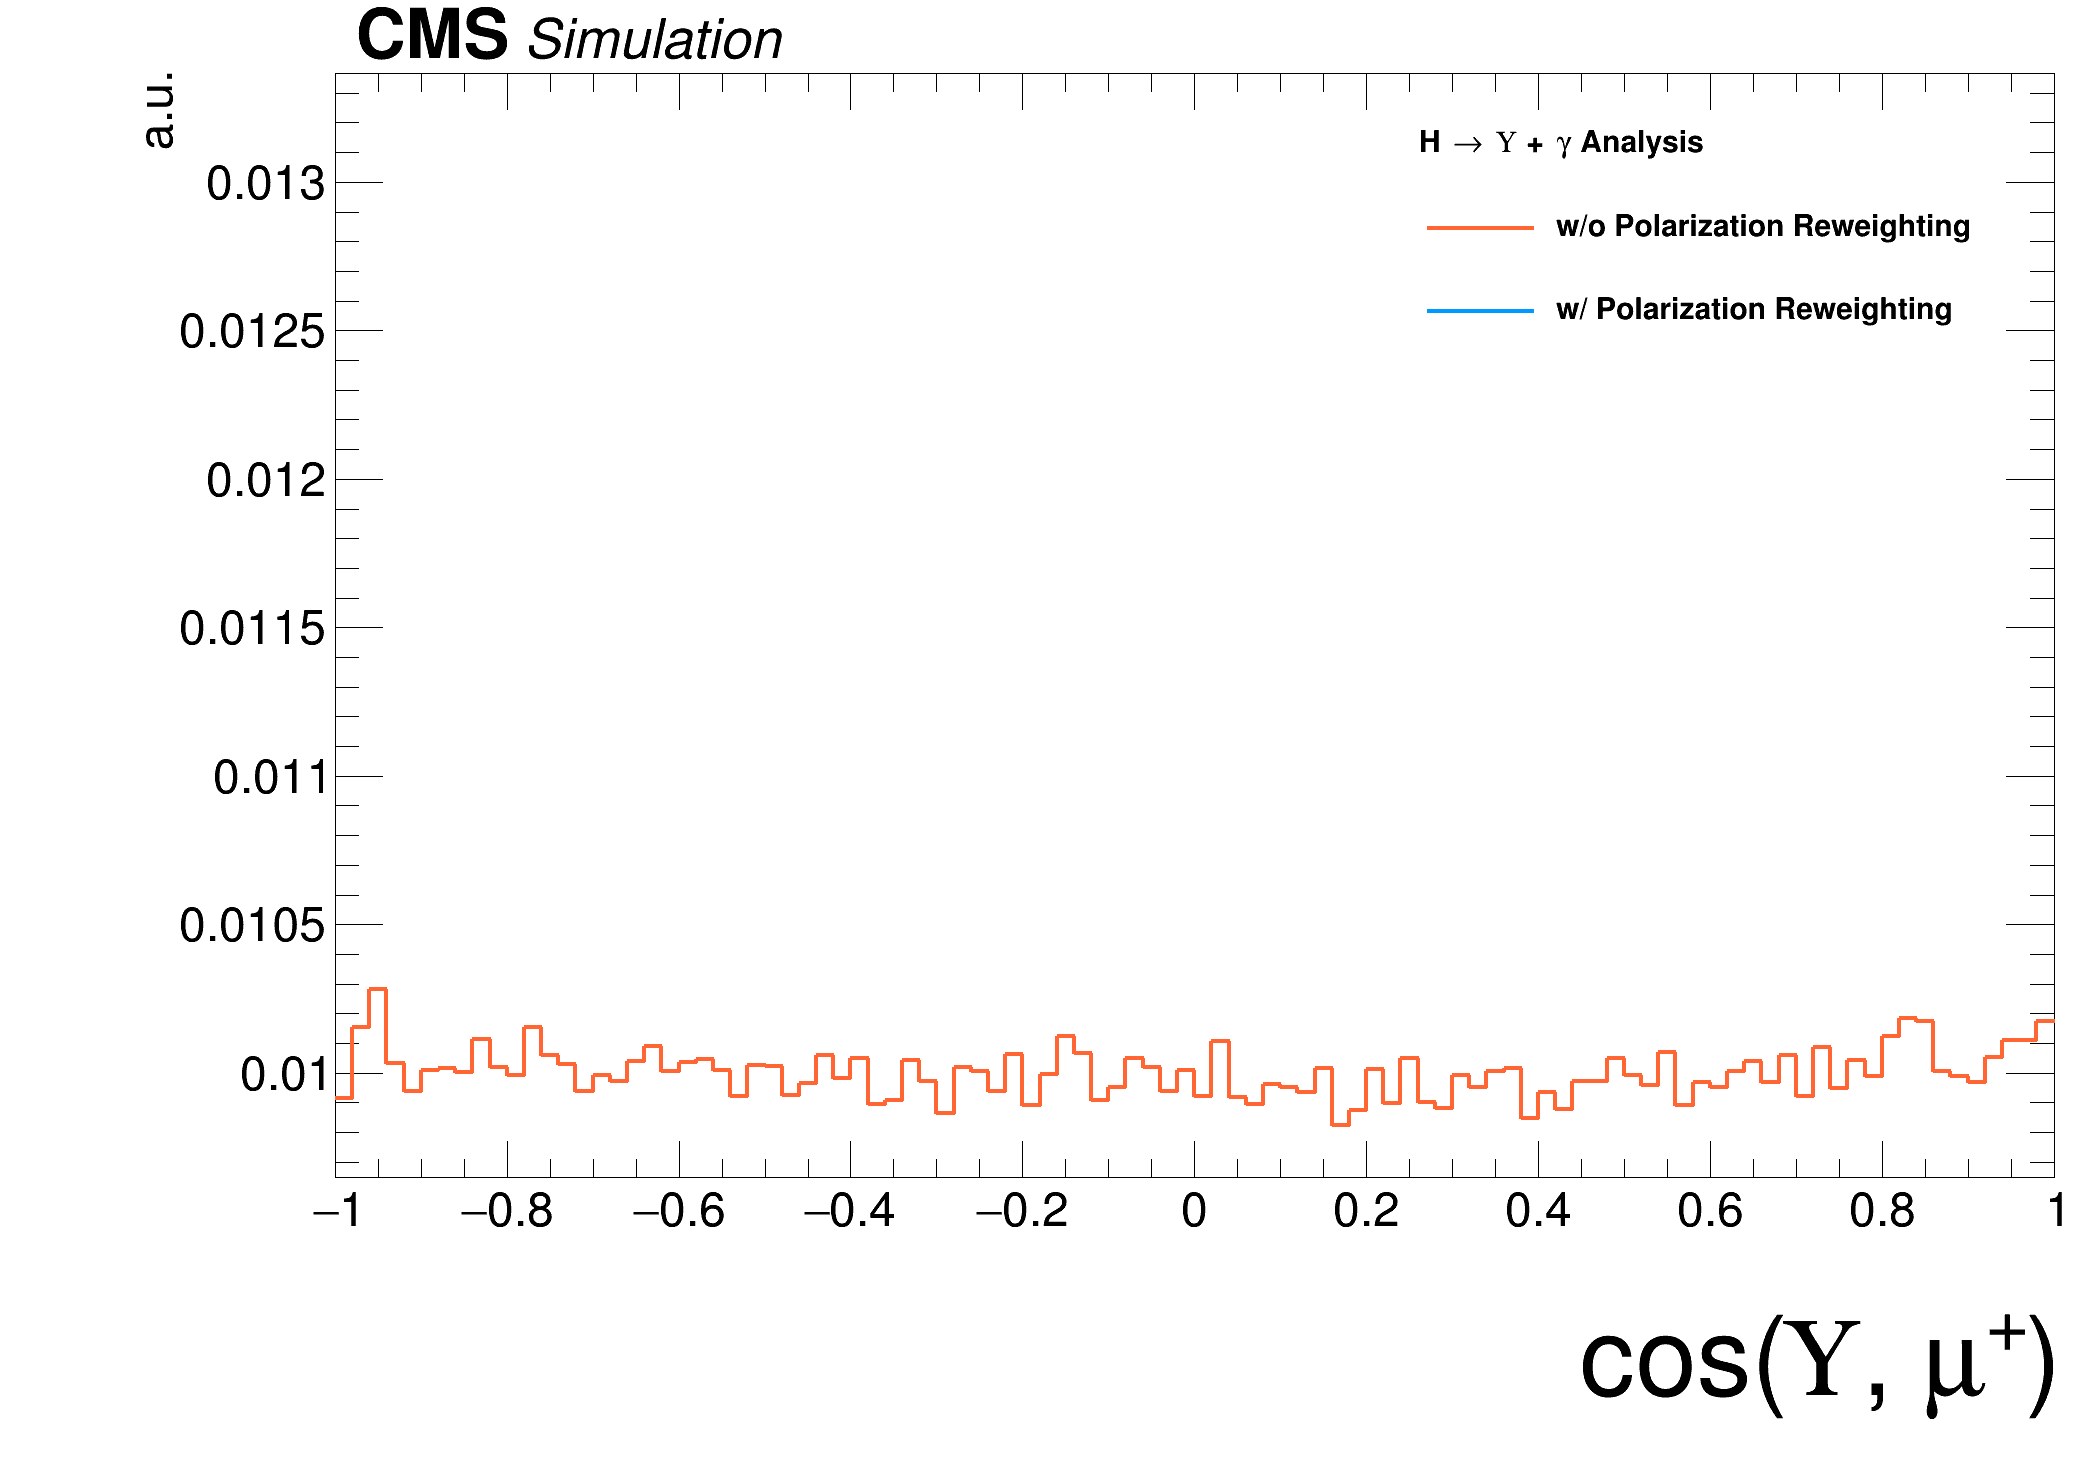
\includegraphics[width=0.50\textwidth]{figures_and_tables/outputPlots/HtoUpsilon_Cat0_ZZZZZ/mc/polarizatioReweight/h_Gen_COS_theta}
% \end{center}\vspace*{-.5cm}
% \caption{Distributions of $\cos \theta$ of $\Upsilon \rightarrow \mu\mu$ and $\gamma^{*} \rightarrow \mu\mu$ The orange distribution is the $H \rightarrow  \Upsilon(1S,2S,3S) + \gamma$ sample before reweighting; the blue distribution is $H \rightarrow  \Upsilon(1S,2S,3S)$ sample after reweighting.}
% \label{fig:HUpsilonPolarization}
% \end{figure}


\begin{figure}[!htbp]
\begin{center}
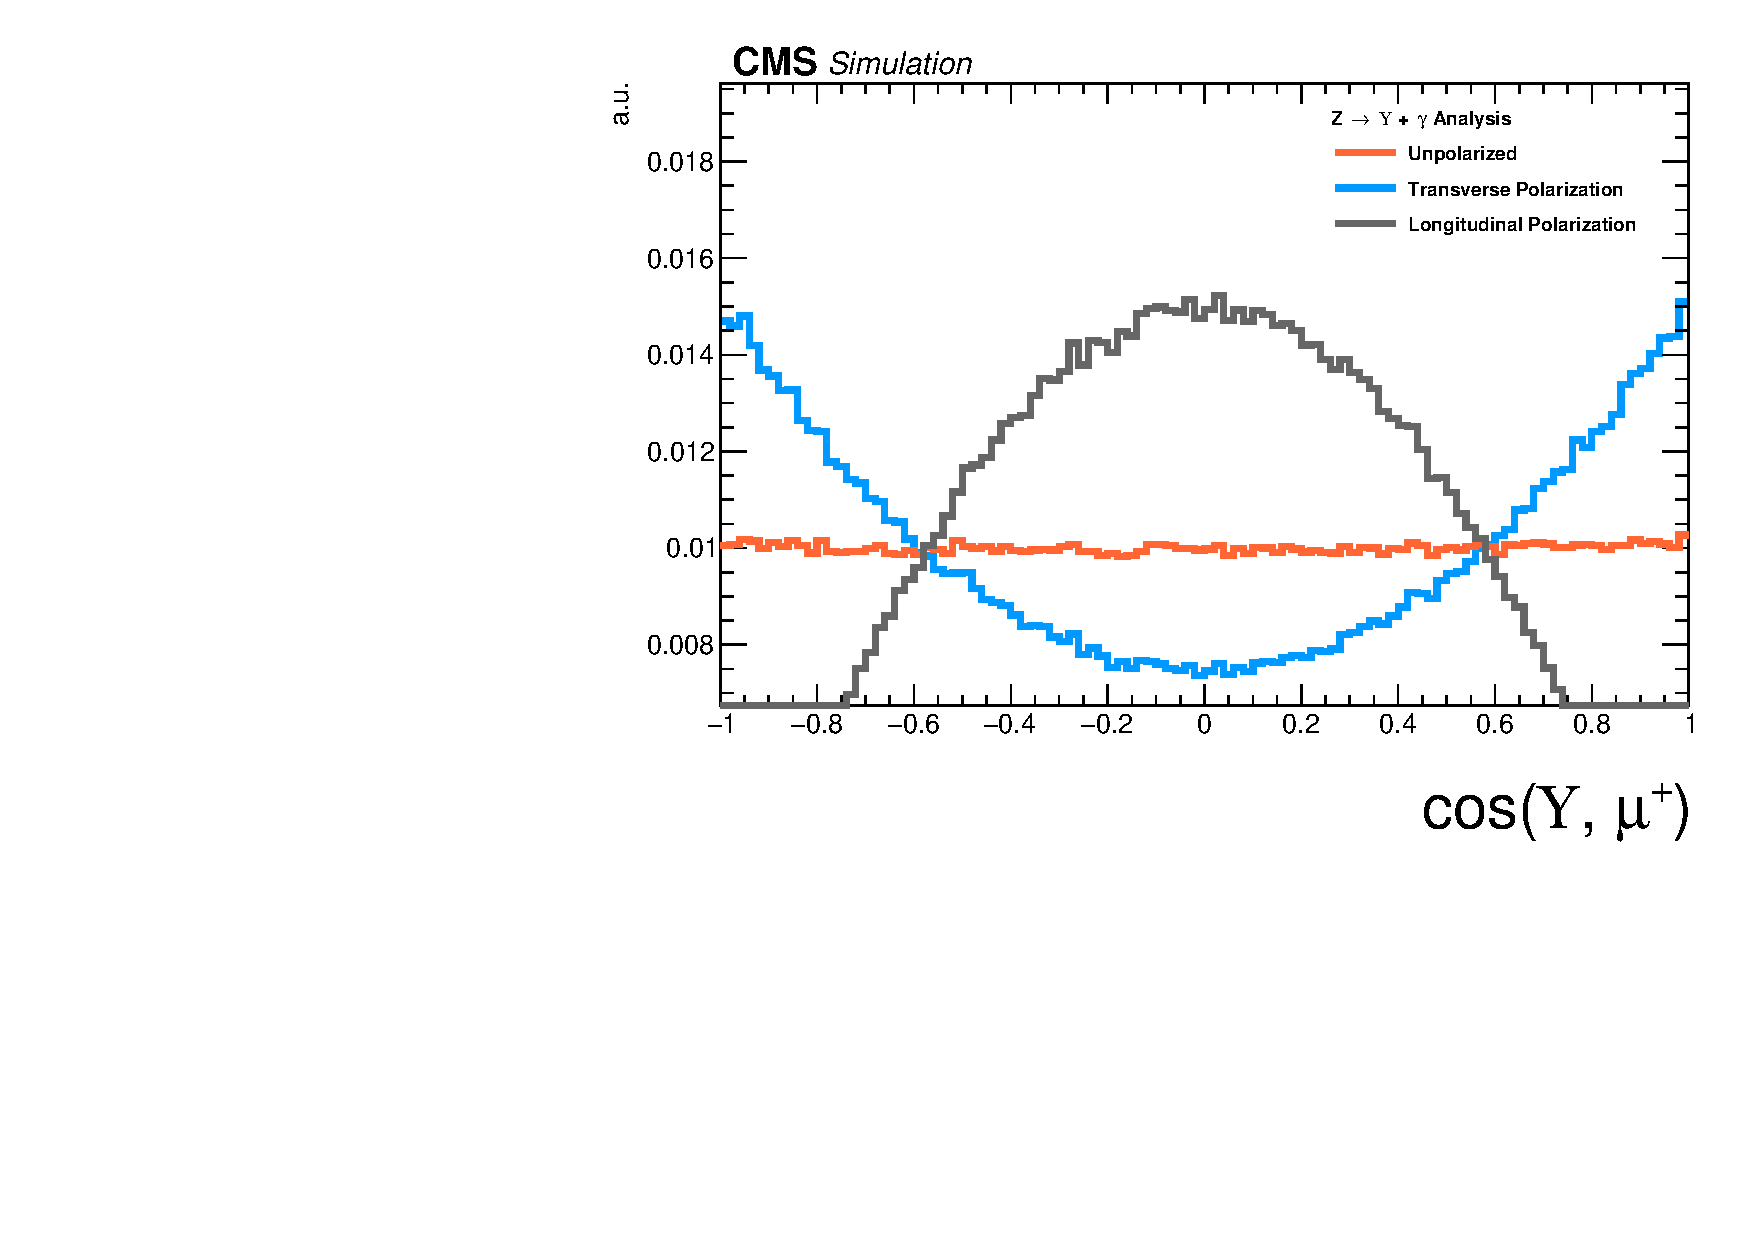
\includegraphics[width=0.80\textwidth]{figures_and_tables/outputPlots/ZtoUpsilon_Cat0_ZZZZZ/mc/polarizatioReweight/h_Gen_COS_theta_extremes}
\end{center}\vspace*{-.5cm}
\caption{Distributions of $\cos \theta$ of $\Upsilon \rightarrow \mu\mu$ and $\gamma^{*} \rightarrow \mu\mu$ The orange distribution is the $Z \rightarrow  \Upsilon(1S,2S,3S) + \gamma$ sample before reweighting (Unpolarized); the blue and gray distributions are $Z \rightarrow  \Upsilon(1S,2S,3S)$ sample after reweighting, for the Transverse and Longitudinal Polarization.}
\label{fig:ZUpsilonPolarization}
\end{figure}


\begin{table}[htp]
\begin{center}
\caption{Summary of the impact of reweighted of polarization contribution using several scenarios.}
%\begin{table}[htp]
%\begin{center}
%\begin{tabular}{|cl }
\begin{tabular}{l|l|l}

% \hline

\textbf{$J_{Z}$} & \textbf{Polarisation Scenario} & \textbf{Analytic Description} \\ \hline
$\pm$ 1  & Transverse &  3/4 $\times (1 + (\cos \Theta)^{2})$ \\ \hline
0  & Longitudinal & 3/2 $\times (1- (\cos \Theta)^{2})$ \\ 

\end{tabular}
%\caption{Summary of data samples used for $H/Z \rightarrow \Upsilon(1S,2S,3S)+\gamma$ analysis }
%\label{Tablebkg}
%\end{center}
%\end{table}
% Ref latex: https://tex.stackexchange.com/questions/112343/beautiful-table-samples


\label{fig:polTable}
\end{center}
\end{table} 



\section{Kinematical studies using MC generator}


Using the \PYTHIA 8.226 generator, the Monte Carlo signals are produced for Higgs (Z) boson events decaying into ($\Upsilon$(1S,2S,3S)) + $\gamma$, which are highly boosted. Observing the kinematic generator level distributions in Figure \ref{fig:MC_ZtoUpsilon_Cat0} for Z boson and Figure \ref{fig:MC_HtoUpsilon_Cat0} for Higgs boson, we could conclude that the high-\ET (transverse energy, with respect to the beam line) photon will be back-to-back to the $\Upsilon$ particles being possible to apply an isolation selection to identify a photon in this kinematic topology. Also, we can observe those transverse momenta of the leading/trailing \PT (transverse momemtum, with respect to the beam line) muon~\footnote{In this study we define leading muon and the muon, decaying from the $\Upsilon$, with highest \PT. Trailing muon is the one with the second hight \PT.} and the photon and distances $\Delta R=\sqrt{\Delta\eta^2 + \Delta\phi^2}$ between the two muons and between the muons and the photon are a good variable that can be used to discriminate the contribution between signal and background events. The leading muon transverse momentum can be greater than 45(30)\GeV and trailing muon is greater than 10(20)\GeV in Higgs(Z) decay. $\Delta R$ distributions of the two muons and between the muons and the photon in the both cases show that the two muons are very close and the photon is back-to-back in relation of dimuon system. Another feature of this kinematic topology is that the production vertex between muons produced in $\Upsilon$ decaying events and the high-\ET photon is measured with high precision.  

it is worth to mention that discussion above is made only on simulated data samples for this analysis and does not necessarily translate to the real data analysis without further inspection.

% Concerning the main reducible background (combinatorial background), it is due to Drell-Yan process where the photon comes from the initial-state radiation (ISR) or final-state radiation (FSR) and background reducible events are produced from Drell-Yan with jet associate and inclusive quarkonium production, where the jet in both processes is misidentified as a photon in reconstruction level. For the analysis, besides the resonant background, most of the background contributions will be modeled from data. 

\begin{figure}[!htbp]
\begin{center}
% Muon
%\hspace*{1.cm}
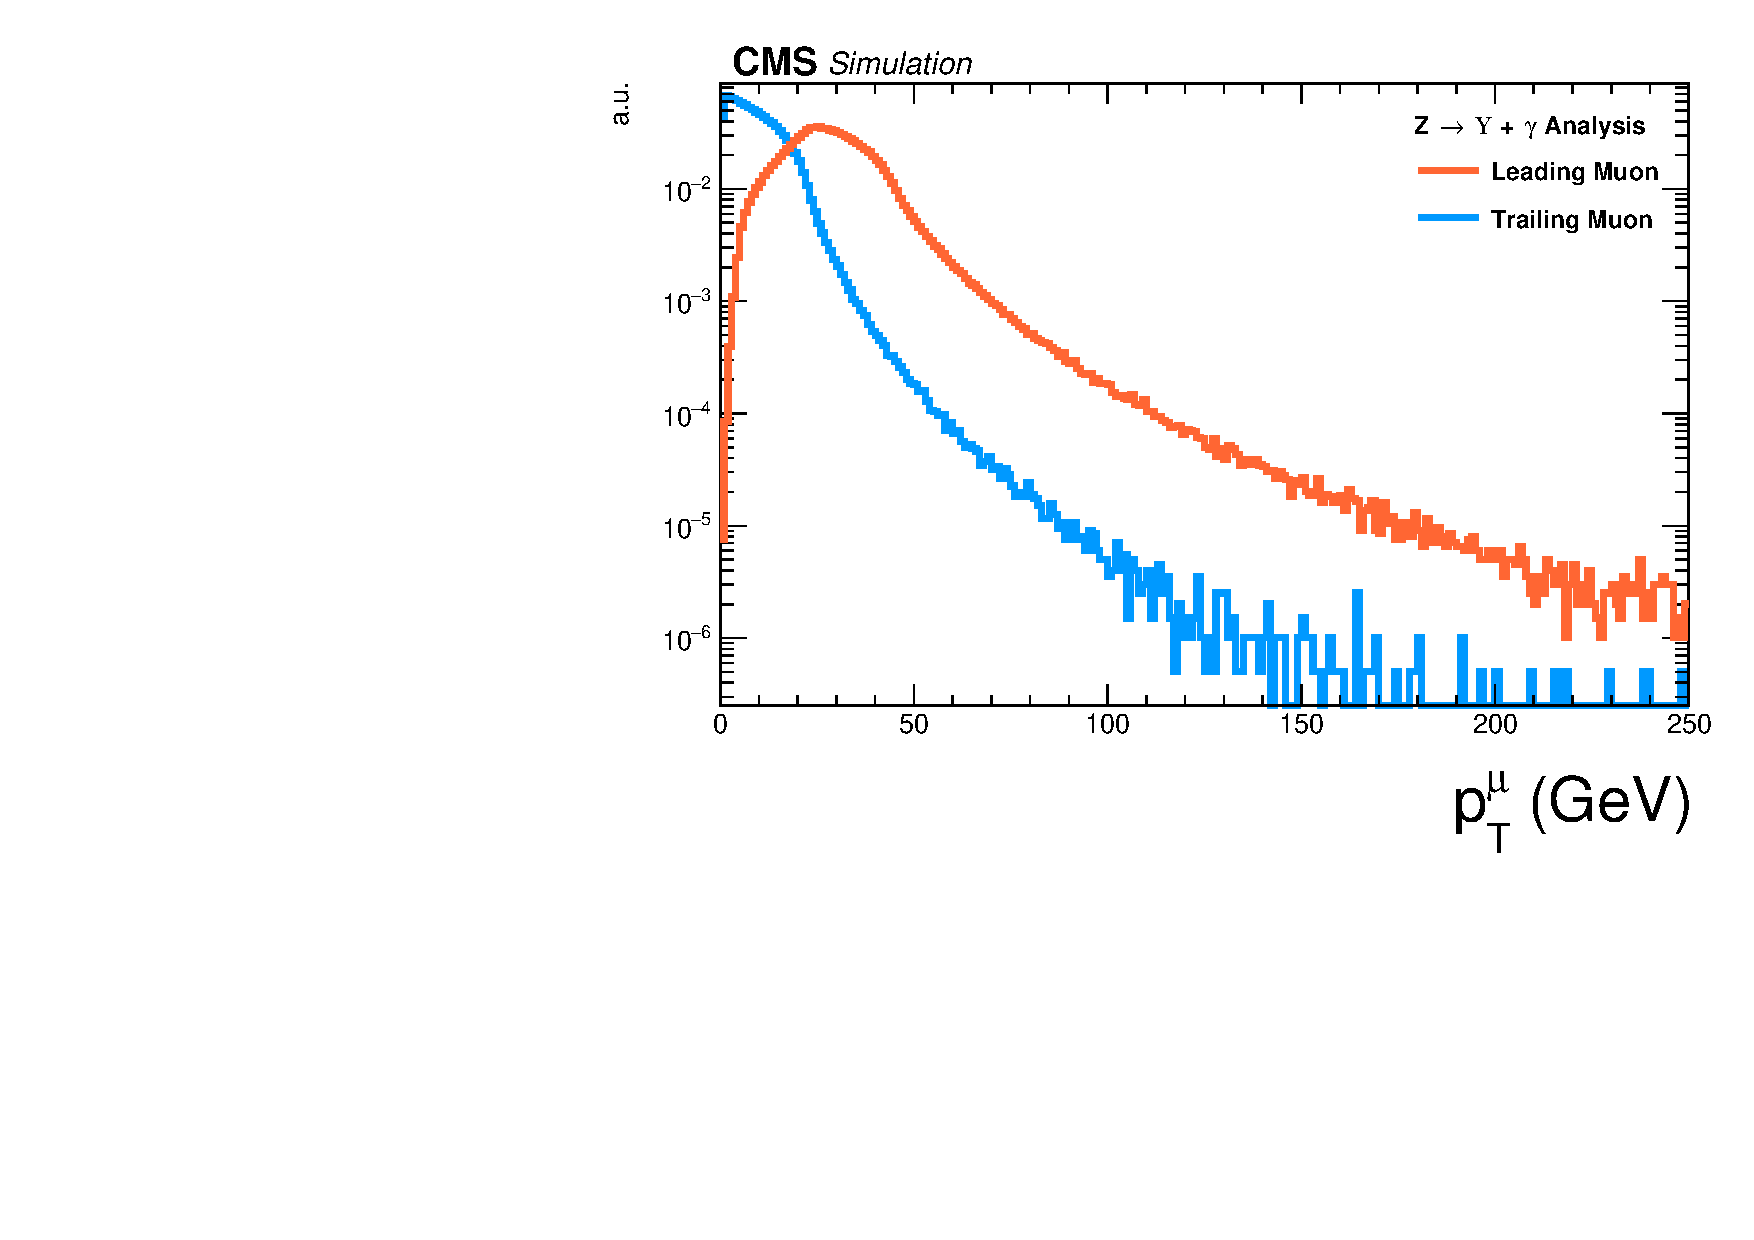
\includegraphics[width=0.45\textwidth]{figures_and_tables/outputPlots/ZtoUpsilon_Cat0_ZZZZZ/mc/unpolarized/h_Gen_Mu_pt}
%\hspace*{1.cm}
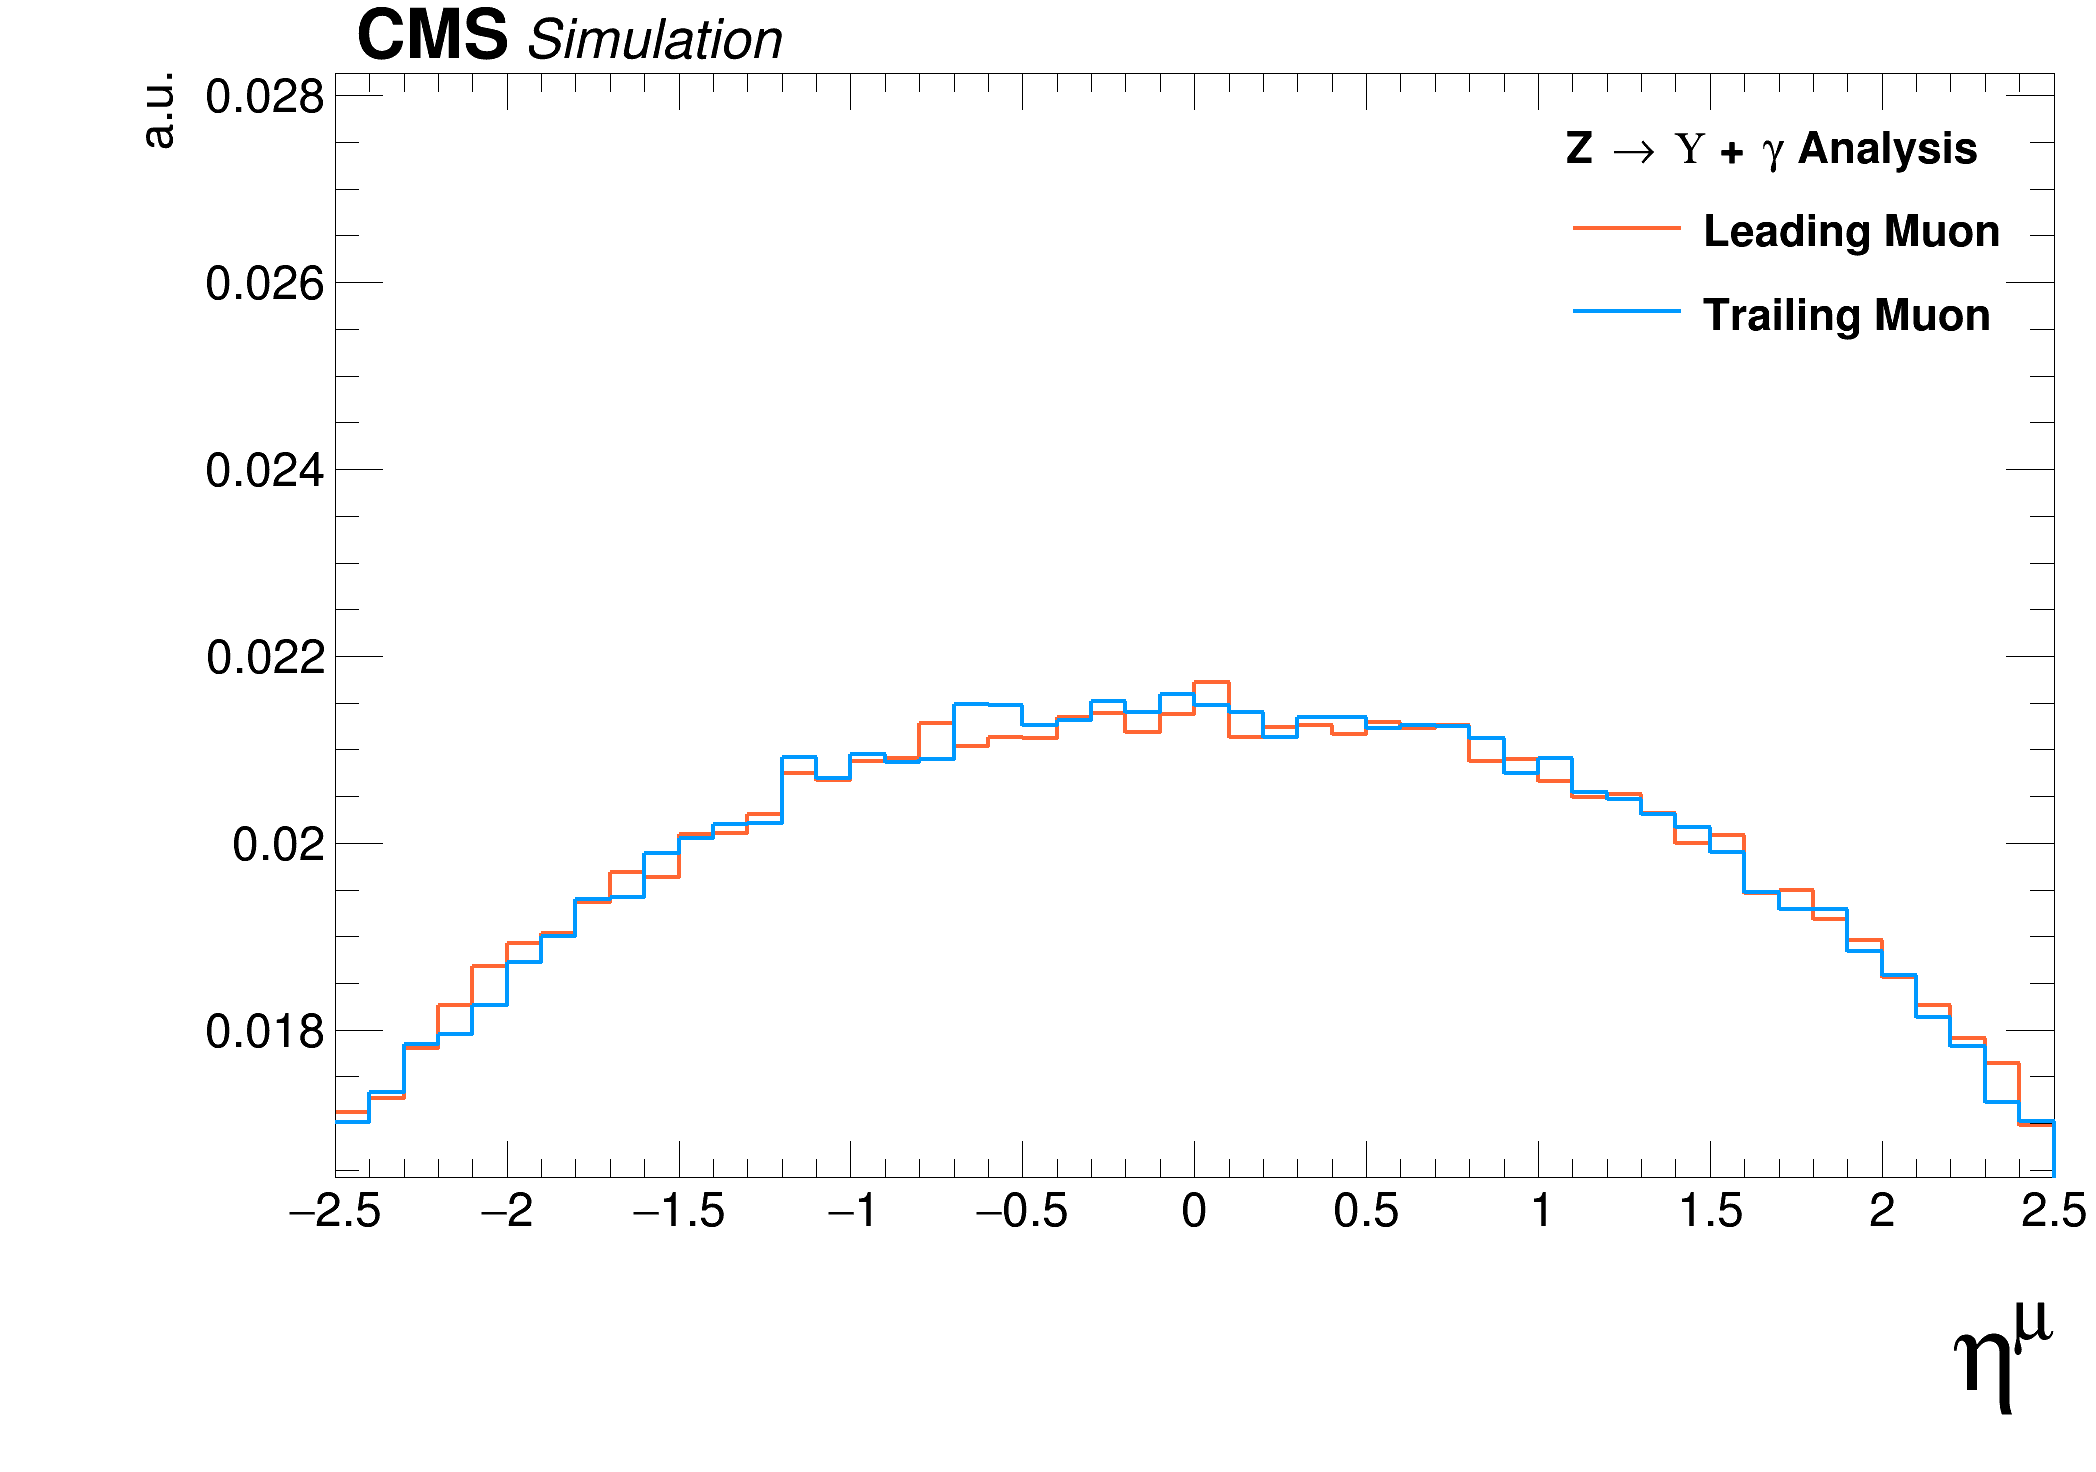
\includegraphics[width=0.45\textwidth]{figures_and_tables/outputPlots/ZtoUpsilon_Cat0_ZZZZZ/mc/unpolarized/h_Gen_Mu_eta}
%\hspace*{1.cm}
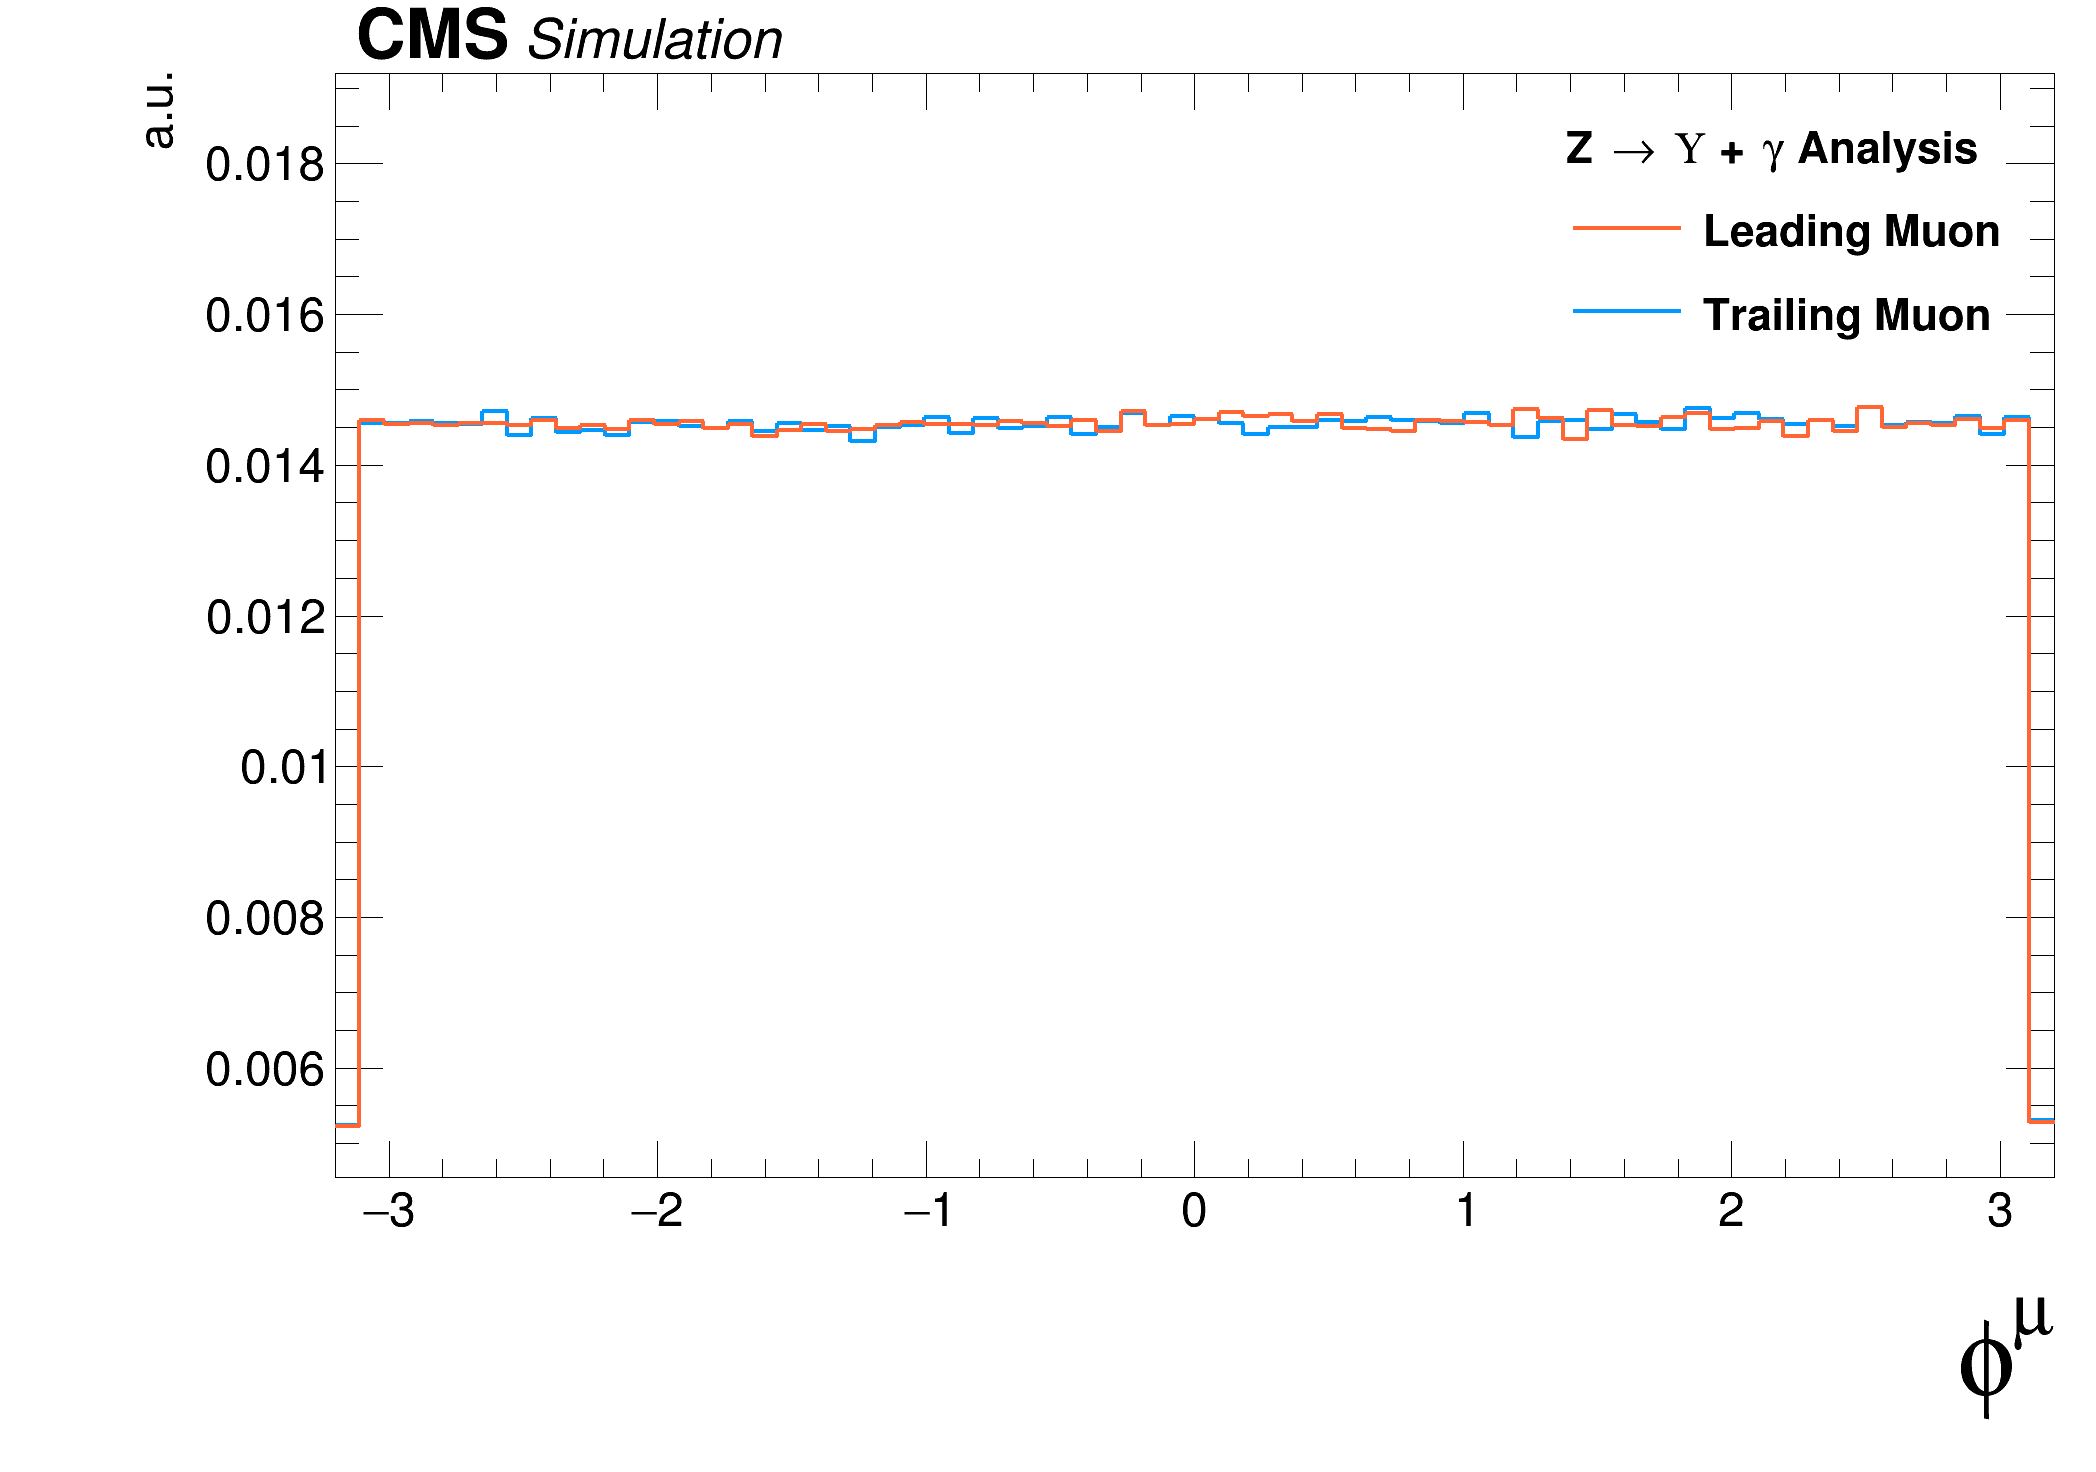
\includegraphics[width=0.45\textwidth]{figures_and_tables/outputPlots/ZtoUpsilon_Cat0_ZZZZZ/mc/unpolarized/h_Gen_Mu_phi}
%\hspace*{1.cm}
%Delta R mu_trading and mu_leading
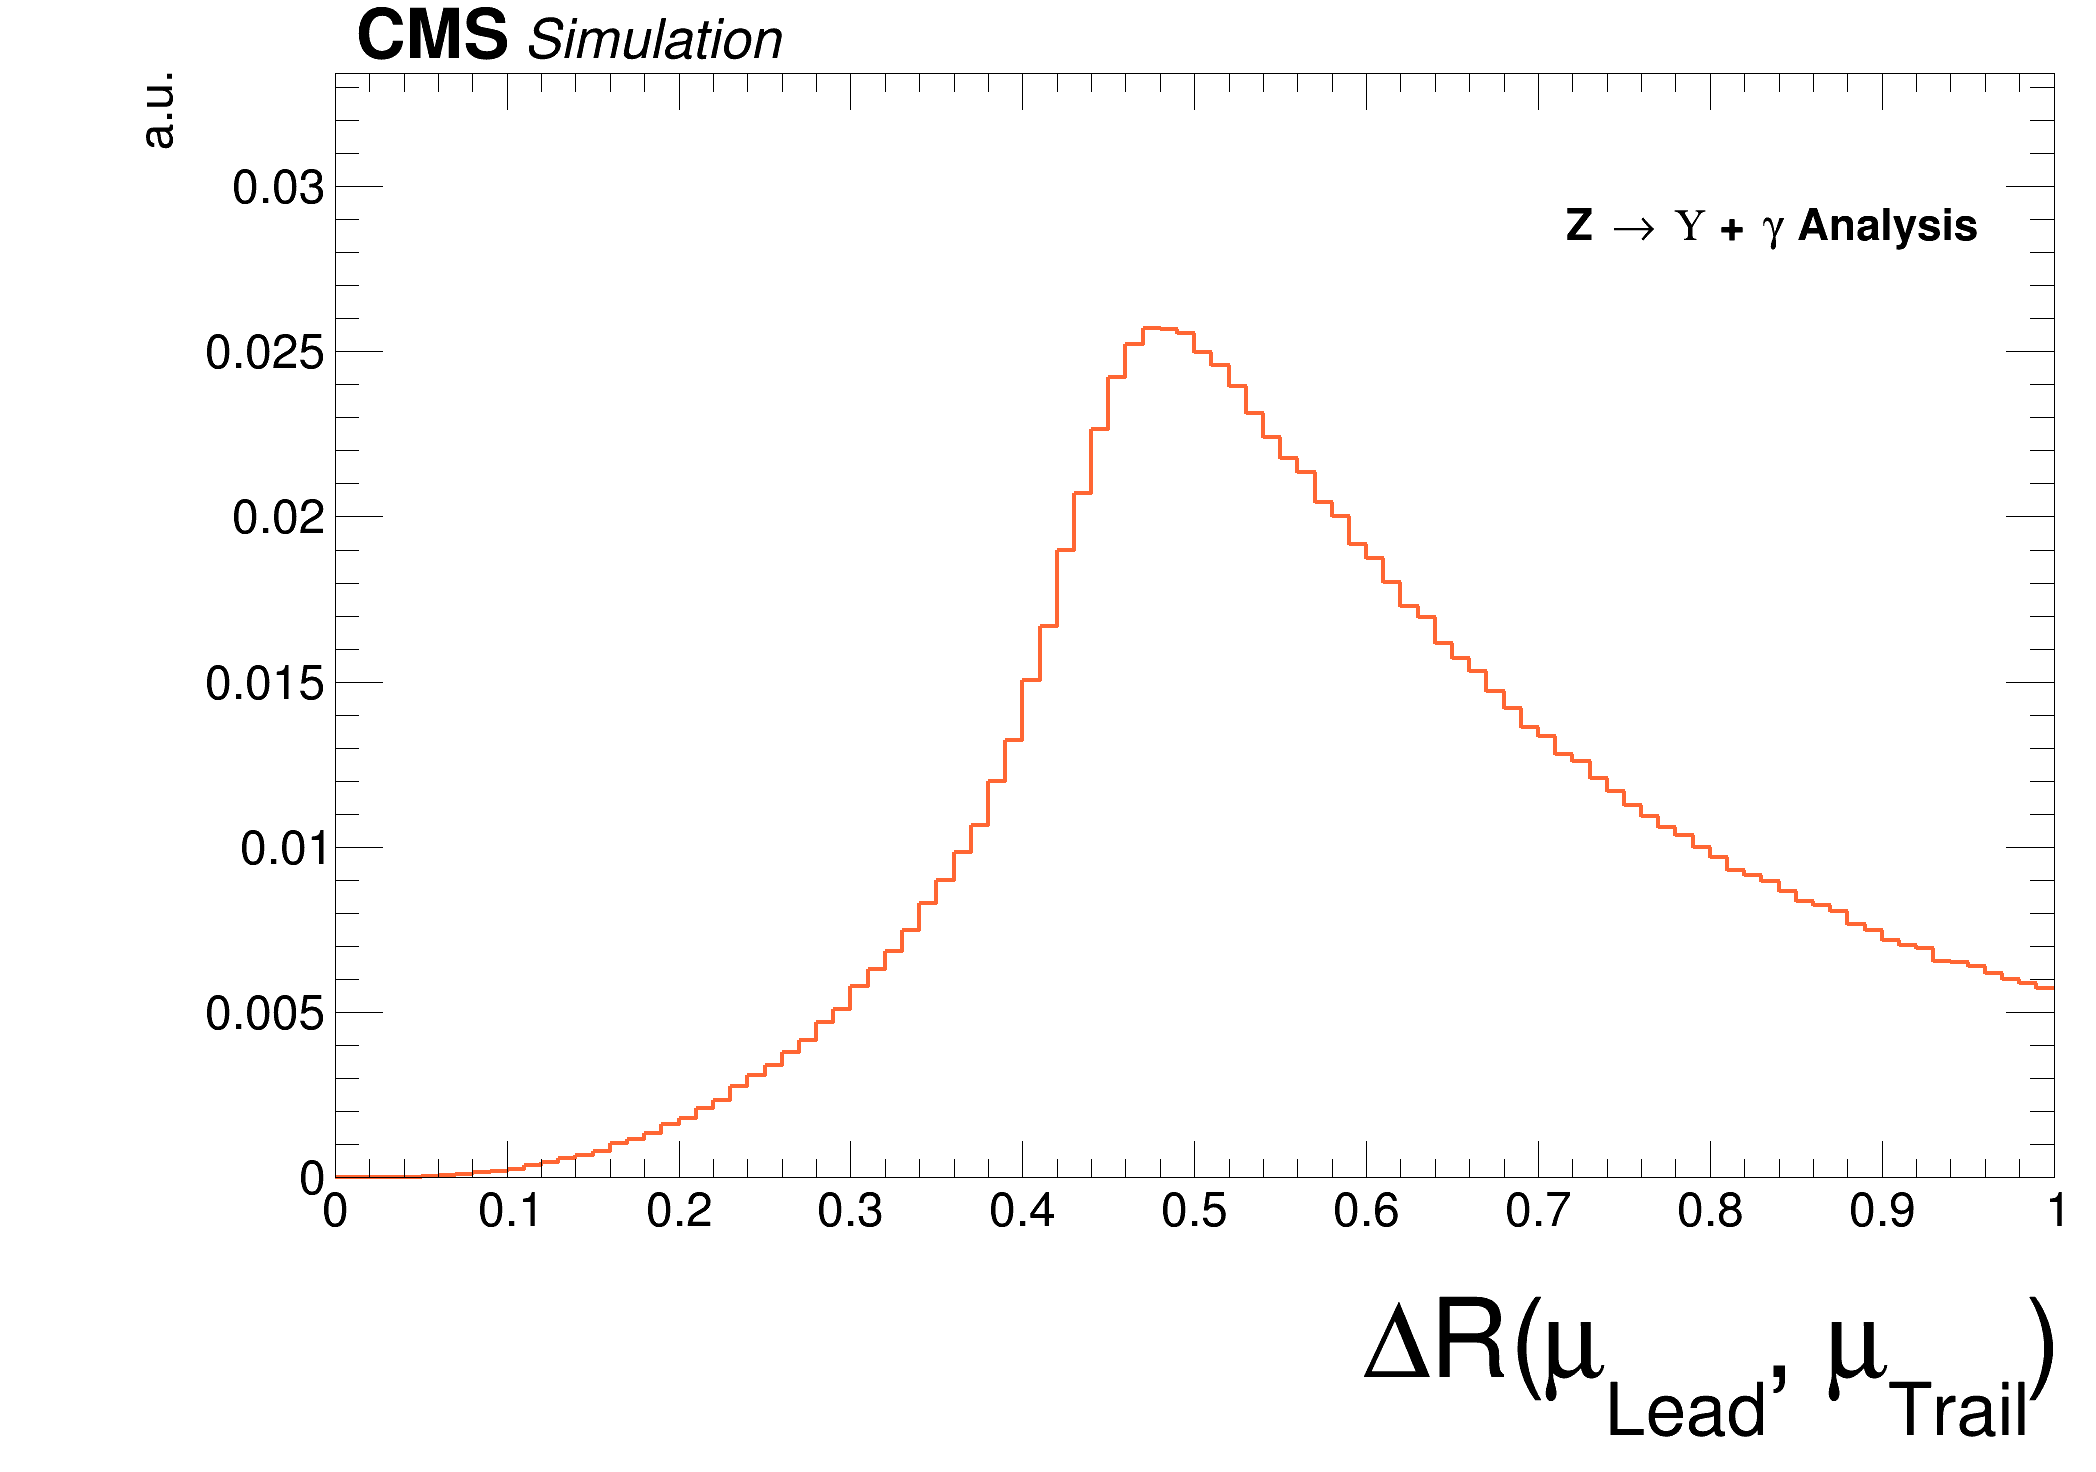
\includegraphics[width=0.45\textwidth]{figures_and_tables/outputPlots/ZtoUpsilon_Cat0_ZZZZZ/mc/unpolarized/h_Gen_deltaR_Leading_Trailing}
%\hspace*{1.cm}
%Photon
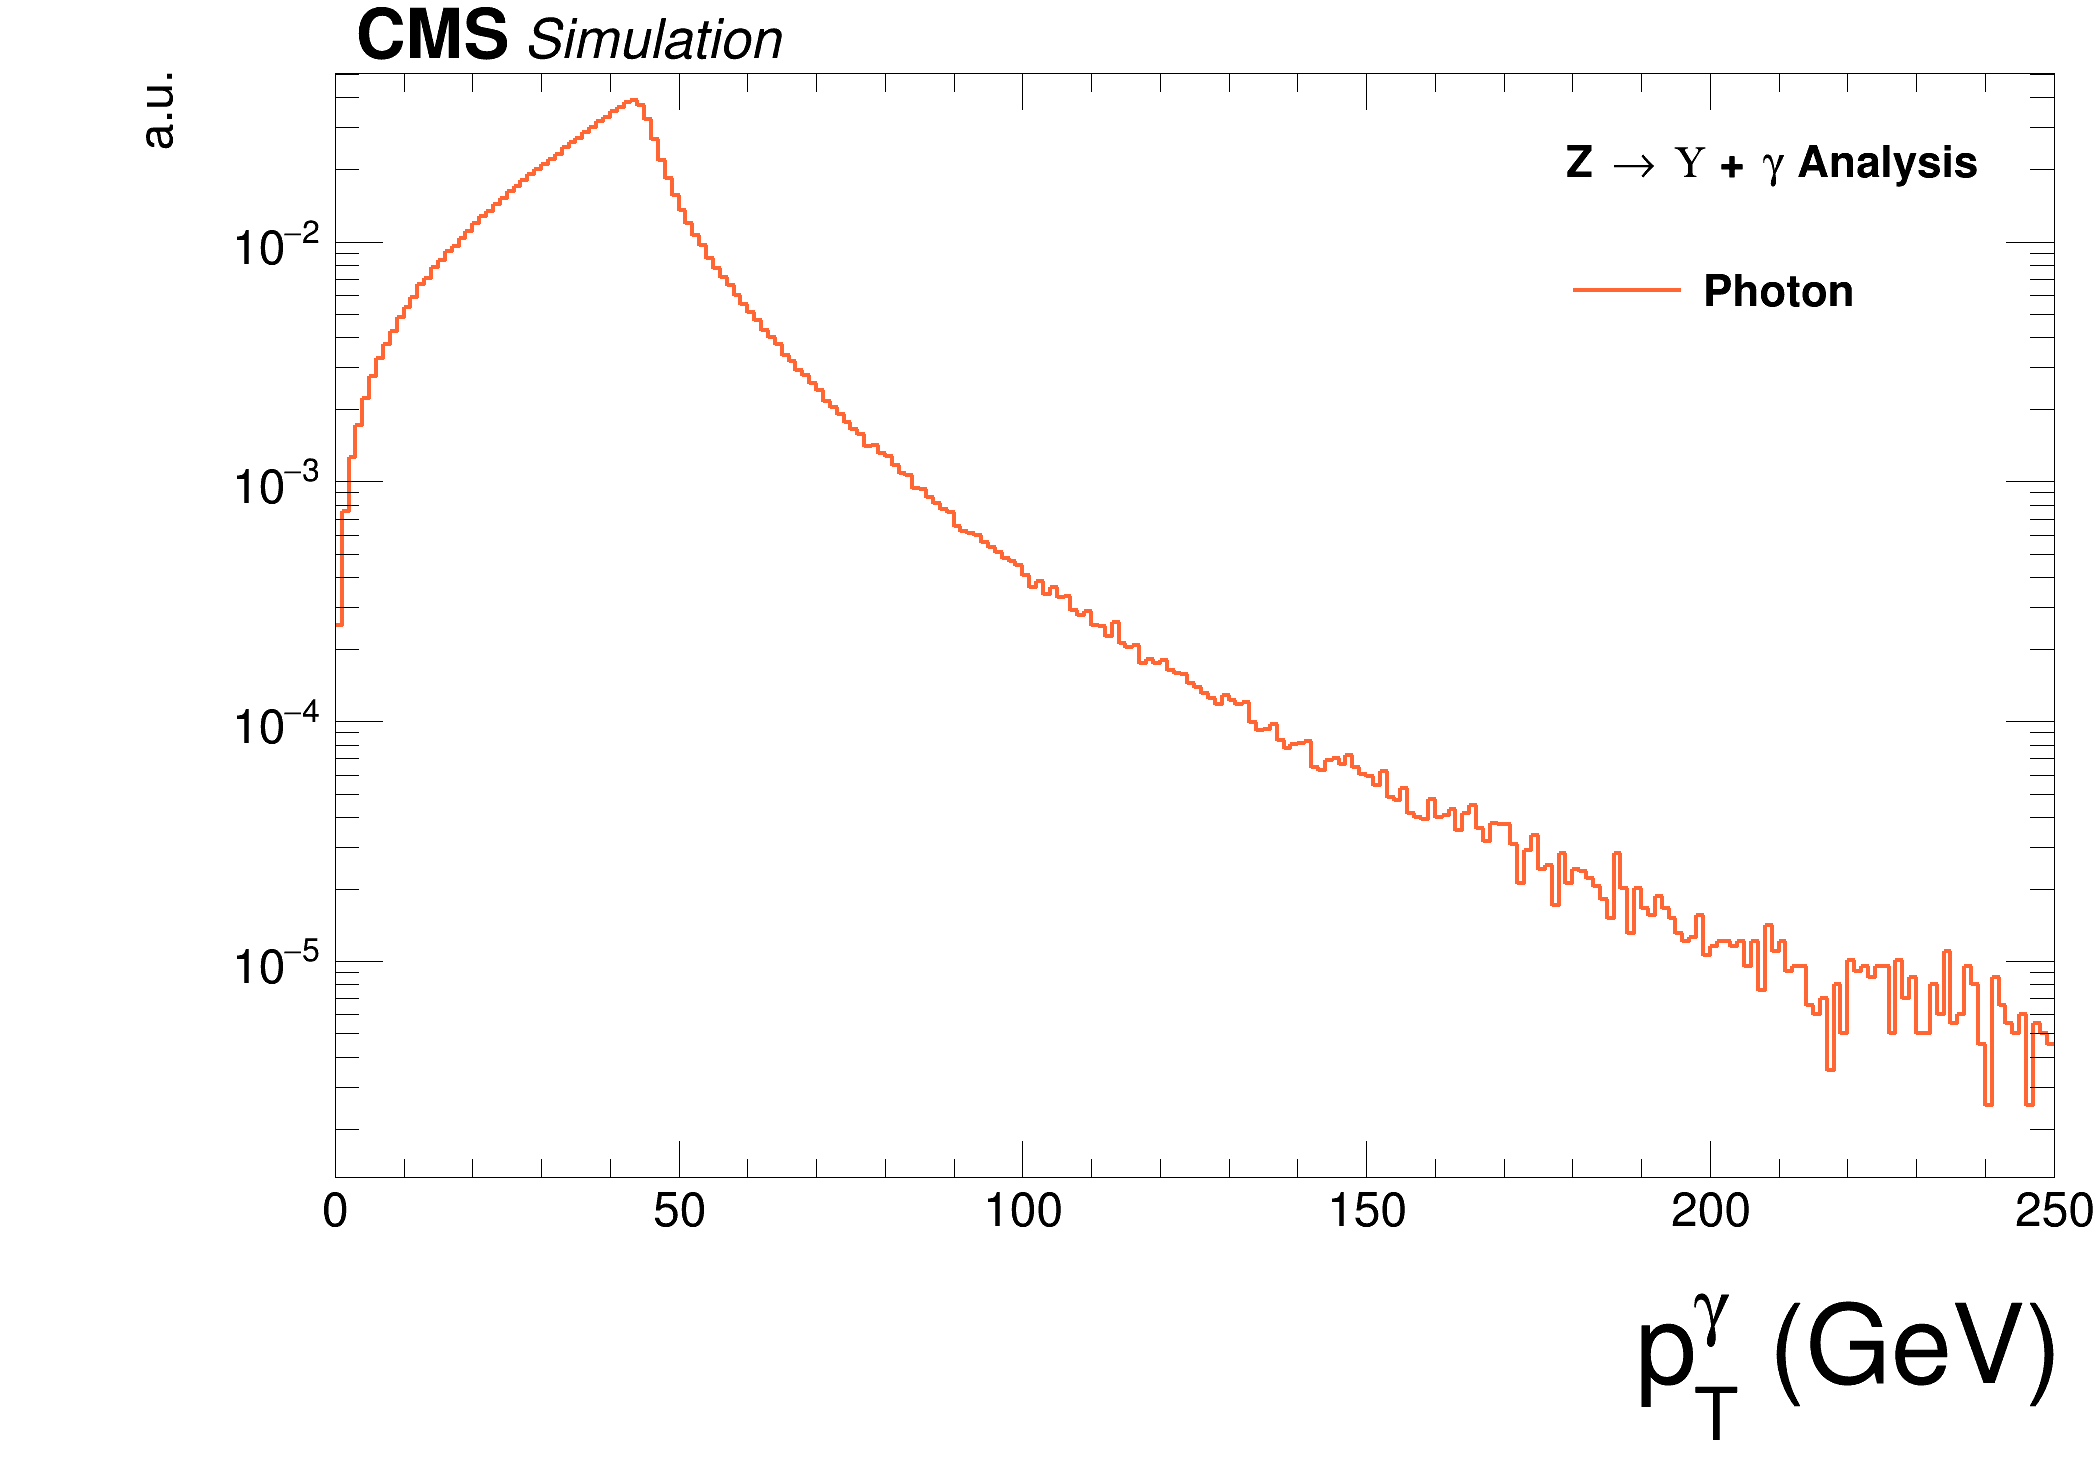
\includegraphics[width=0.45\textwidth]{figures_and_tables/outputPlots/ZtoUpsilon_Cat0_ZZZZZ/mc/unpolarized/h_Gen_Photon_pt}
%\hspace*{1.cm}
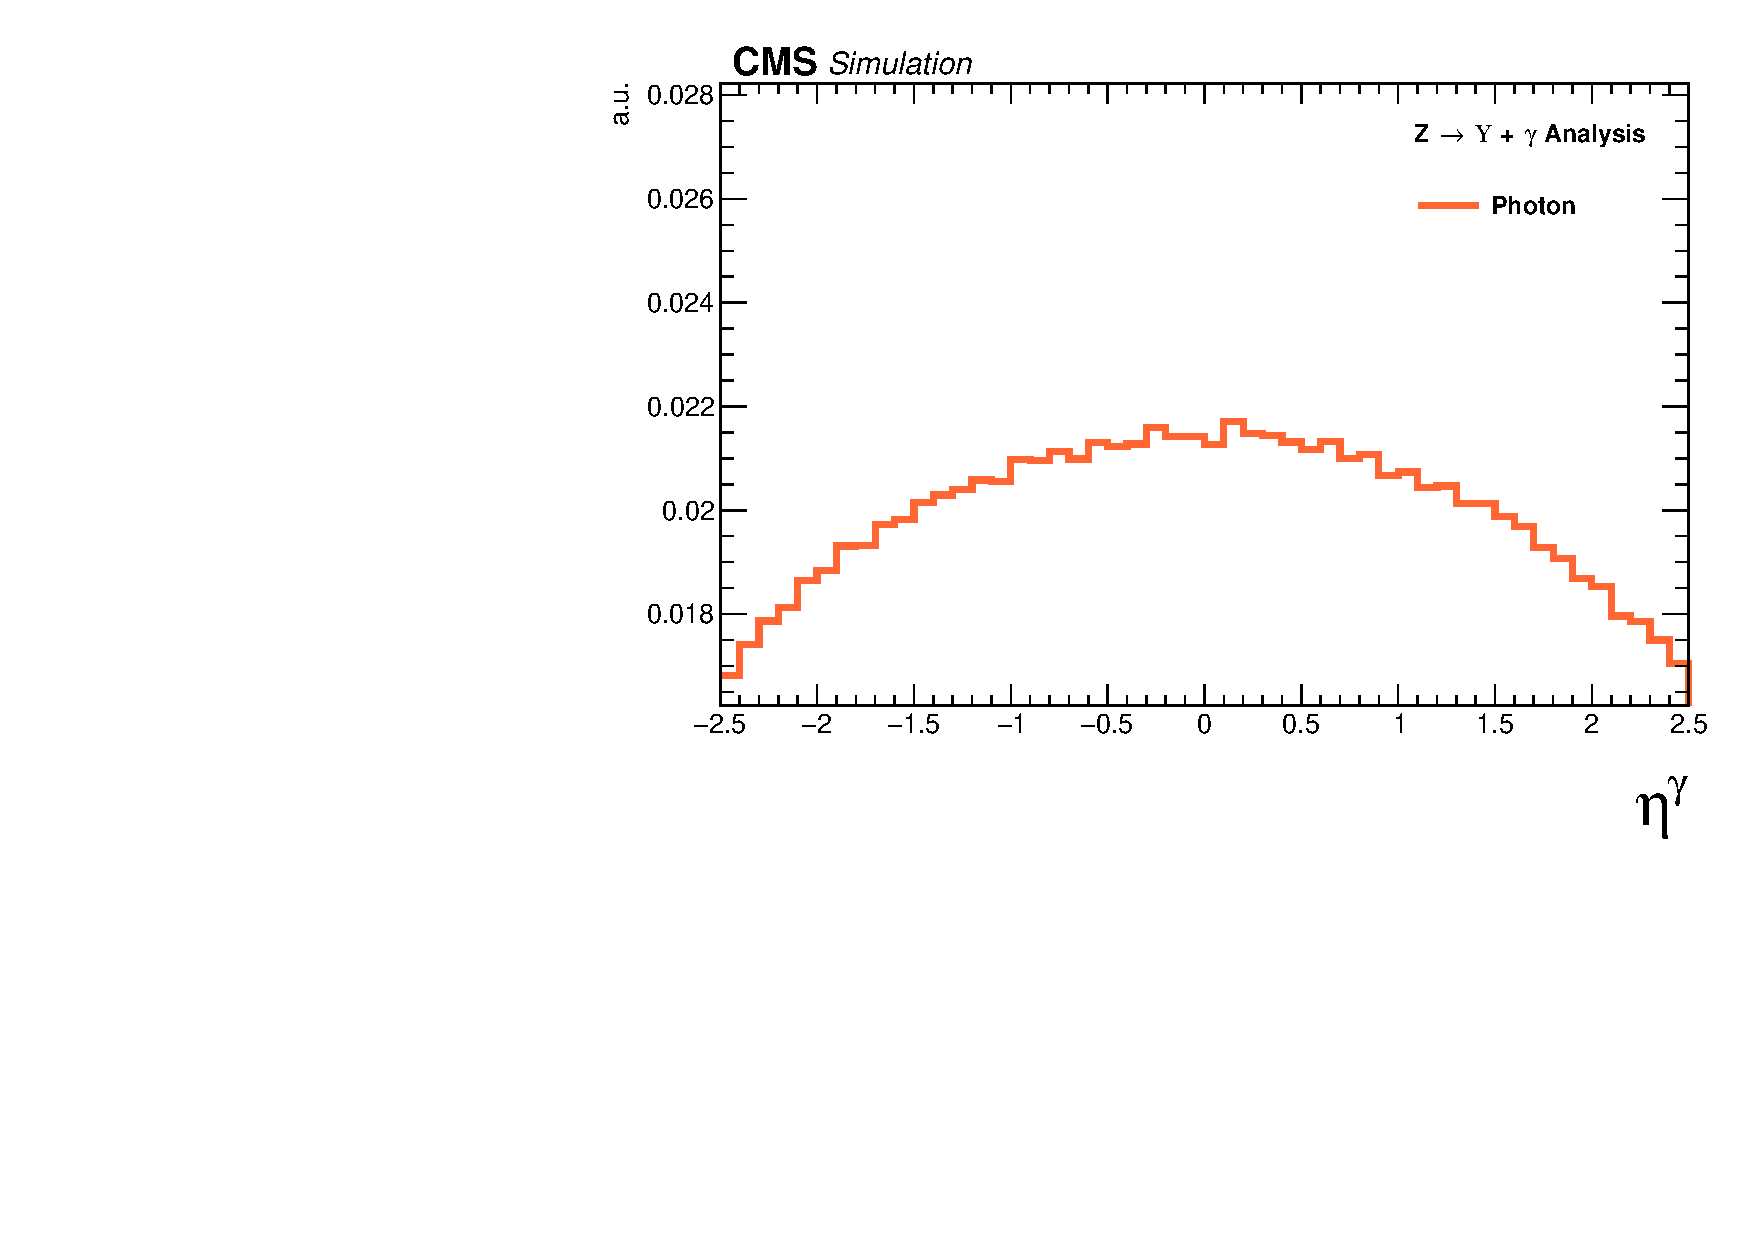
\includegraphics[width=0.45\textwidth]{figures_and_tables/outputPlots/ZtoUpsilon_Cat0_ZZZZZ/mc/unpolarized/h_Gen_Photon_eta}
%\hspace*{1.cm}
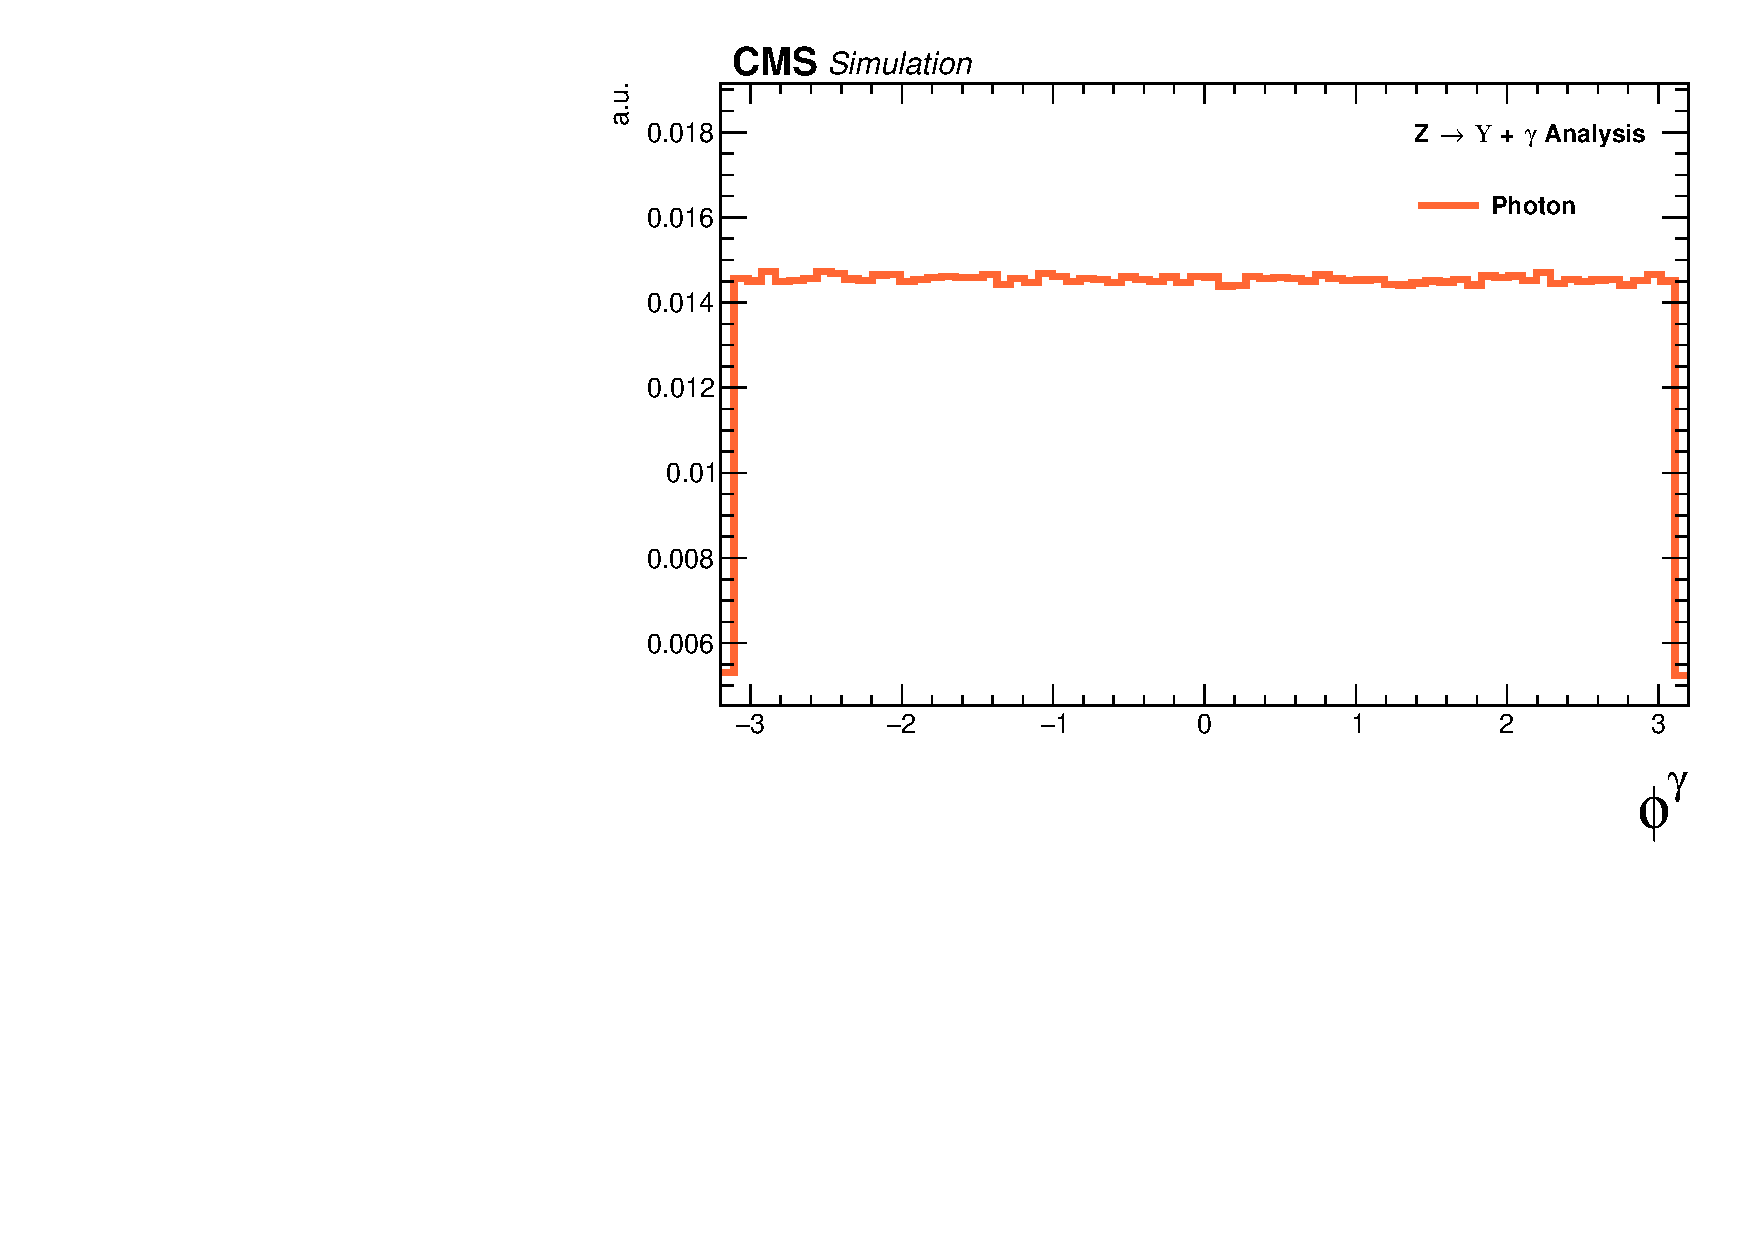
\includegraphics[width=0.45\textwidth]{figures_and_tables/outputPlots/ZtoUpsilon_Cat0_ZZZZZ/mc/unpolarized/h_Gen_Photon_phi}
%\hspace*{1.cm}
%Delta R mu+ photon
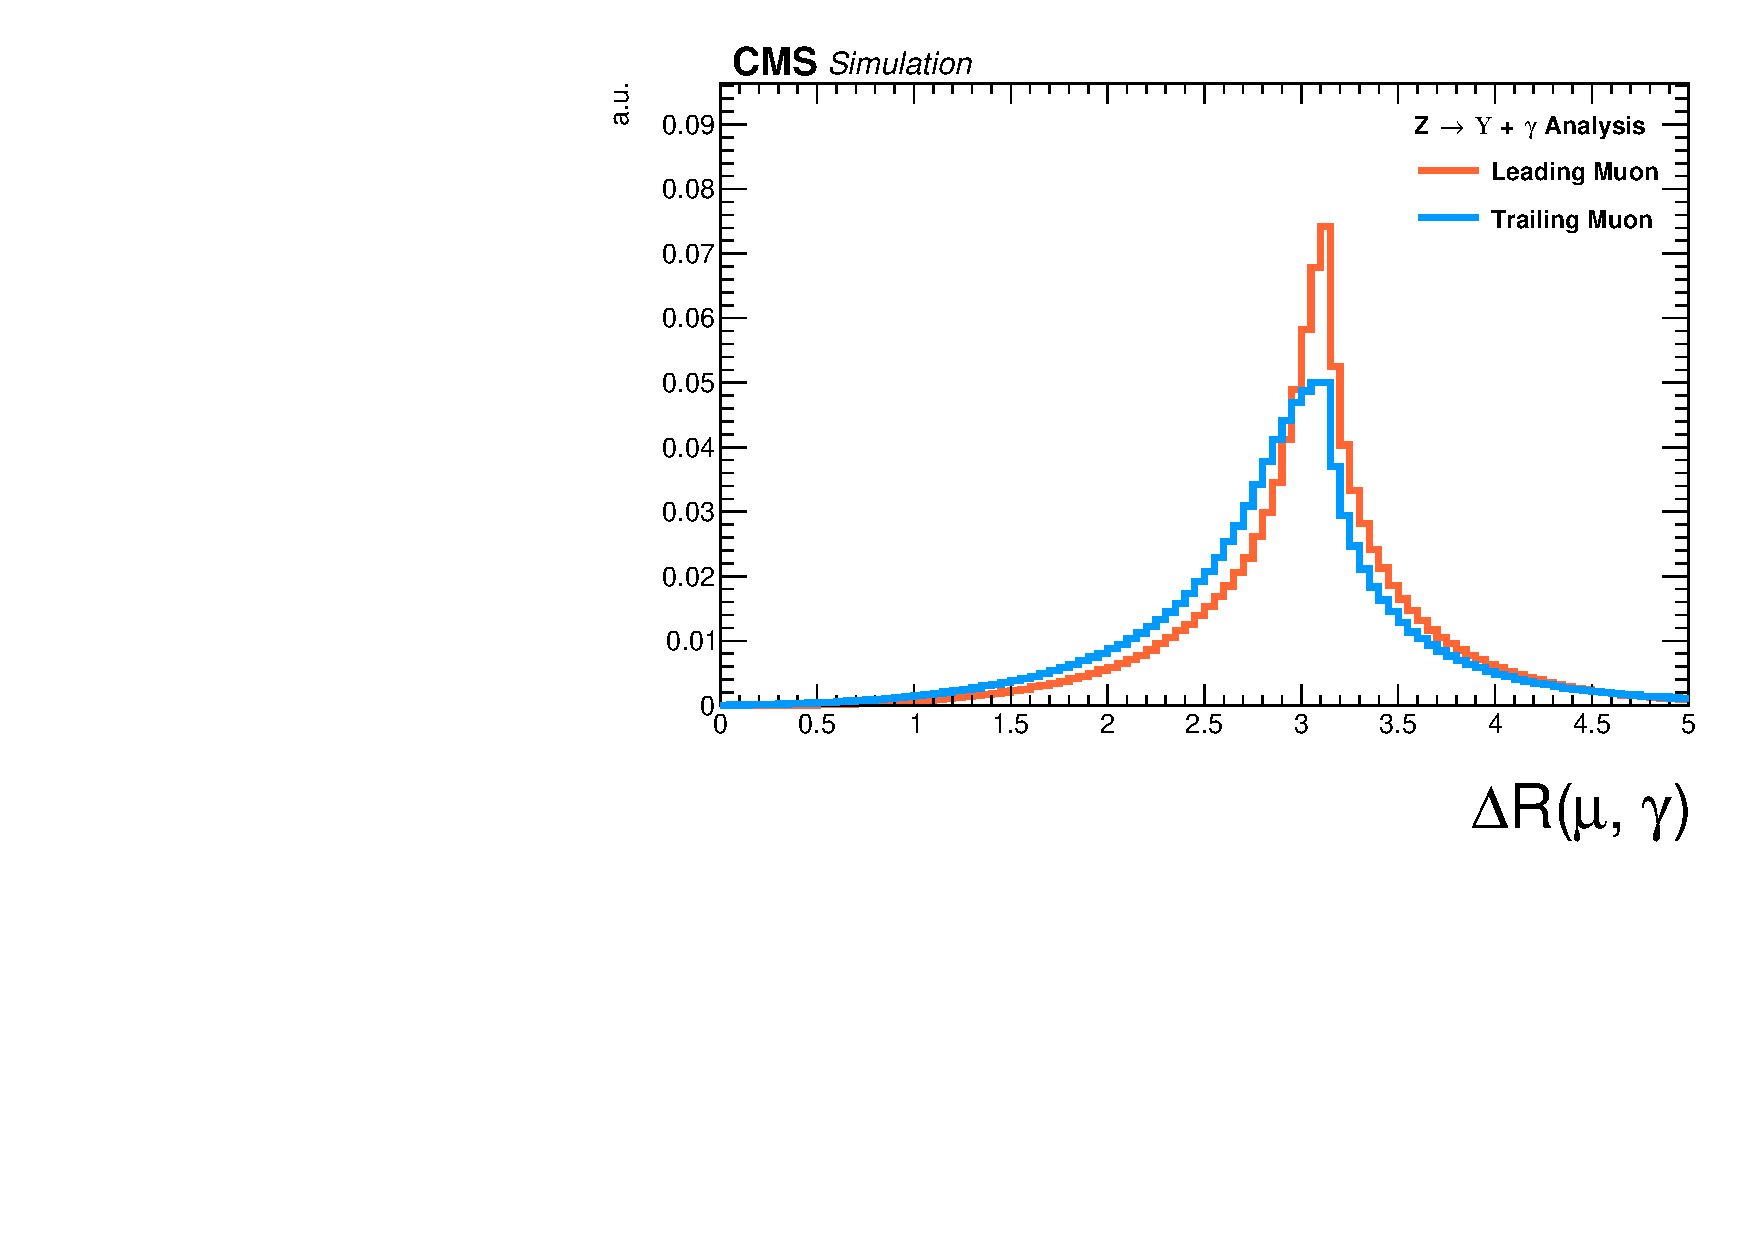
\includegraphics[width=0.45\textwidth]{figures_and_tables/outputPlots/ZtoUpsilon_Cat0_ZZZZZ/mc/unpolarized/h_Gen_deltaR_Mu_Photon}
%\hspace*{1.cm}
%Upsilon
%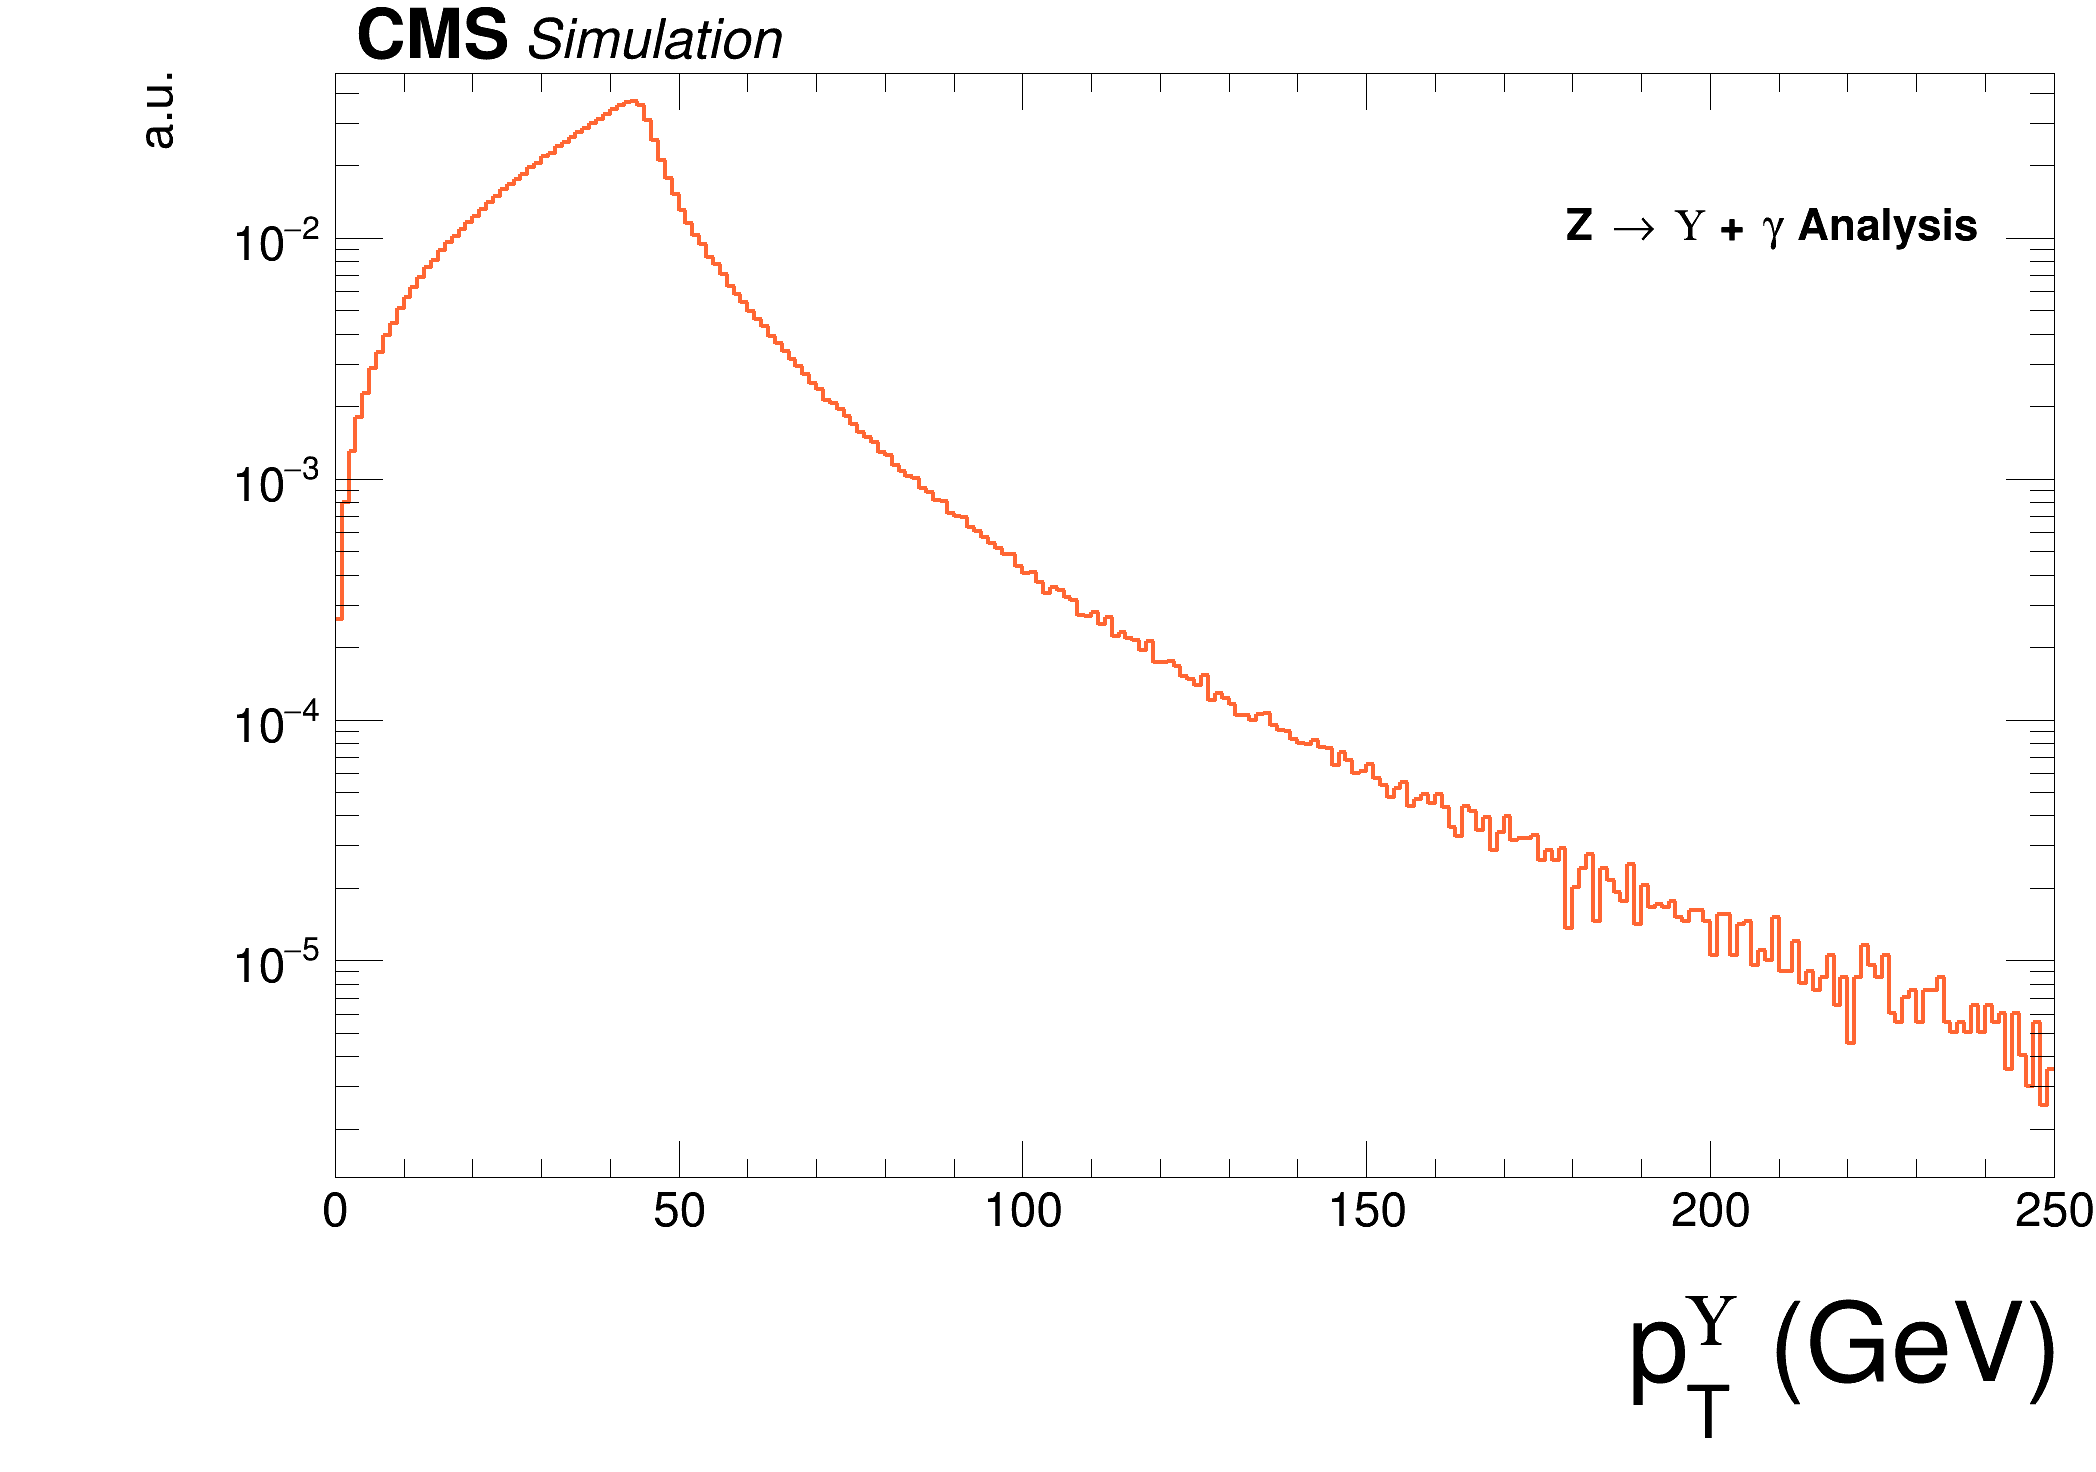
\includegraphics[width=0.25\textwidth]{figures_and_tables/outputPlots/ZtoUpsilon_Cat0_ZZZZZ/mc/unpolarized/h_Gen_Upsilon_Pt}
%\hspace*{1.cm}
%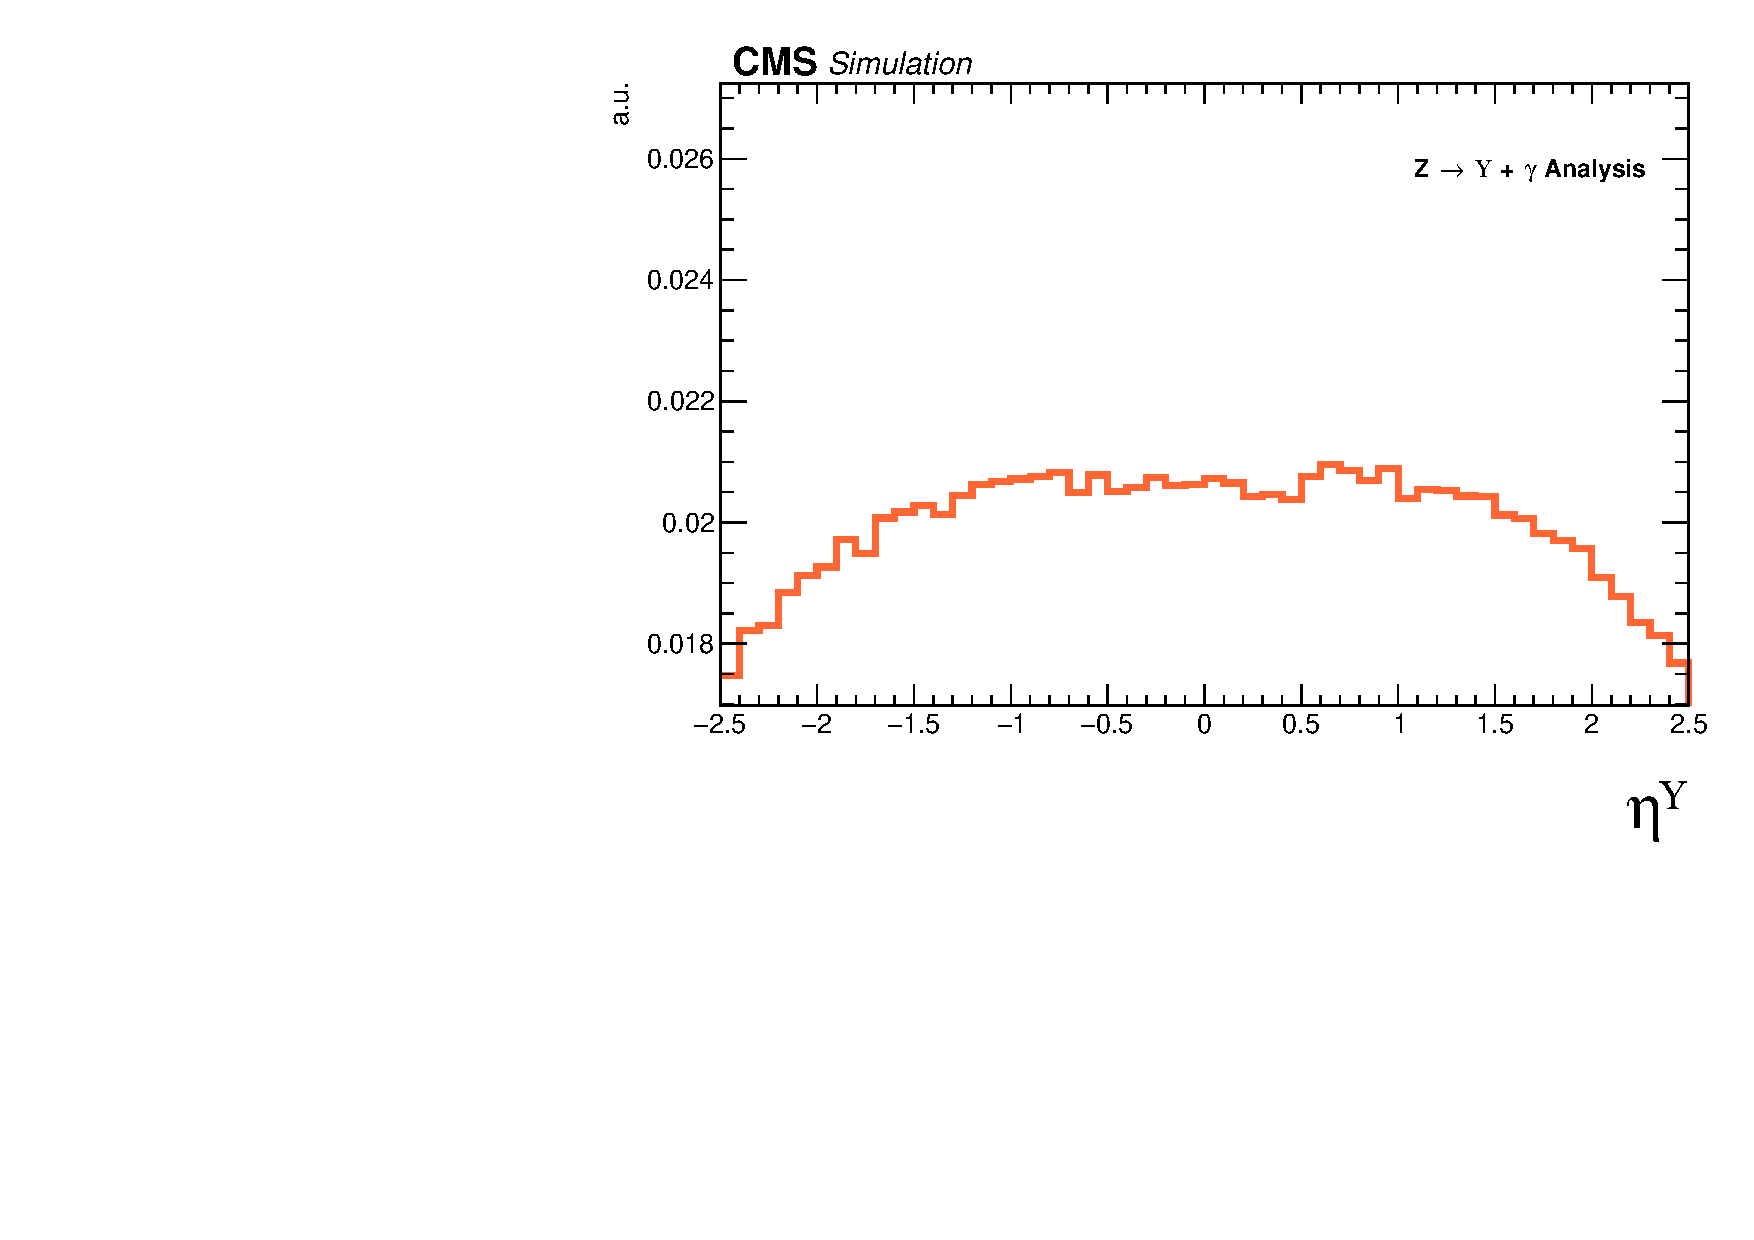
\includegraphics[width=0.25\textwidth]{figures_and_tables/outputPlots/ZtoUpsilon_Cat0_ZZZZZ/mc/unpolarized/h_Gen_Upsilon_eta}
%\hspace*{1.cm}
%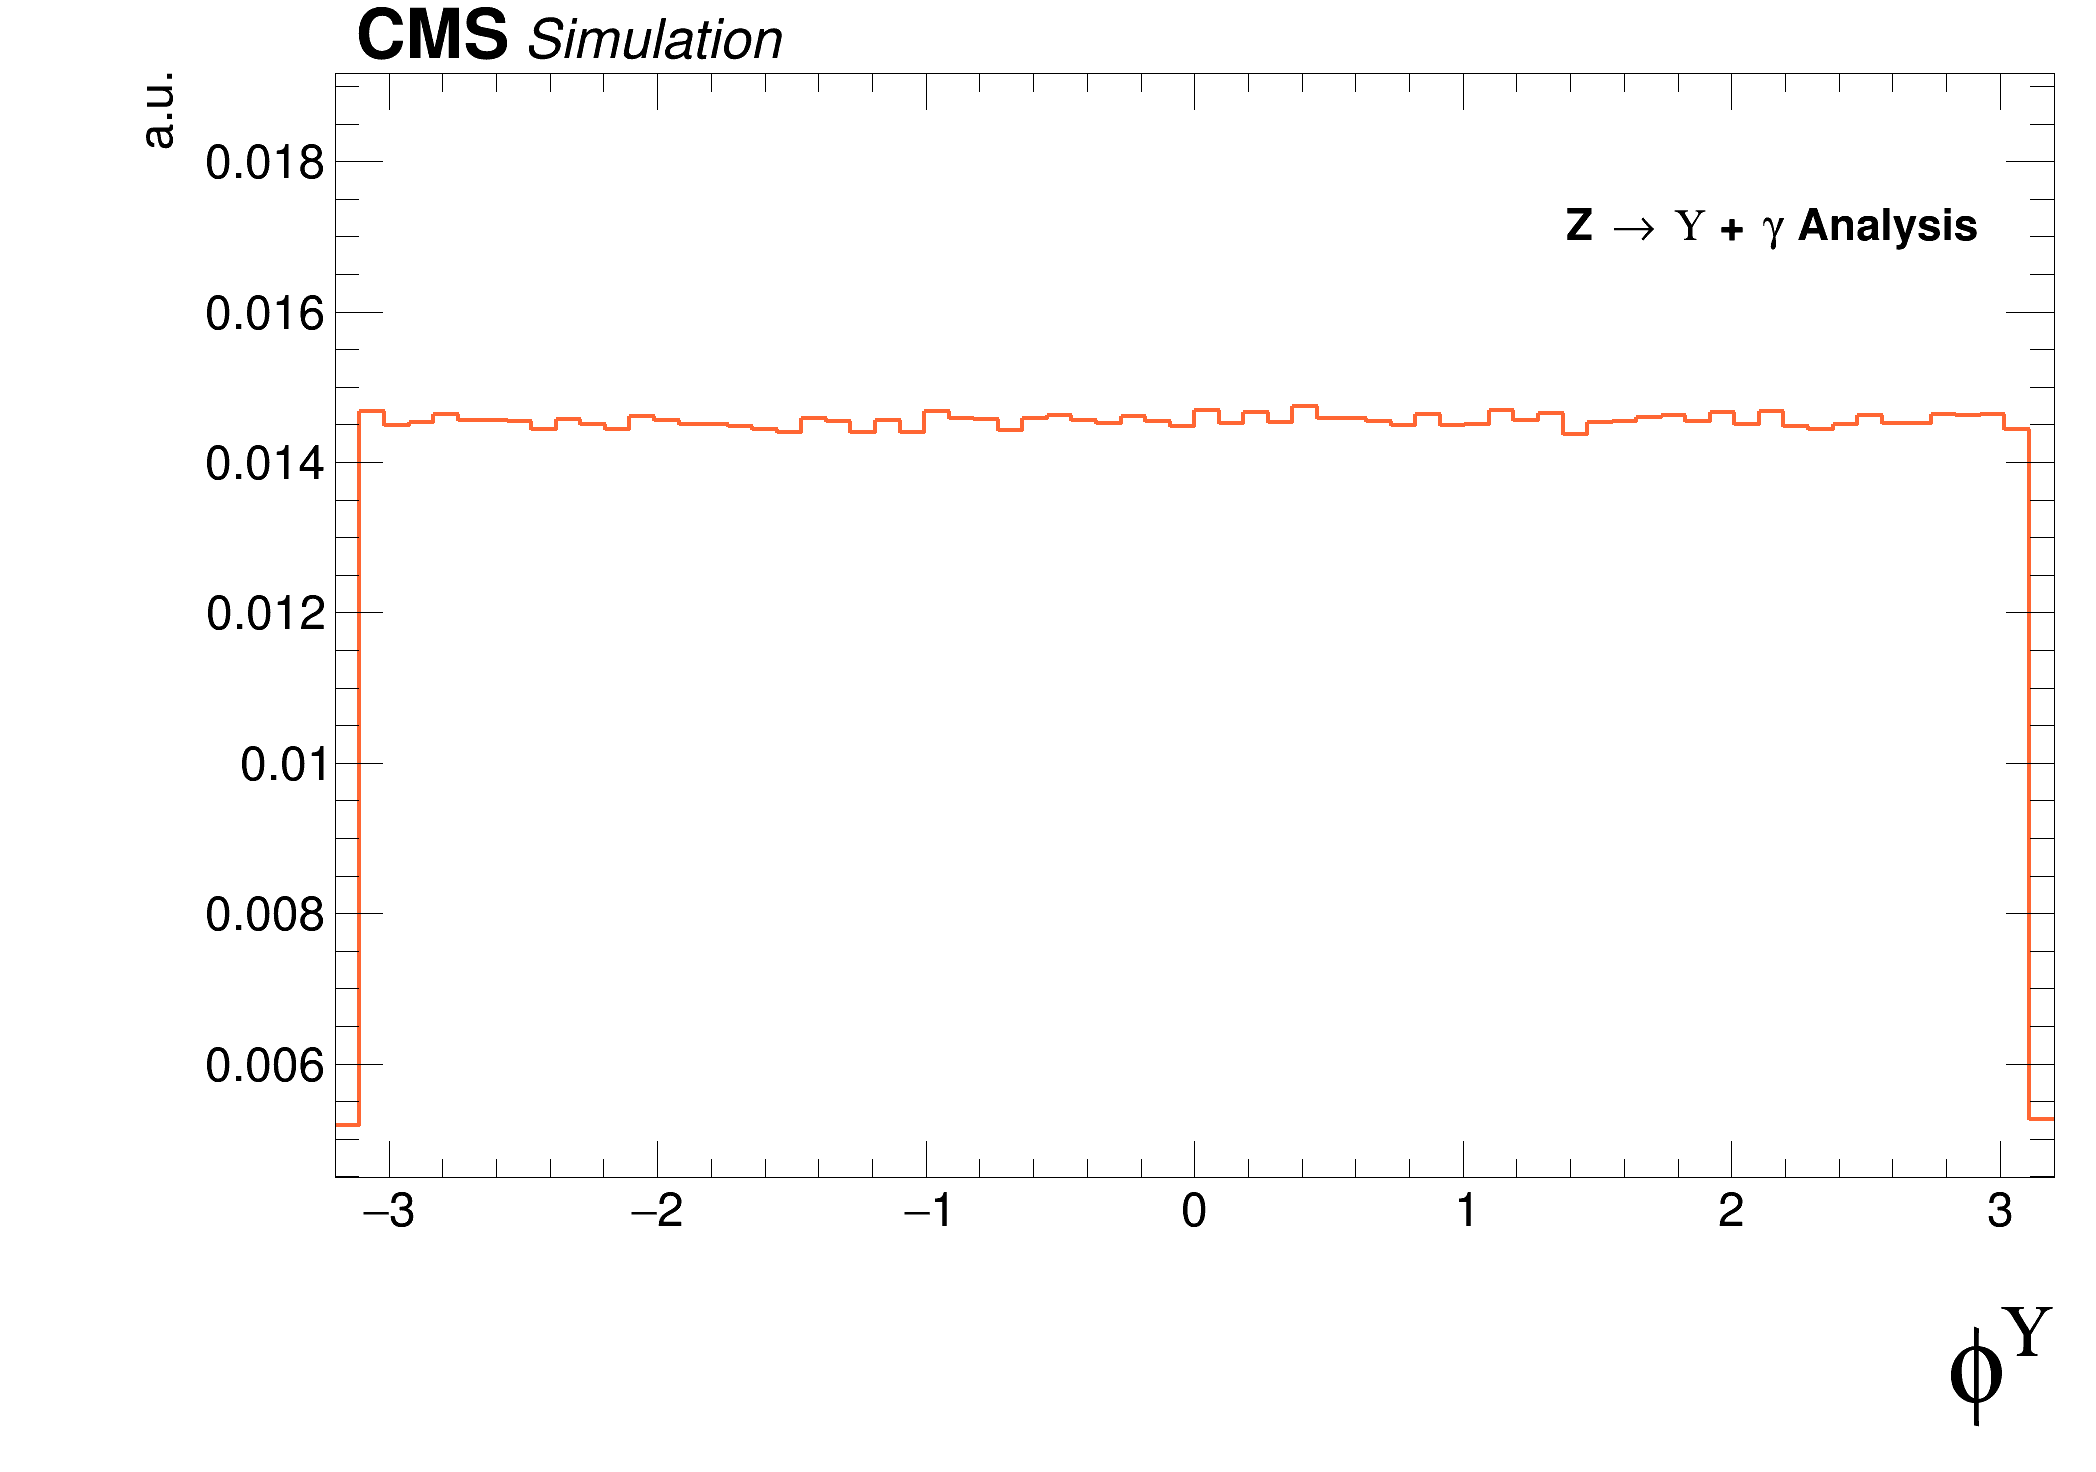
\includegraphics[width=0.25\textwidth]{figures_and_tables/outputPlots/ZtoUpsilon_Cat0_ZZZZZ/mc/unpolarized/h_Gen_Upsilon_phi}
%\hspace*{1.cm}
%Z
%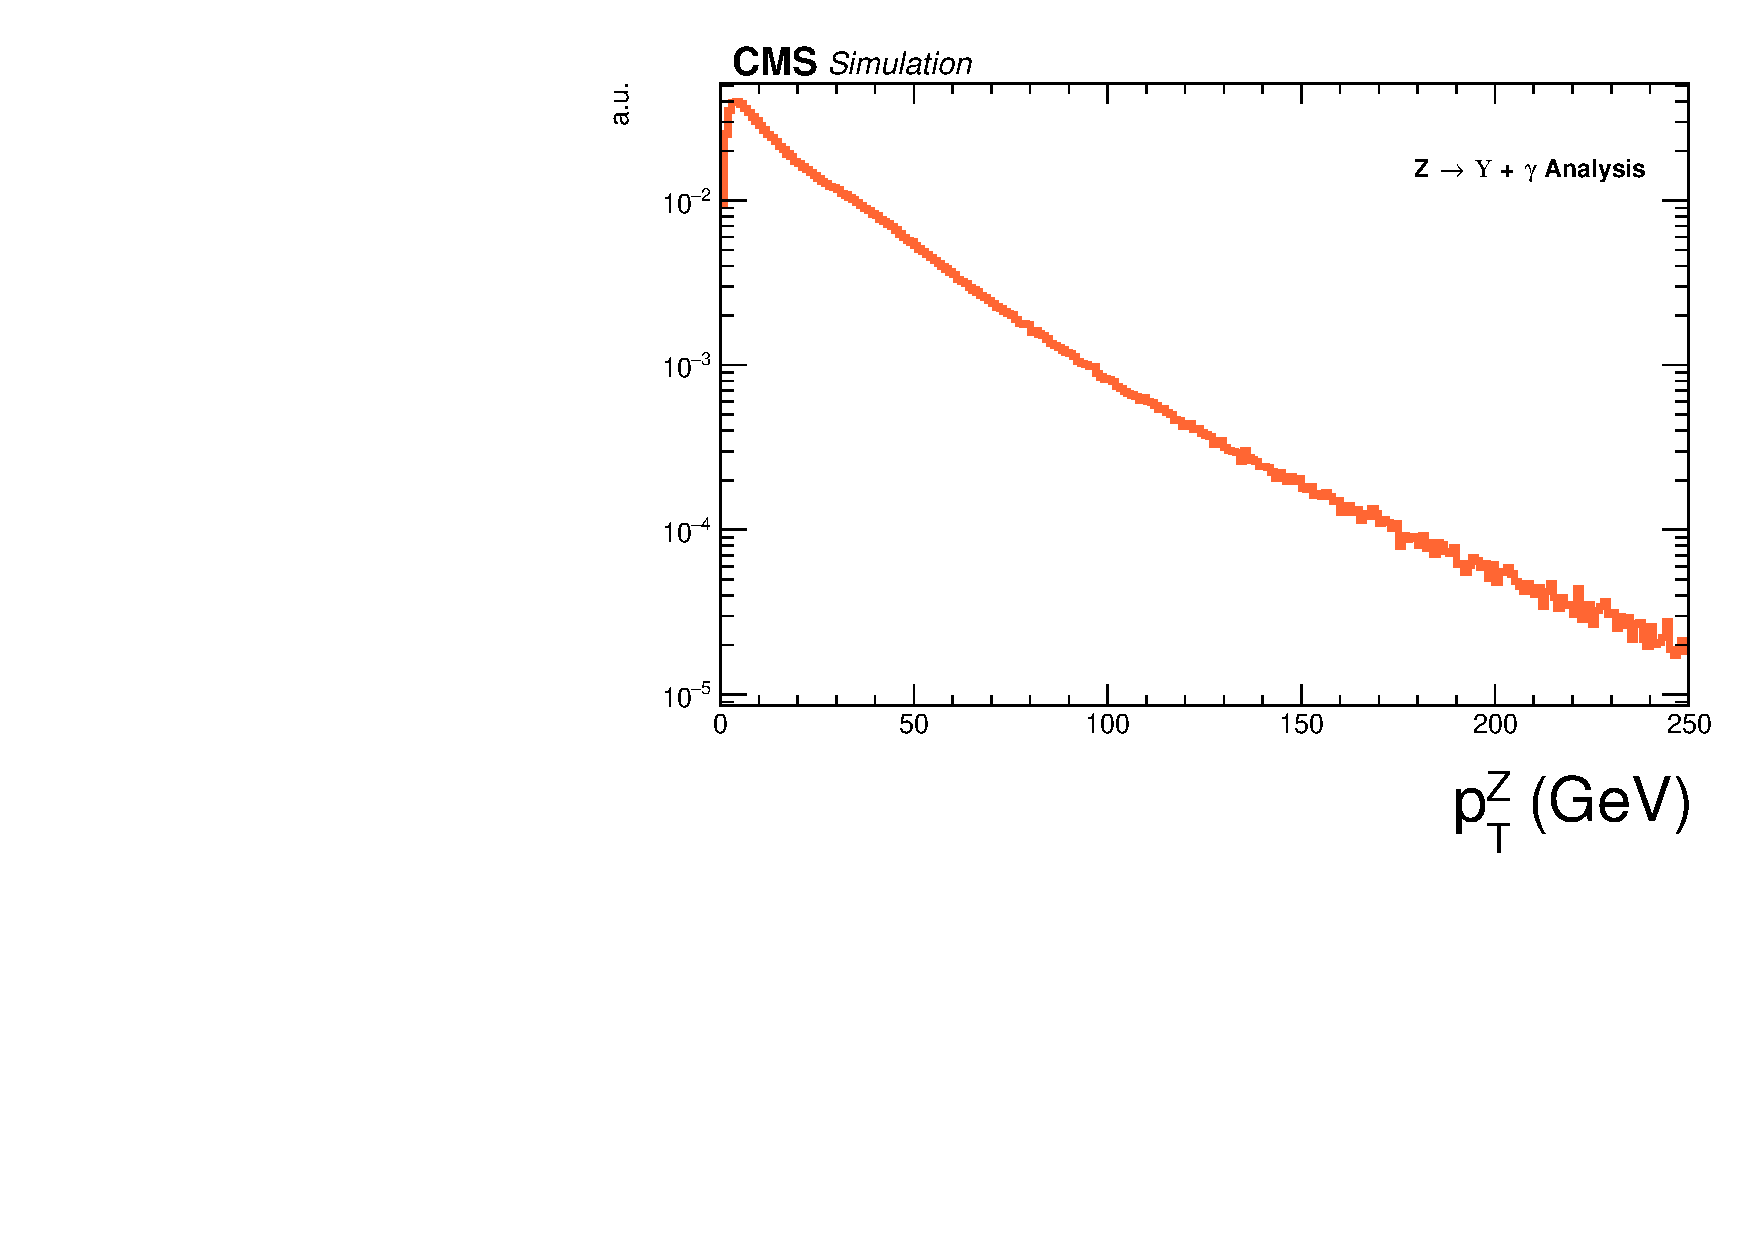
\includegraphics[width=0.25\textwidth]{figures_and_tables/outputPlots/ZtoUpsilon_Cat0_ZZZZZ/mc/unpolarized/h_Gen_Z_Pt}
%\hspace*{1.cm}
%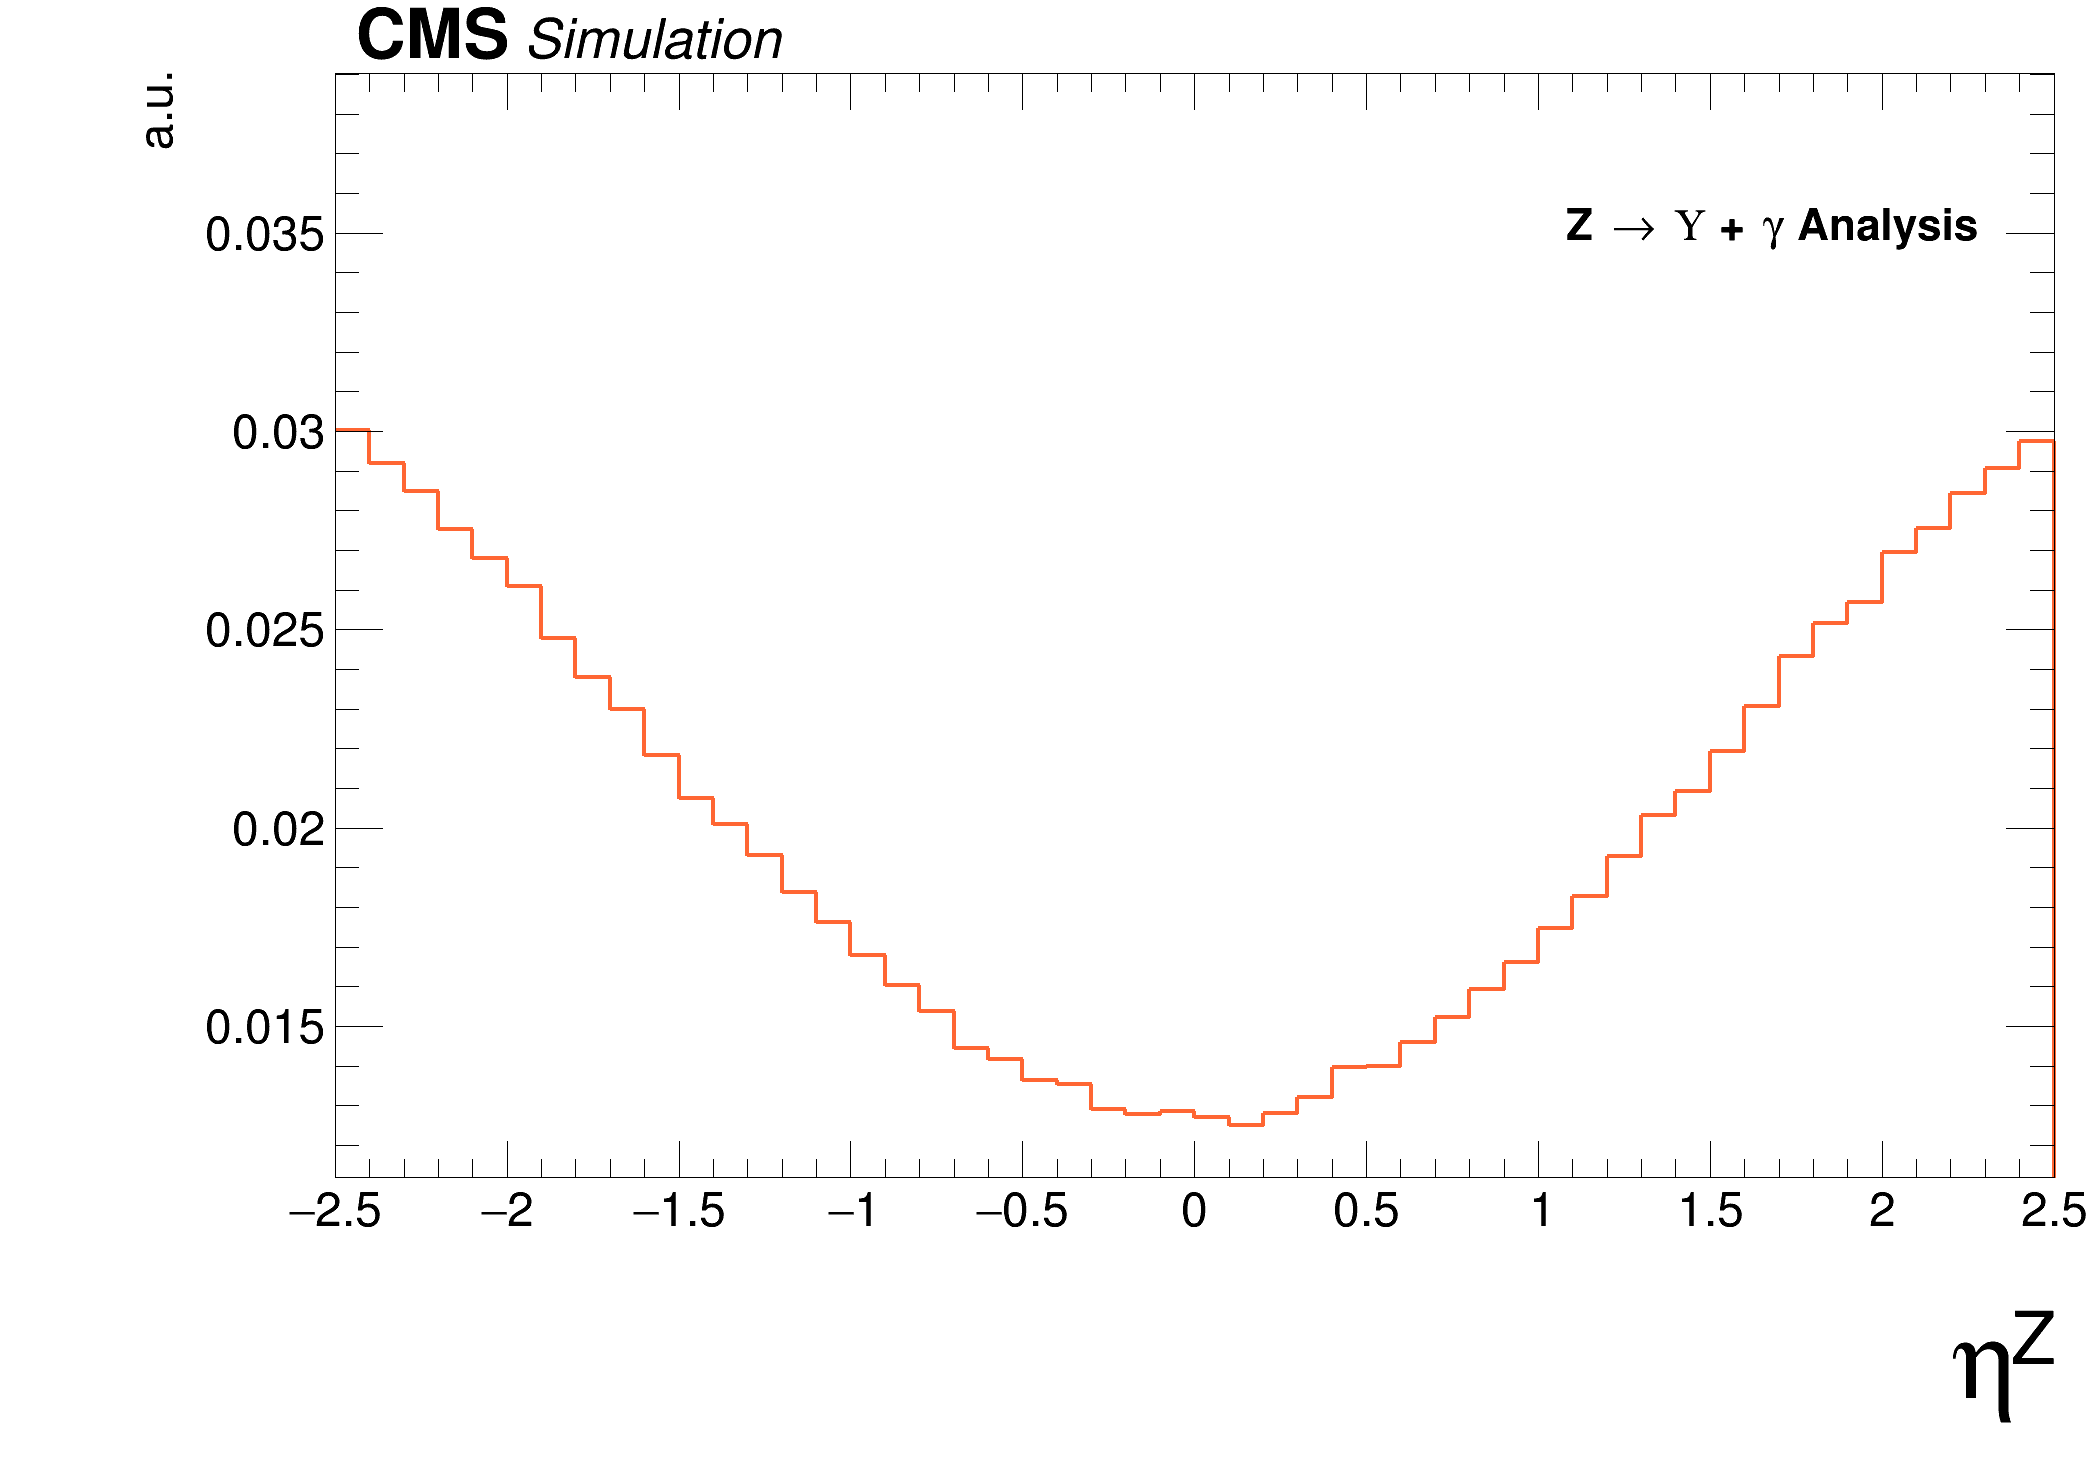
\includegraphics[width=0.25\textwidth]{figures_and_tables/outputPlots/ZtoUpsilon_Cat0_ZZZZZ/mc/unpolarized/h_Gen_Z_eta}
%\hspace*{1.cm}
%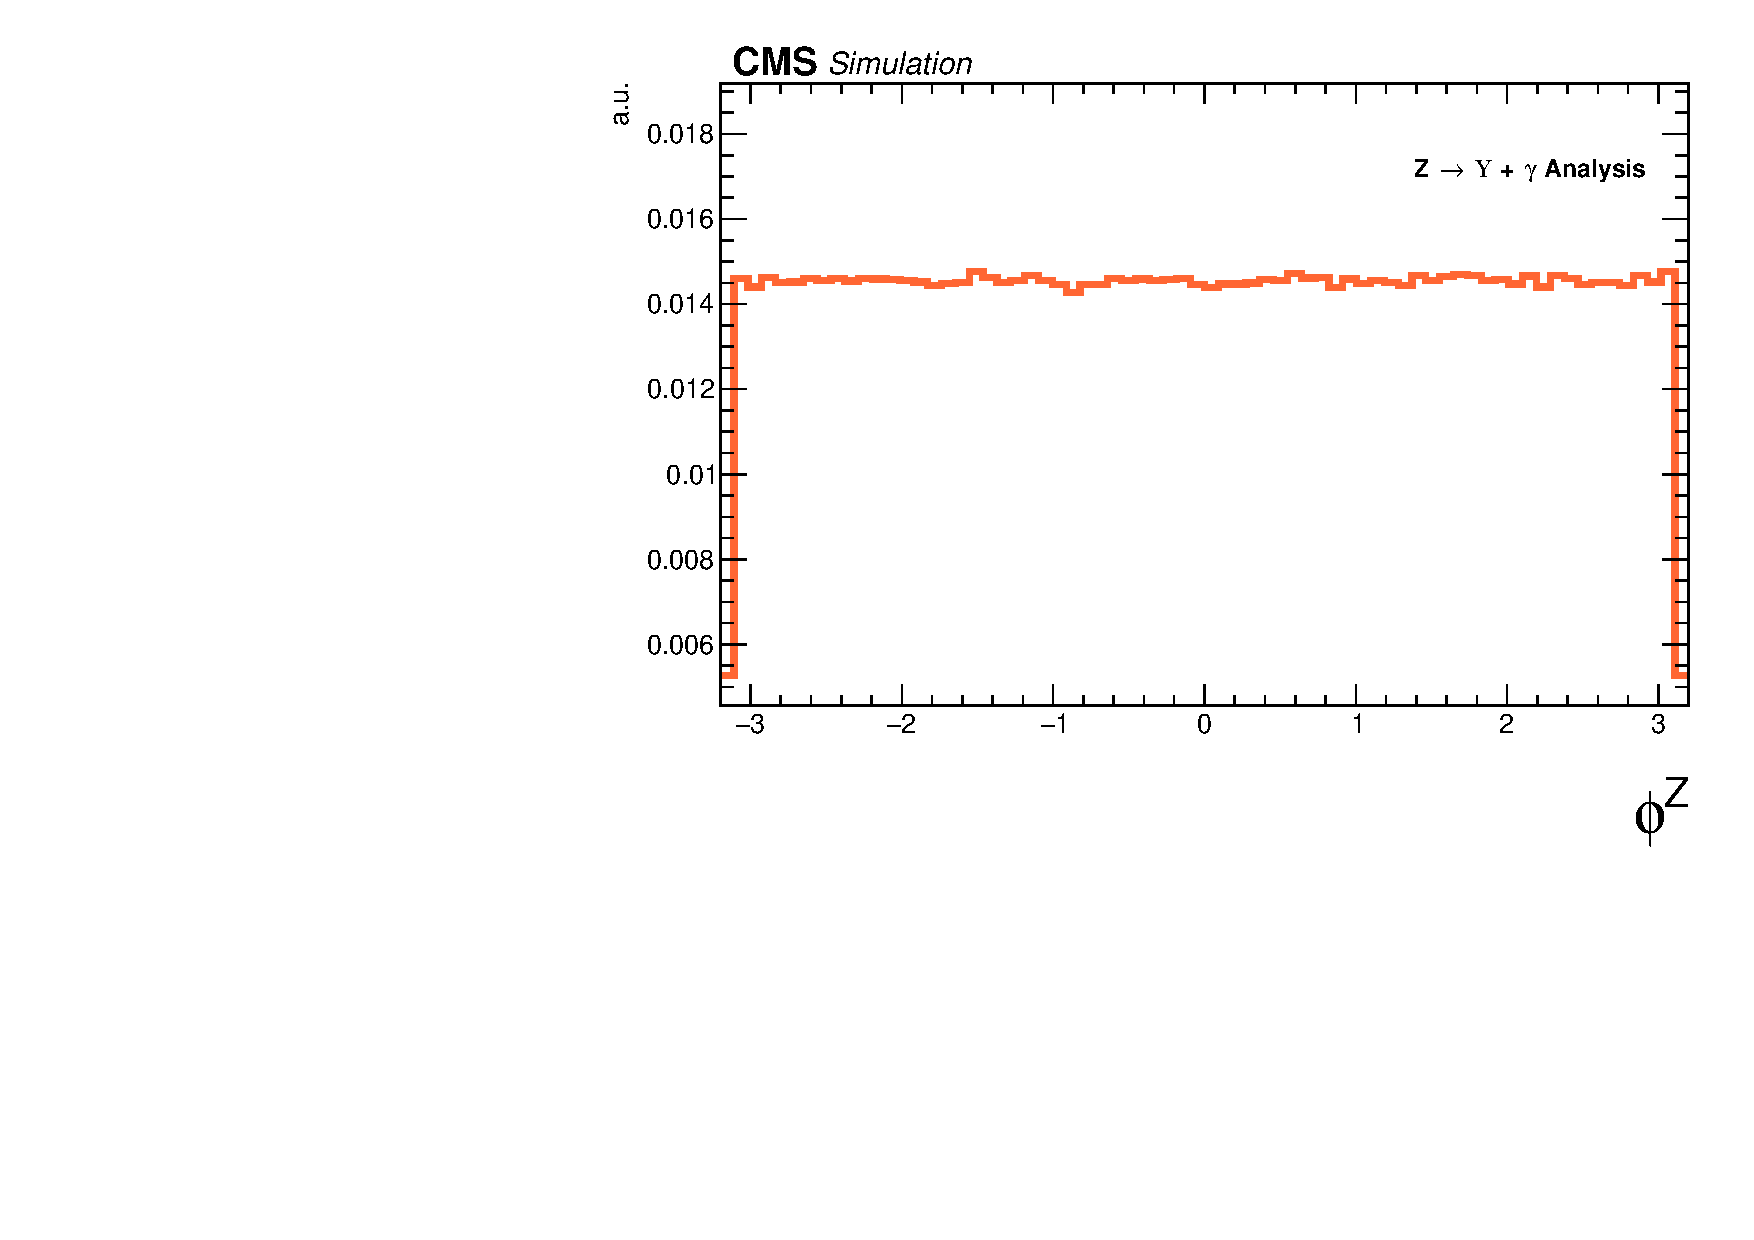
\includegraphics[width=0.25\textwidth]{figures_and_tables/outputPlots/ZtoUpsilon_Cat0_ZZZZZ/mc/unpolarized/h_Gen_Z_phi}
%\hspace*{1.cm}
%h_Gen_deltaR_Mu_Photon.png
\end{center}%\vspace*{-.5cm}
\caption{Generator level distributions of main variables for $Z\rightarrow  \Upsilon(1S,2S,3S) + \gamma$ : Transverse momenta of the leading/trailing \PT muon and the photon, pseudorapidity ($\eta$) and $\phi$ of the muons and the photon, distances $\Delta R$ between the two muons and between the muons and the photon. All the distributions shown in the figure are normalized to the unity of area.}
\label{fig:MC_ZtoUpsilon_Cat0}
\end{figure}


%%%%
\begin{figure}[!htbp]
\begin{center}
% Muon
%\hspace*{1.cm}
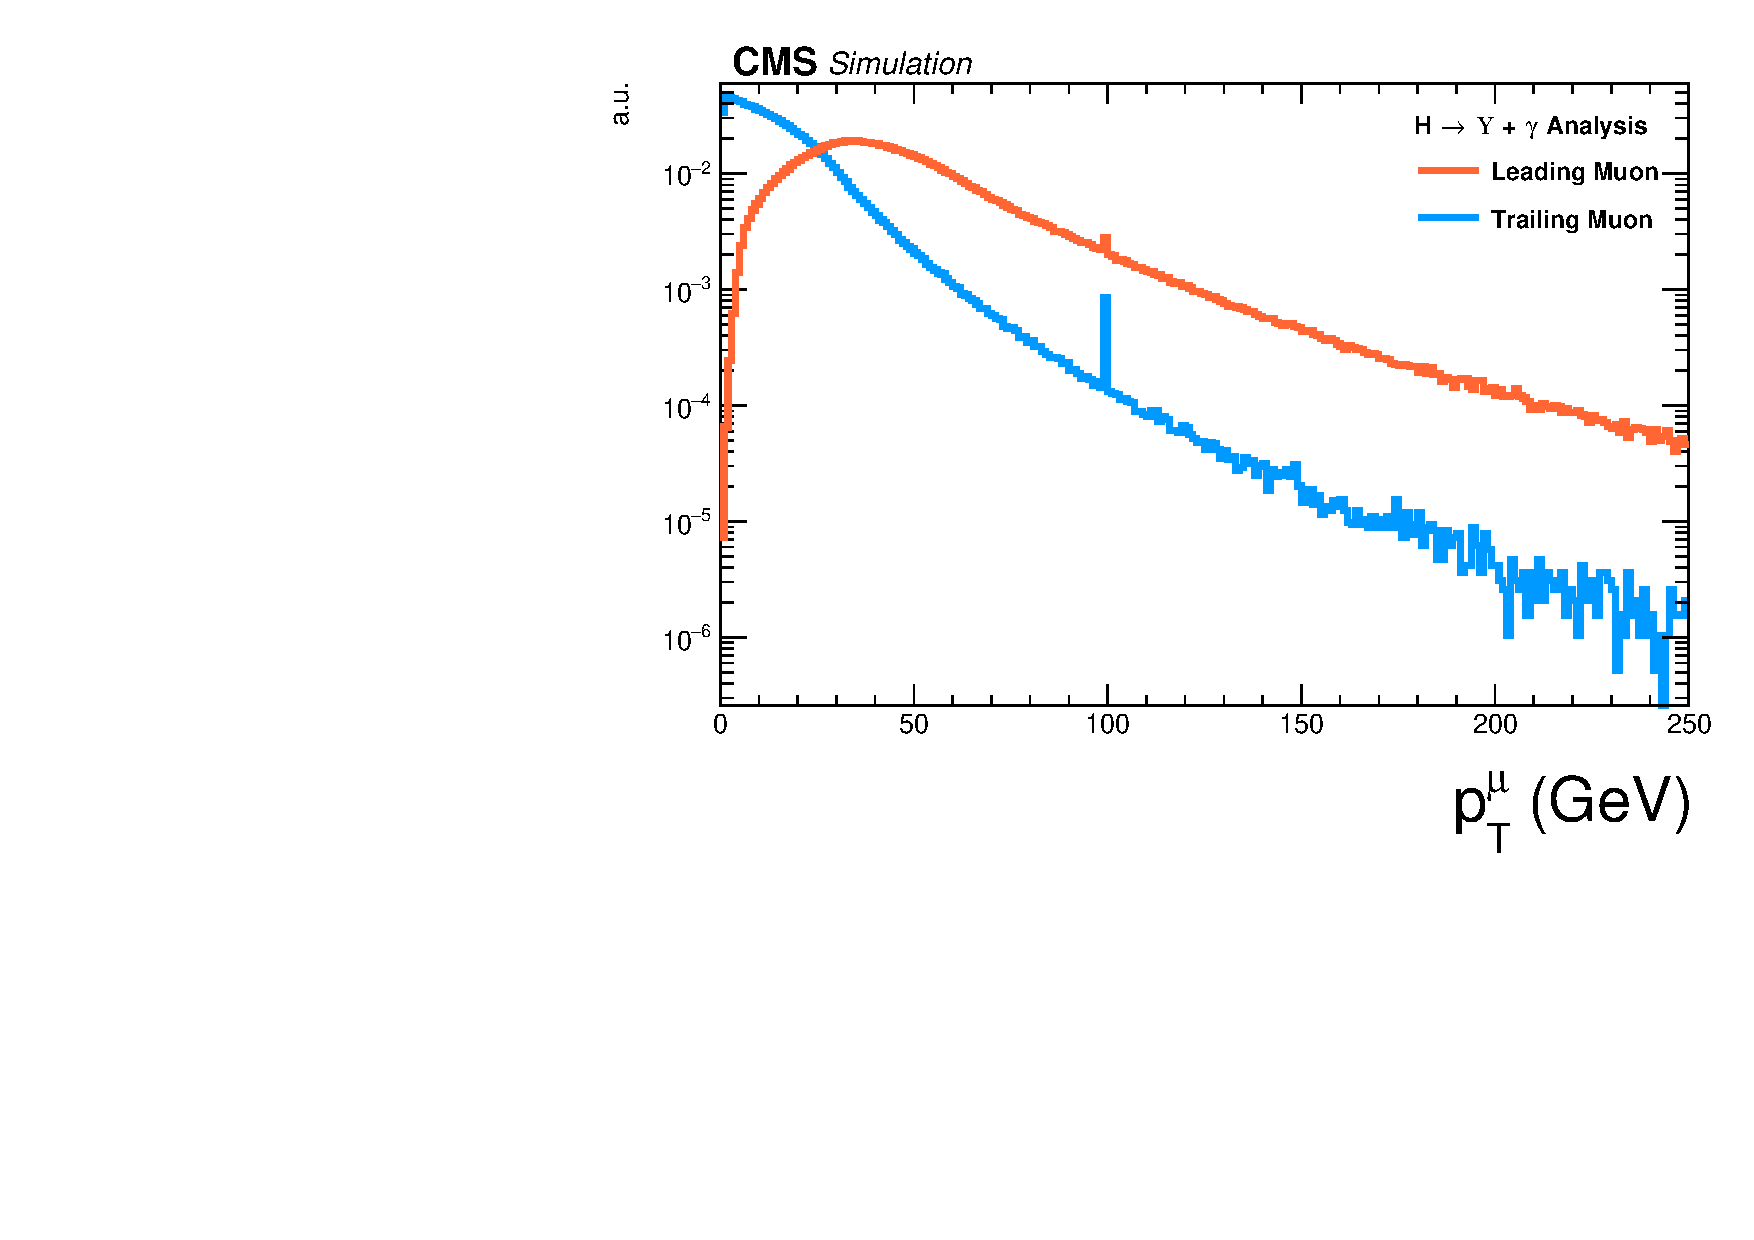
\includegraphics[width=0.45\textwidth]{figures_and_tables/outputPlots/HtoUpsilon_Cat0_ZZZZZ/mc/unpolarized/h_Gen_Mu_pt}%\hspace*{1.cm}
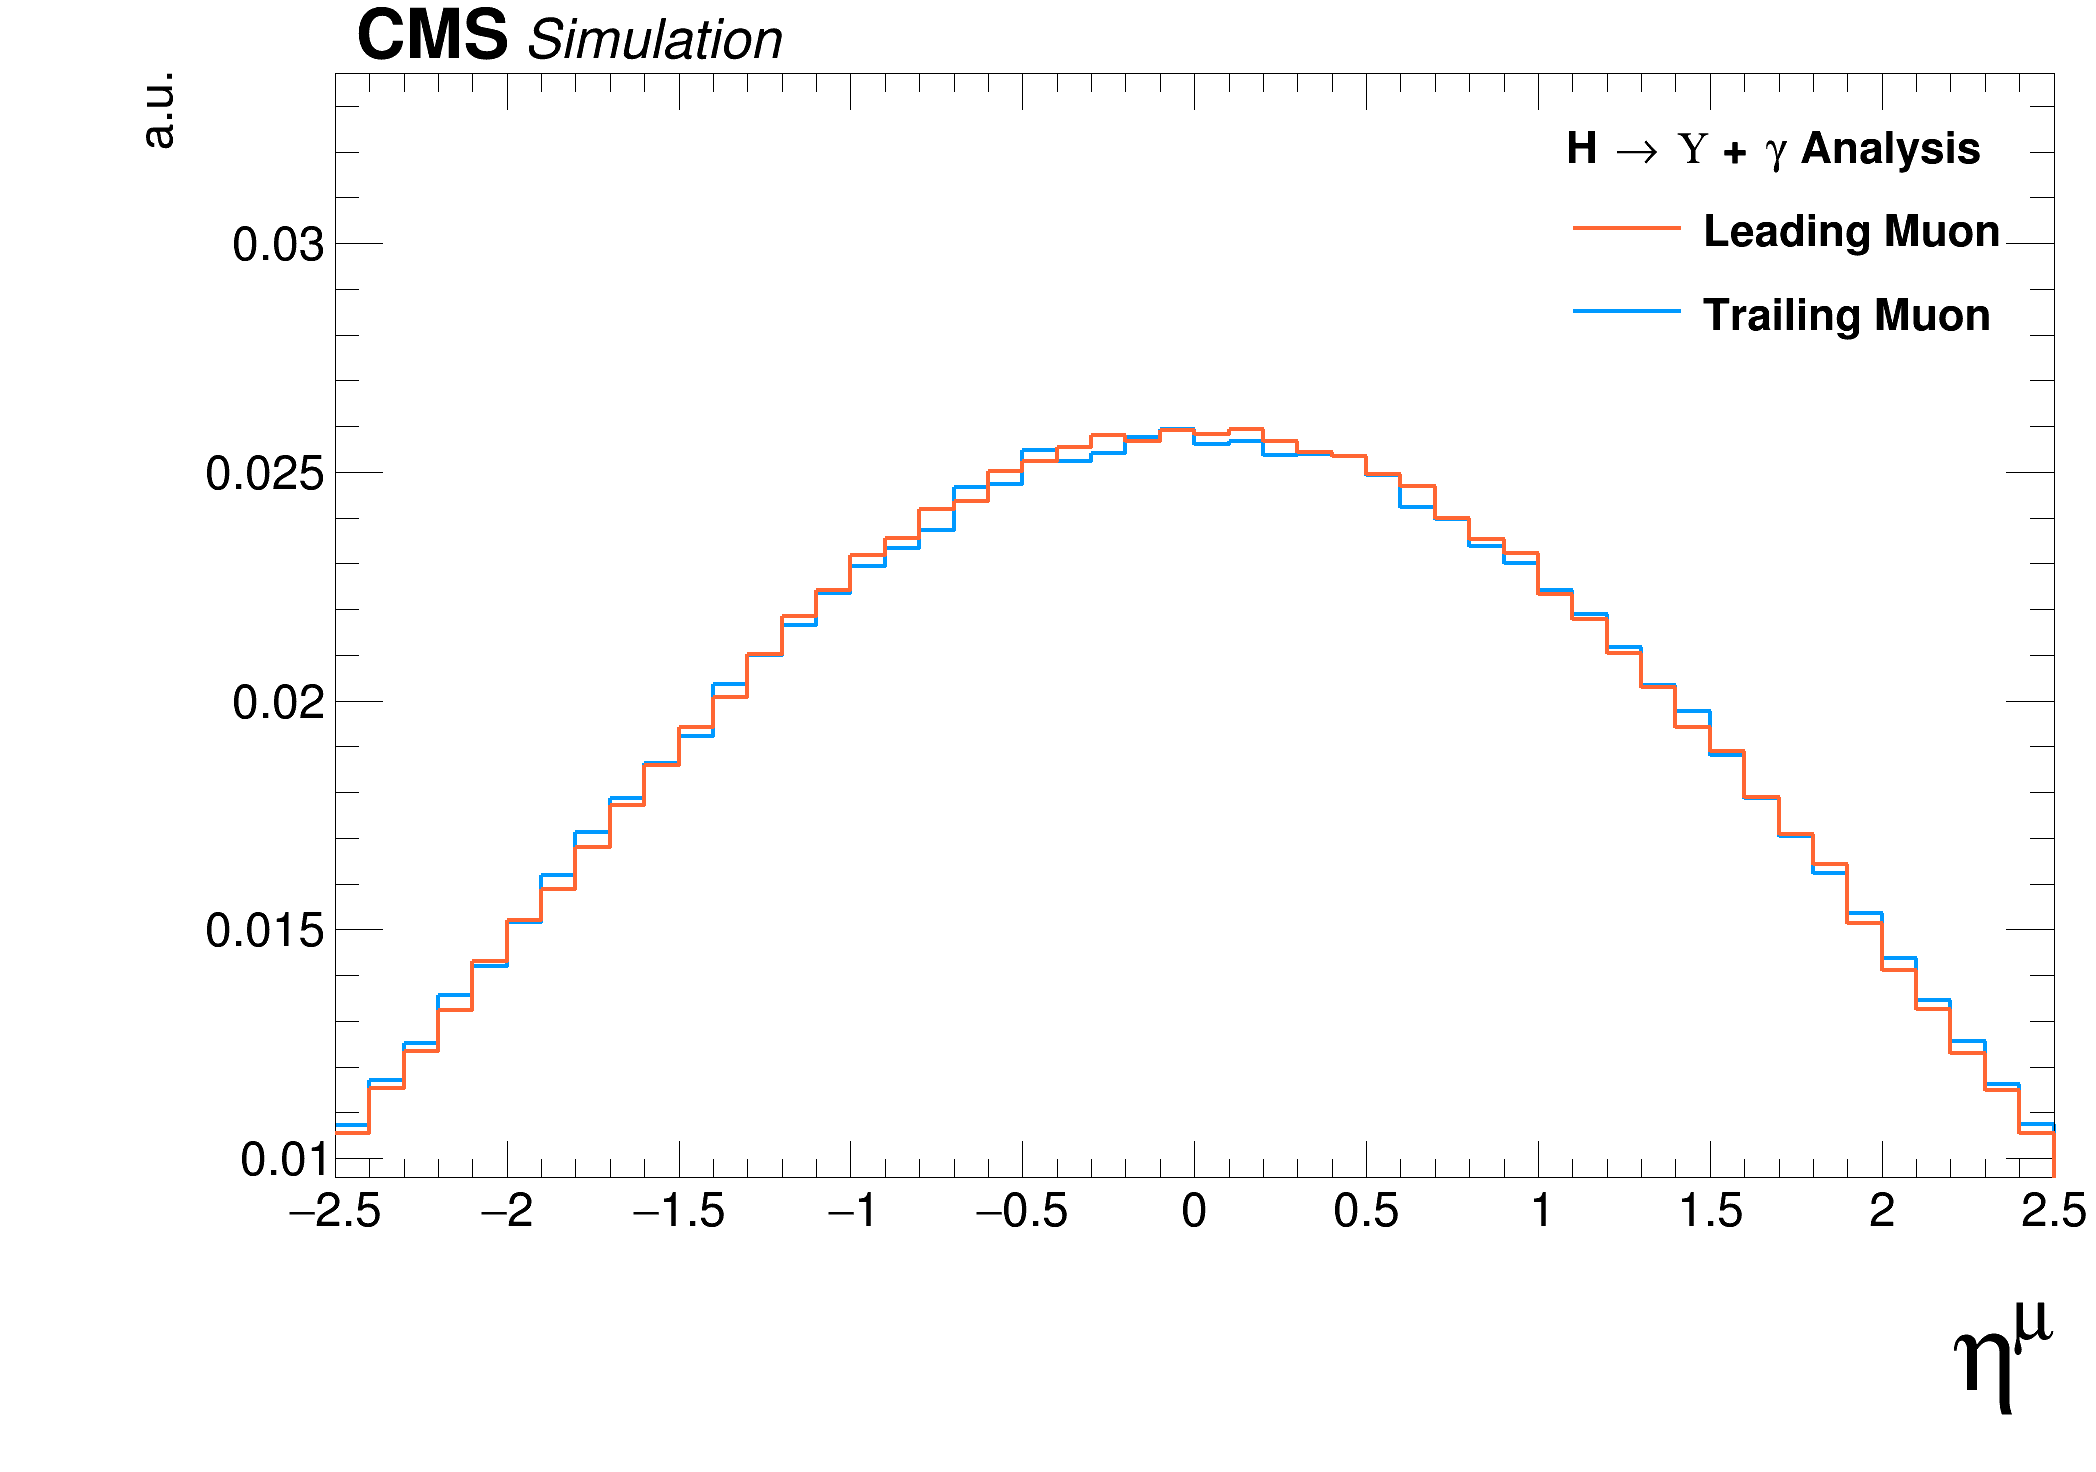
\includegraphics[width=0.45\textwidth]{figures_and_tables/outputPlots/HtoUpsilon_Cat0_ZZZZZ/mc/unpolarized/h_Gen_Mu_eta}
%\hspace*{1.cm}
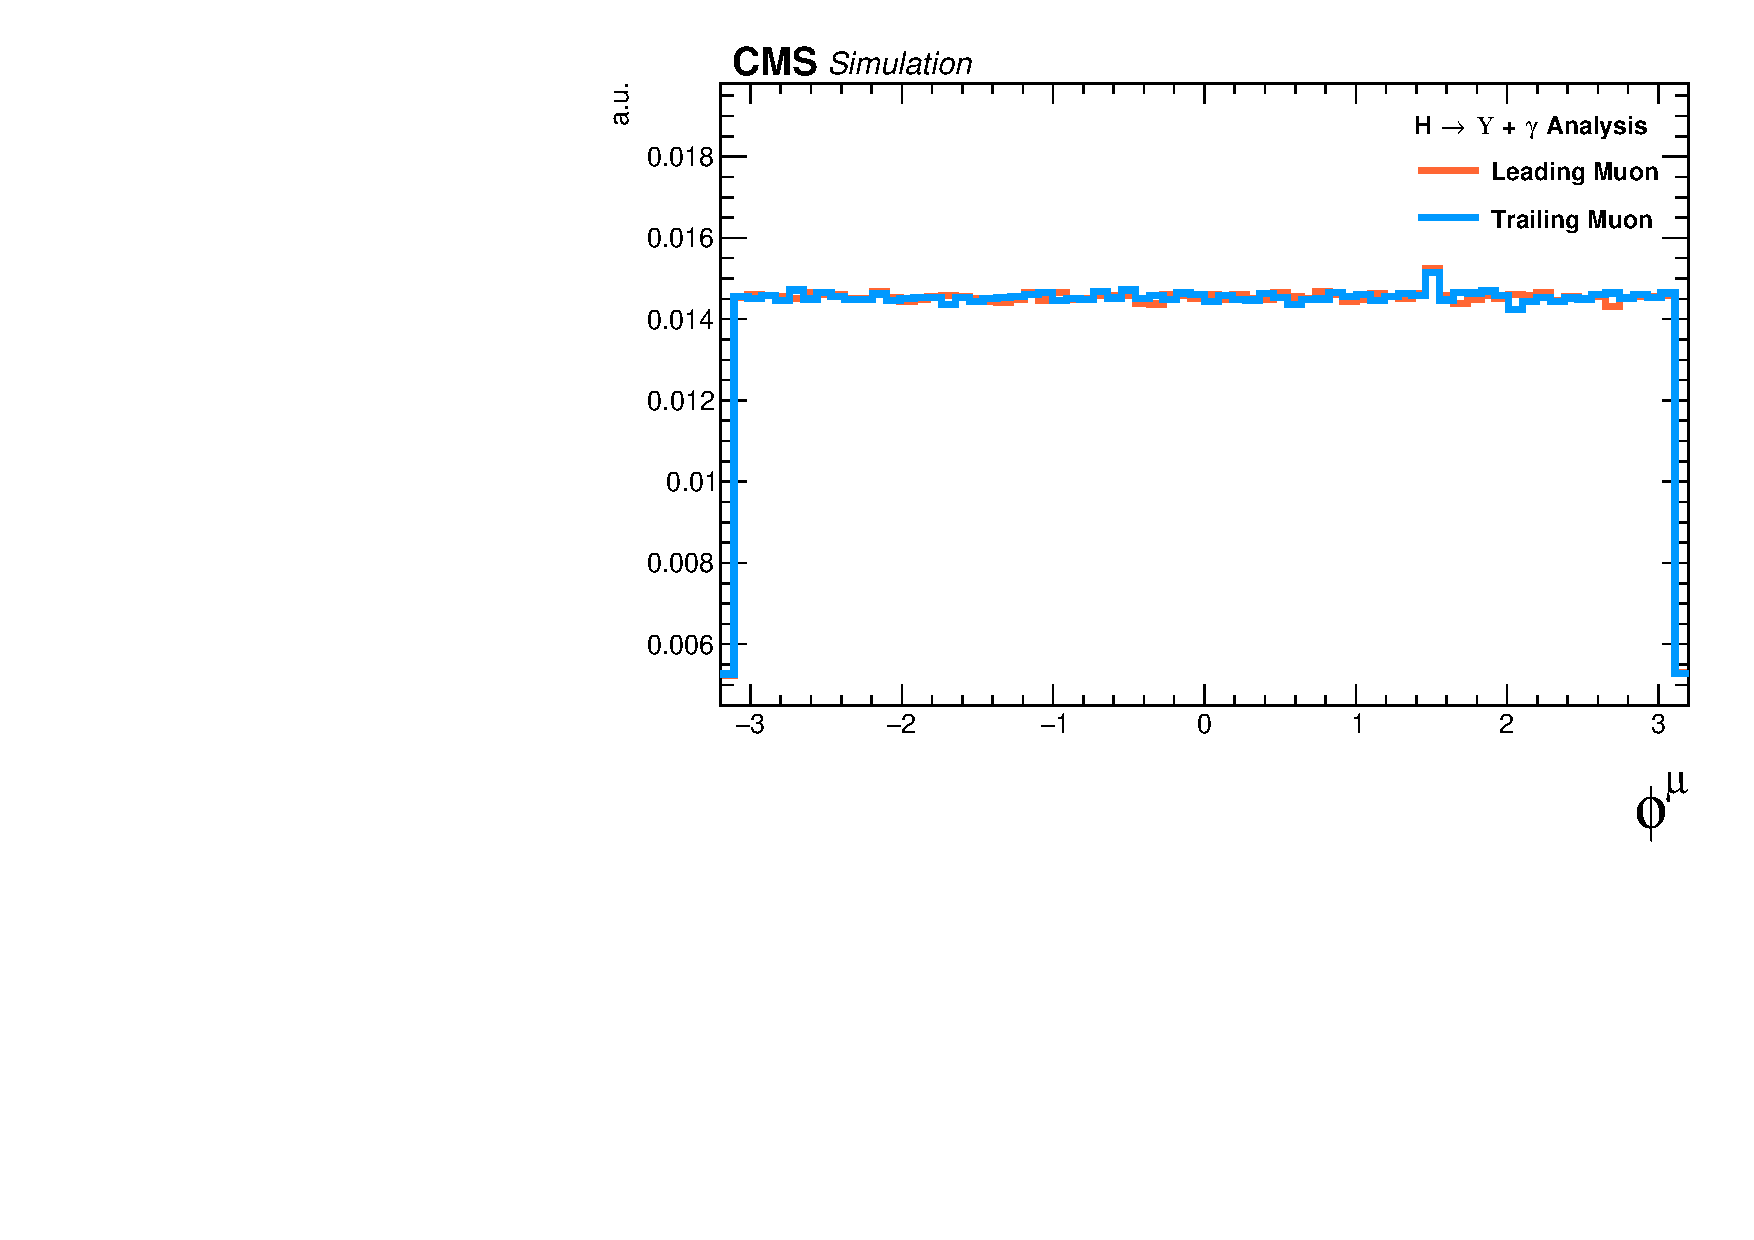
\includegraphics[width=0.45\textwidth]{figures_and_tables/outputPlots/HtoUpsilon_Cat0_ZZZZZ/mc/unpolarized/h_Gen_Mu_phi}
%\hspace*{1.cm}
%Delta R mu_trading and mu_leading
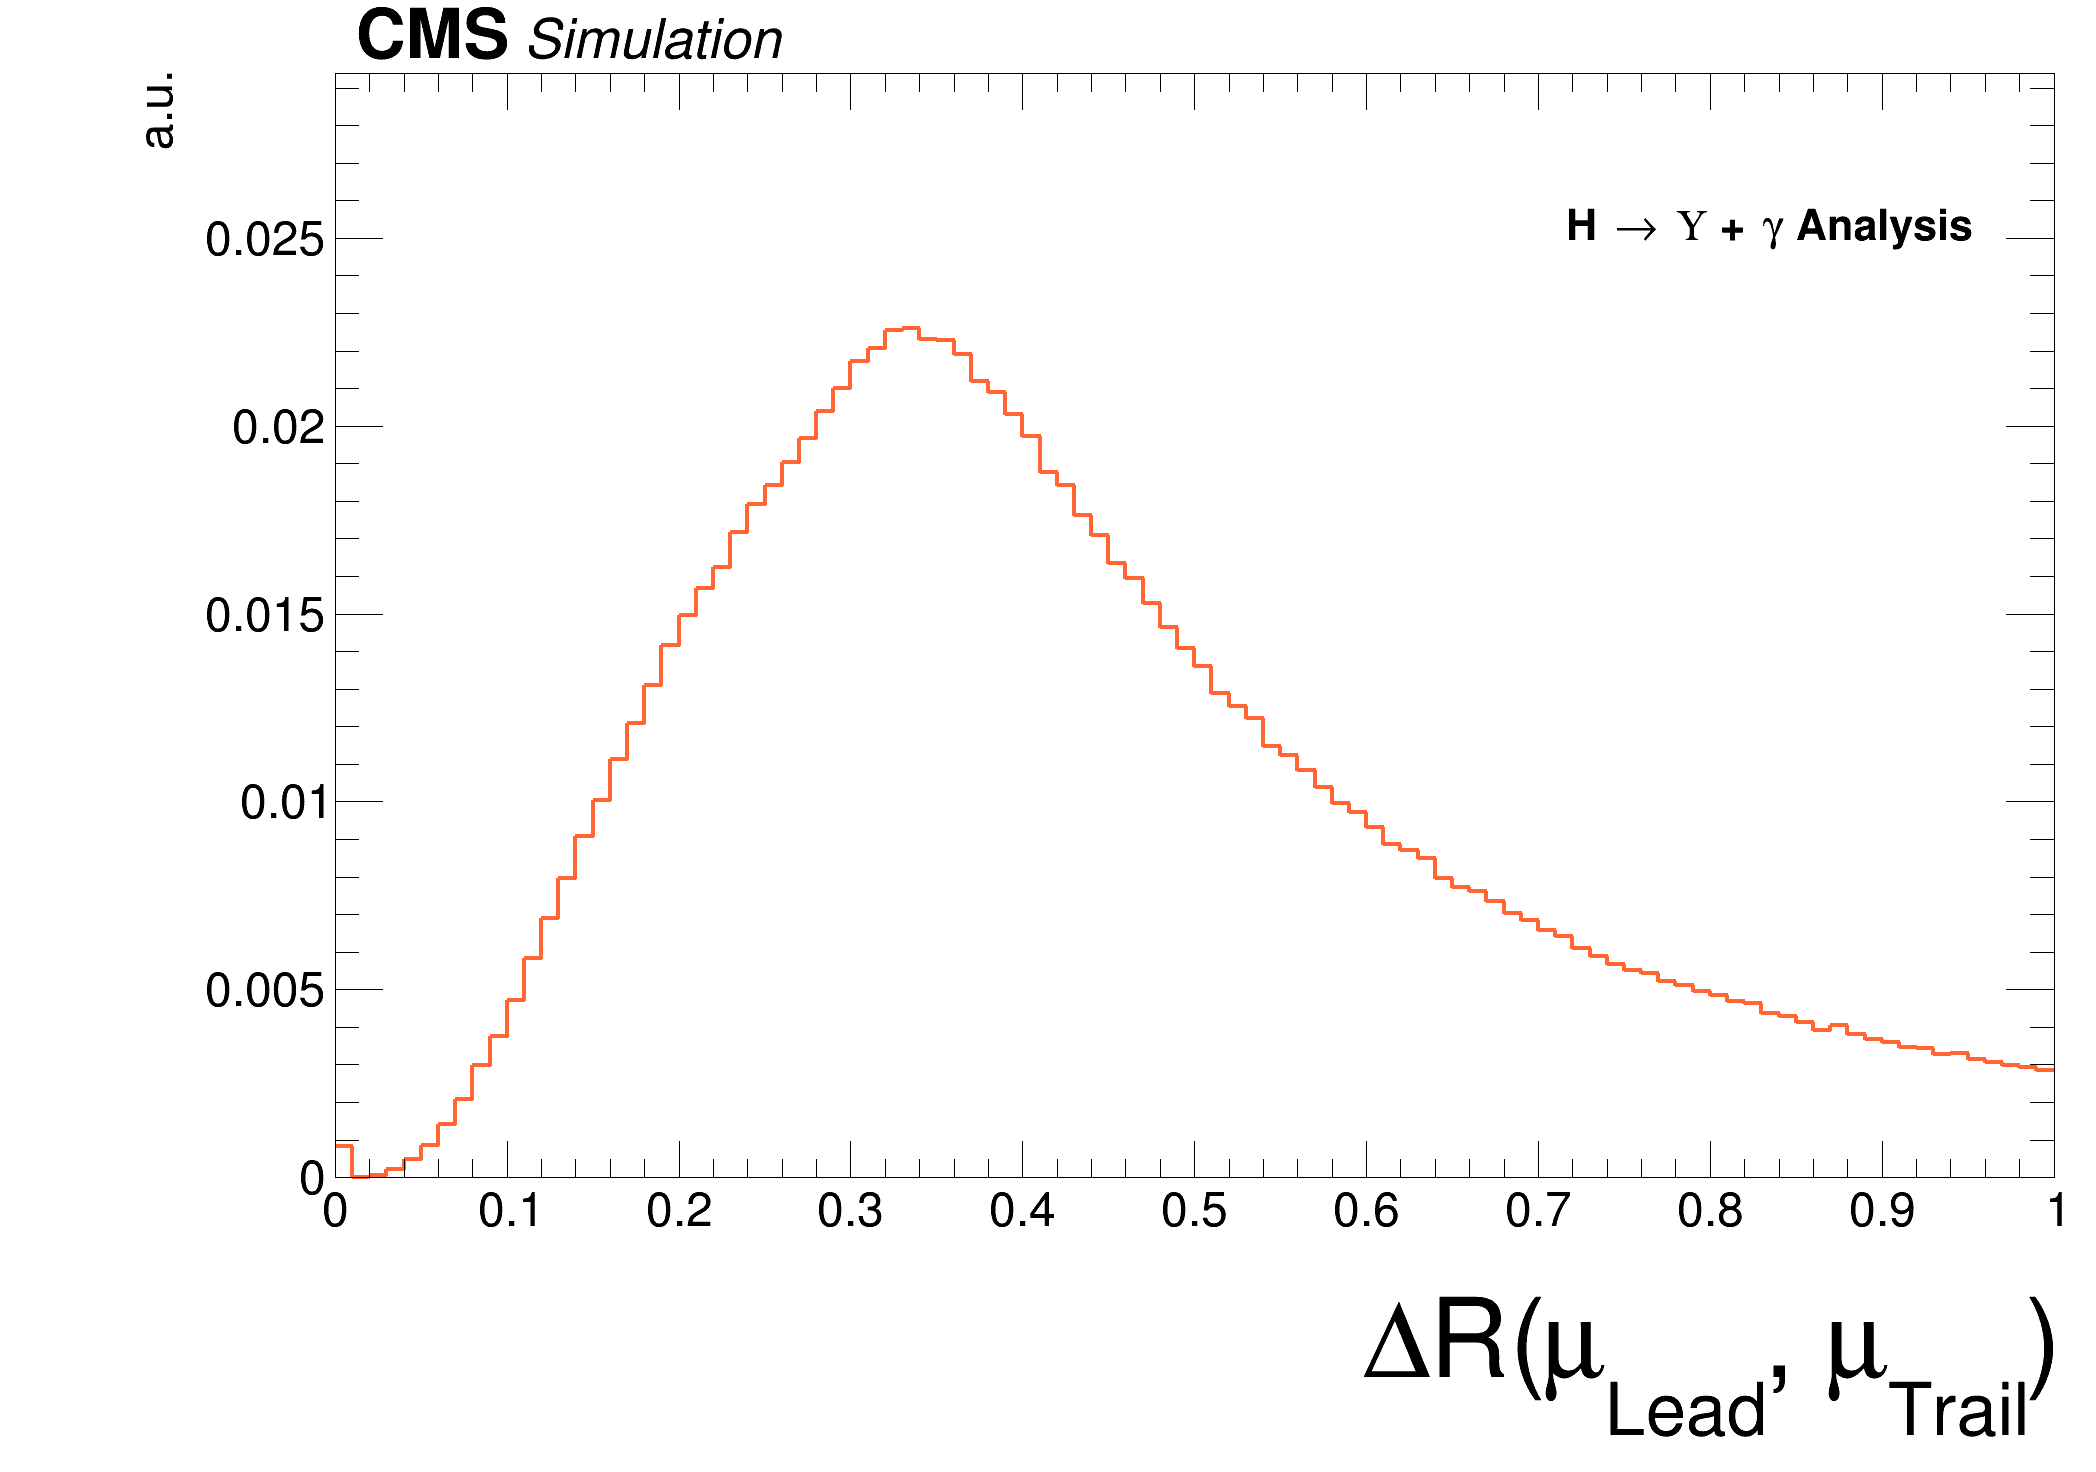
\includegraphics[width=0.45\textwidth]{figures_and_tables/outputPlots/HtoUpsilon_Cat0_ZZZZZ/mc/unpolarized/h_Gen_deltaR_Leading_Trailing}
%Photon
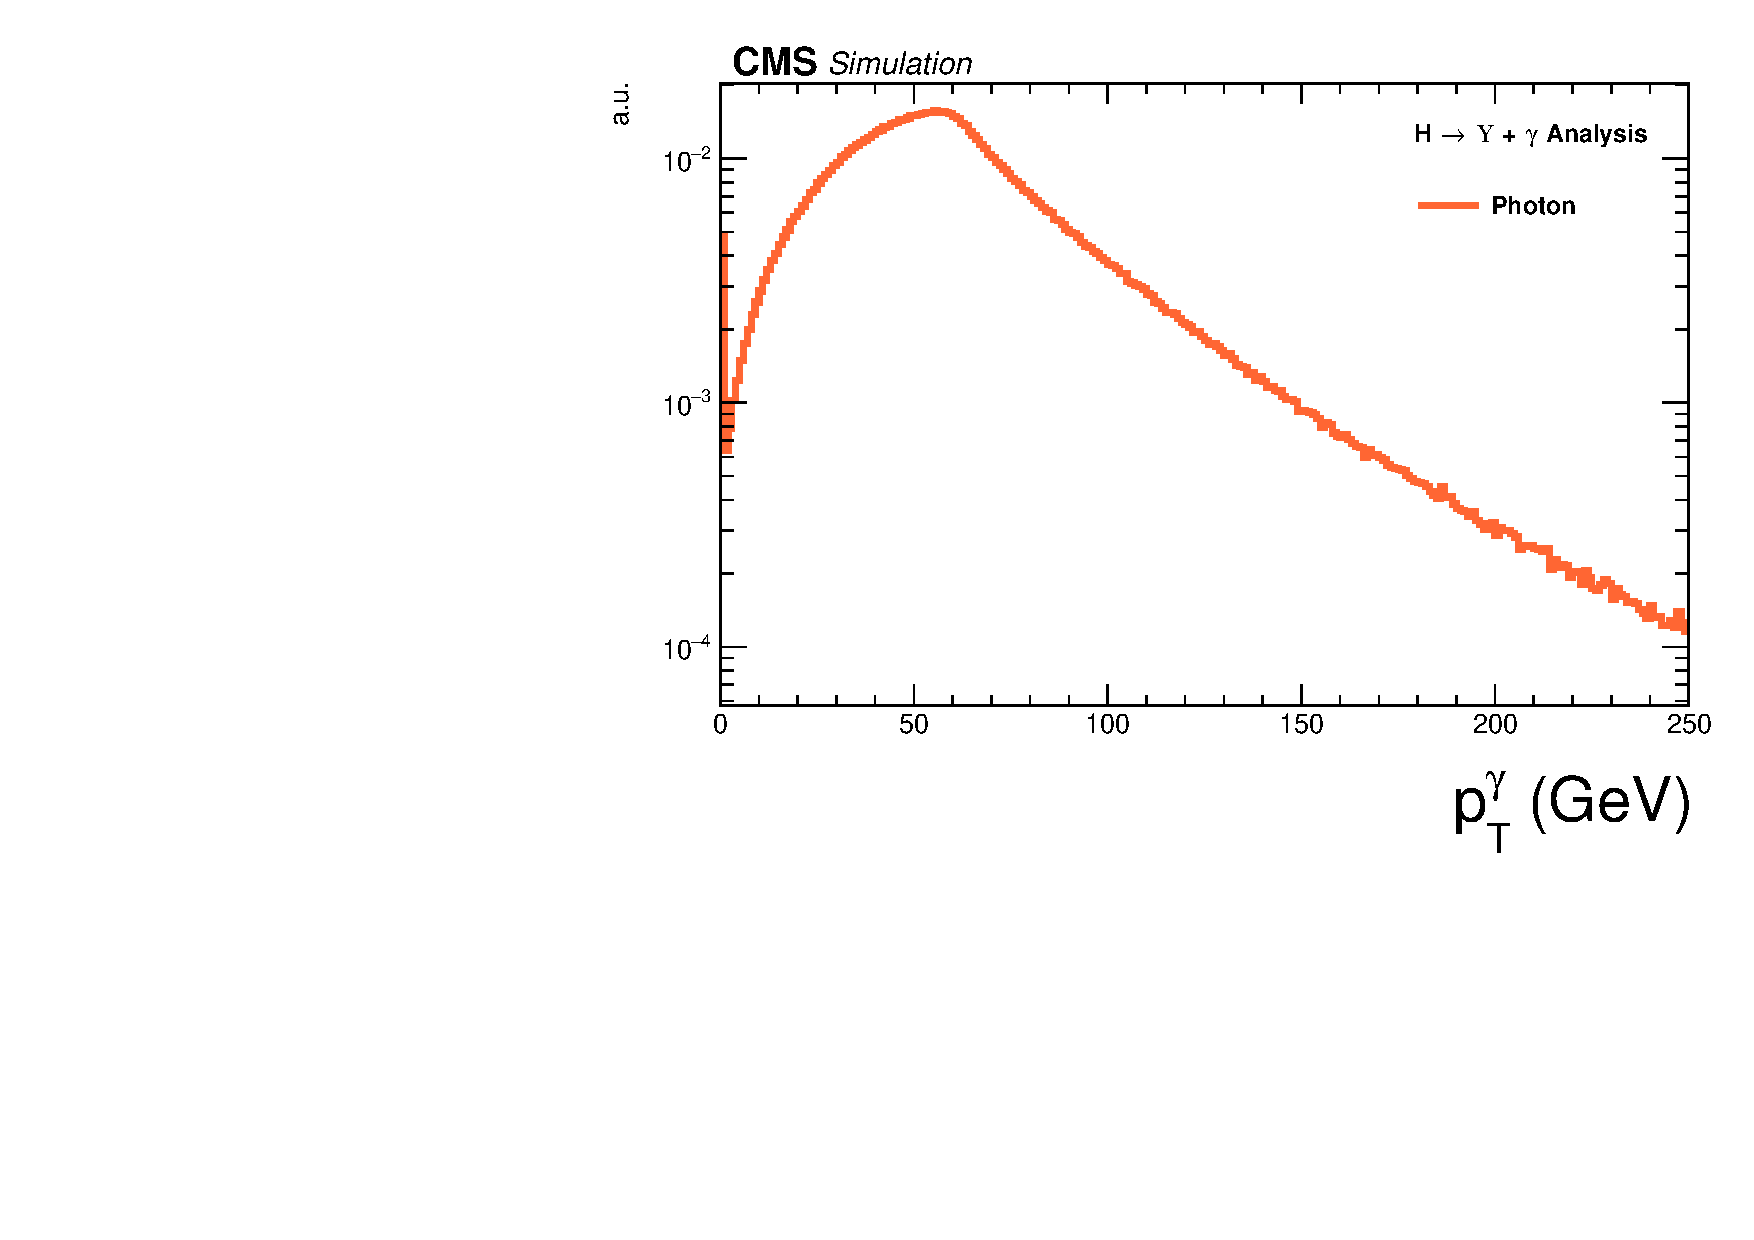
\includegraphics[width=0.45\textwidth]{figures_and_tables/outputPlots/HtoUpsilon_Cat0_ZZZZZ/mc/unpolarized/h_Gen_Photon_pt}
%\hspace*{1.cm}
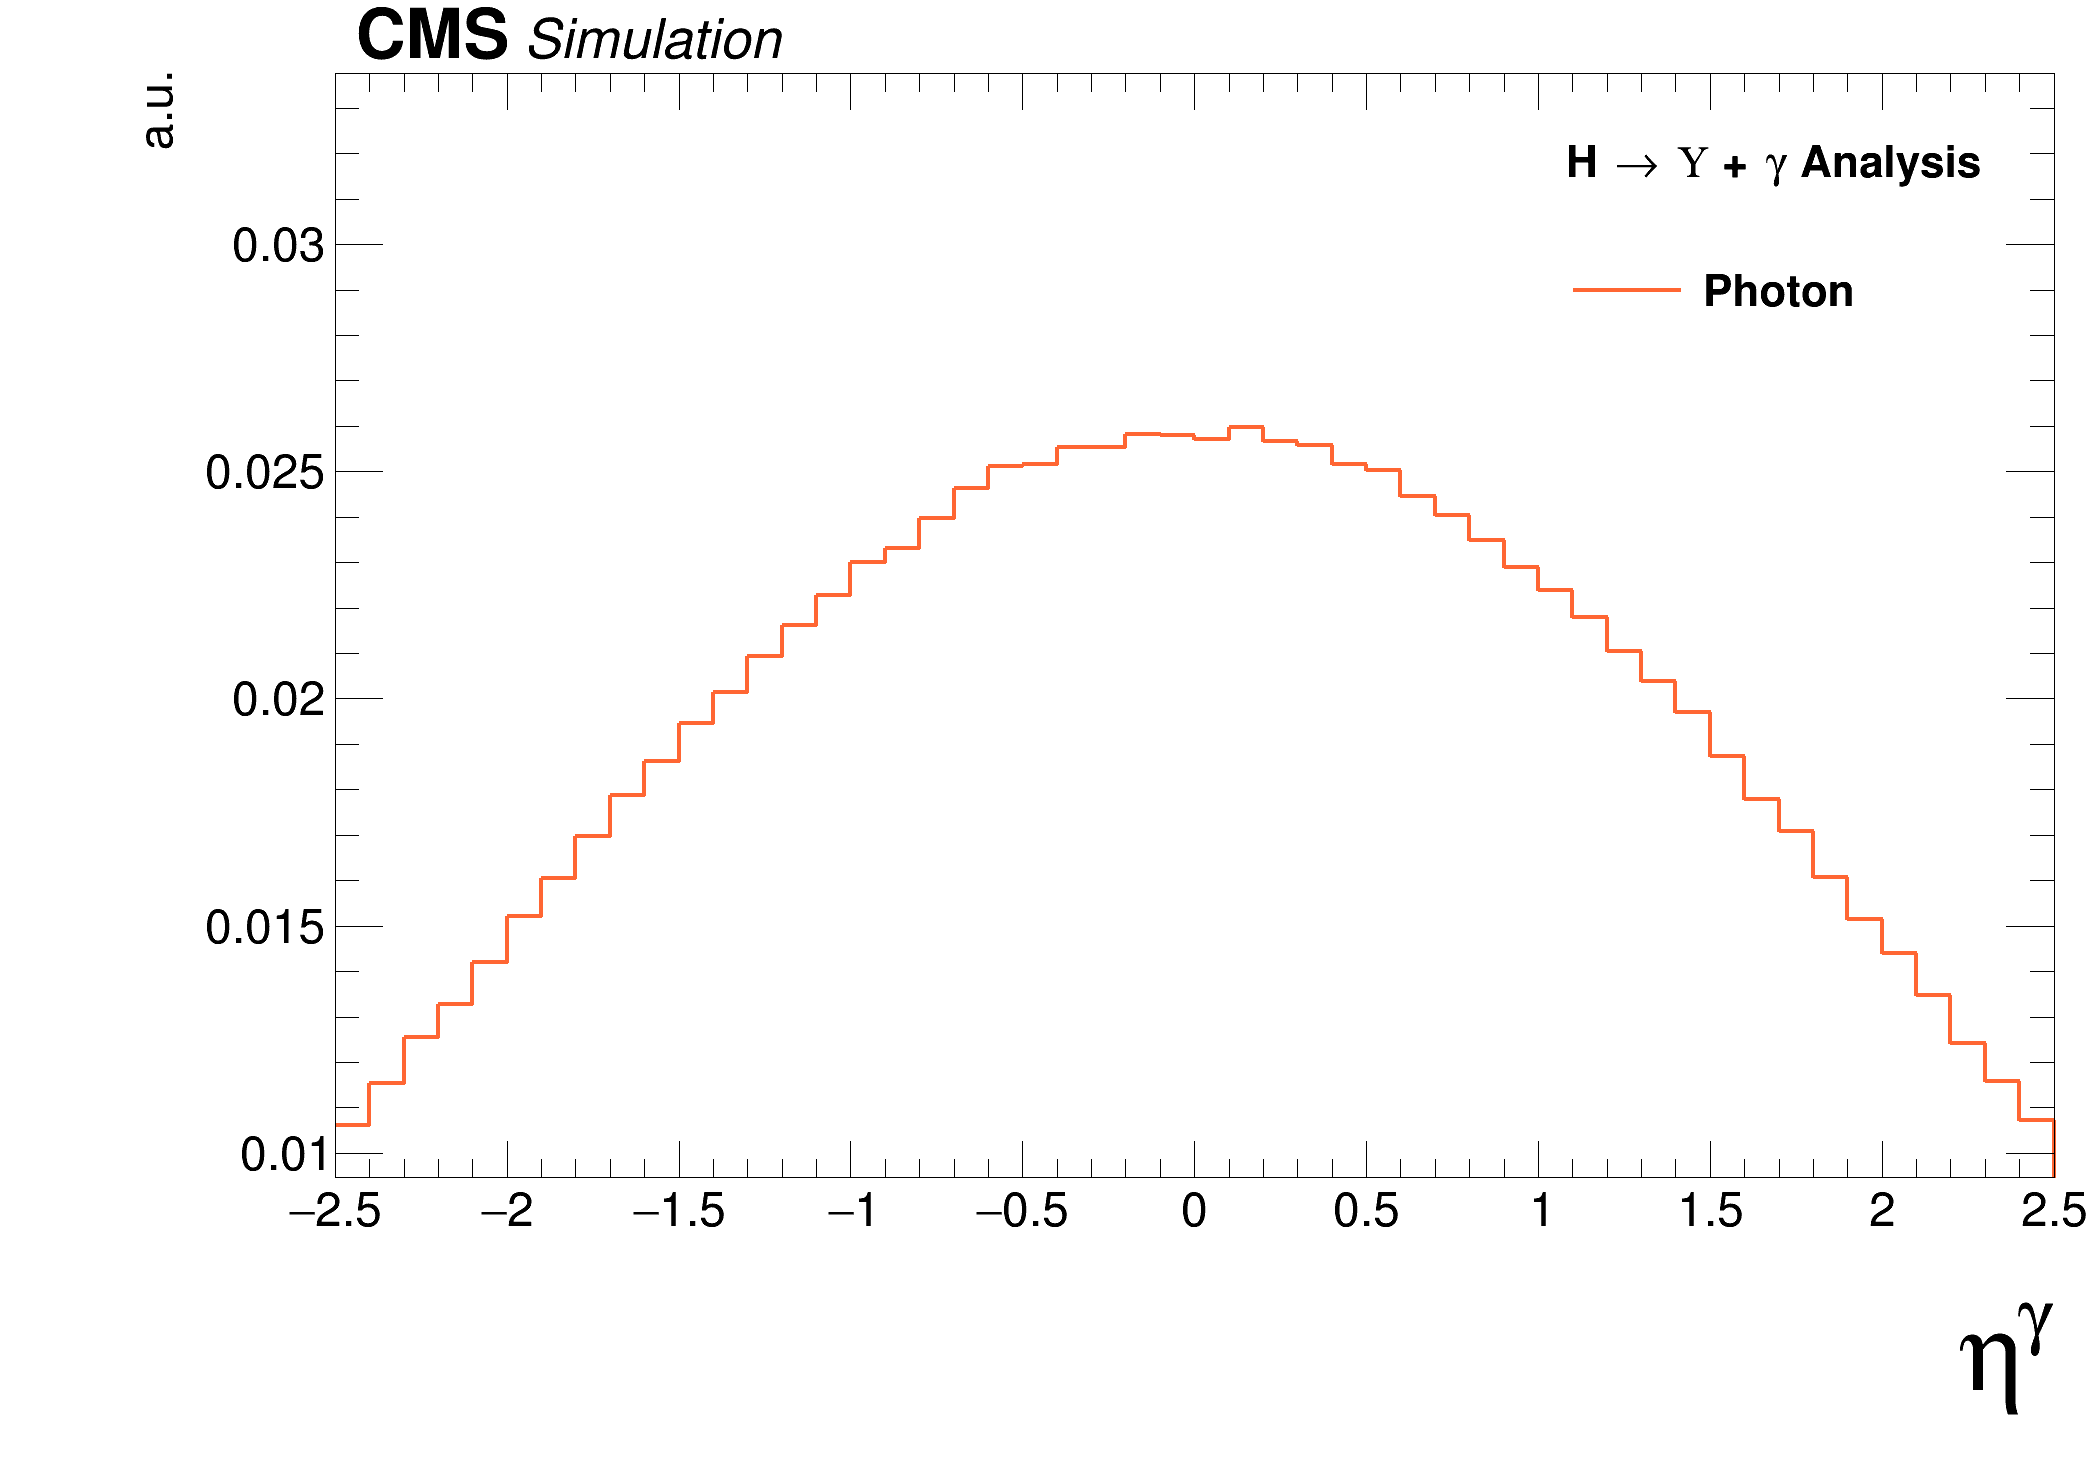
\includegraphics[width=0.45\textwidth]{figures_and_tables/outputPlots/HtoUpsilon_Cat0_ZZZZZ/mc/unpolarized/h_Gen_Photon_eta}
%\hspace*{1.cm}
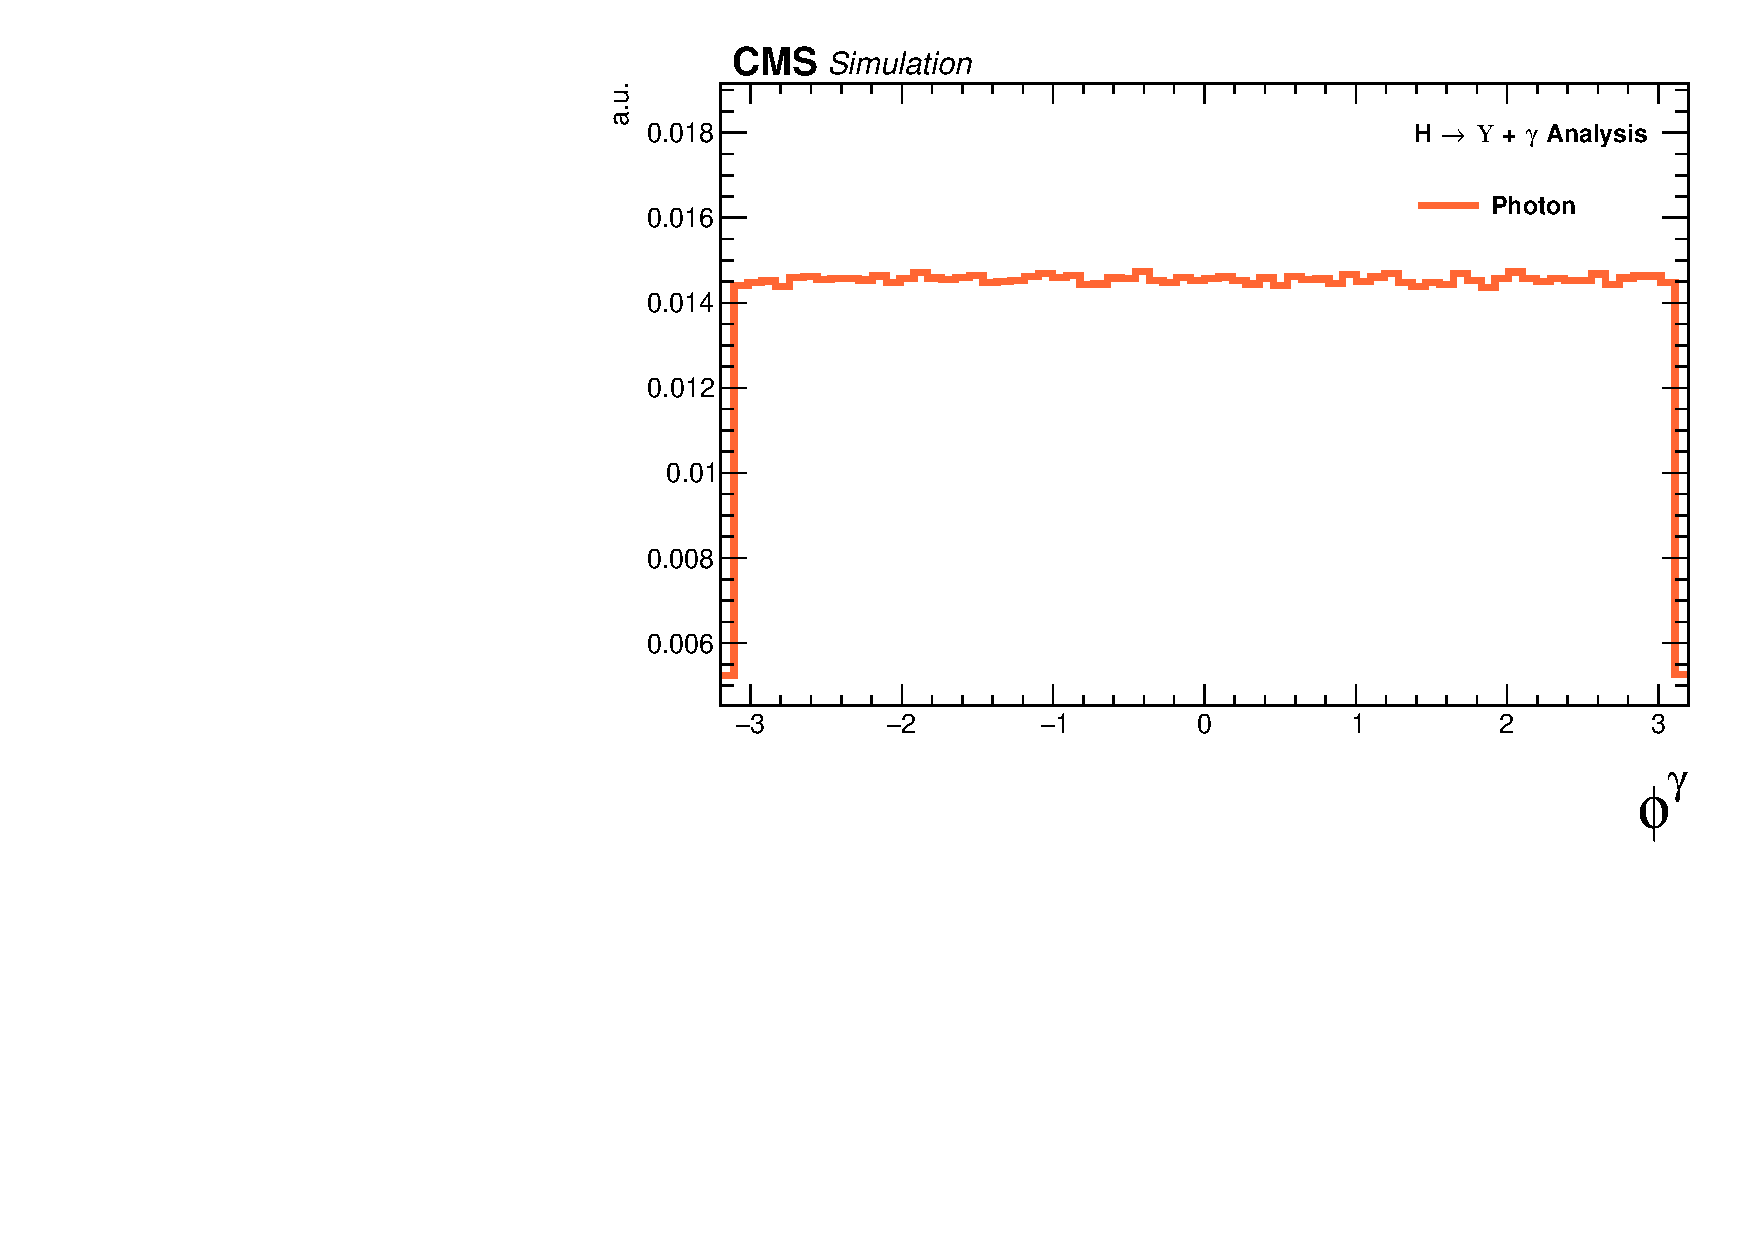
\includegraphics[width=0.45\textwidth]{figures_and_tables/outputPlots/HtoUpsilon_Cat0_ZZZZZ/mc/unpolarized/h_Gen_Photon_phi}
%\hspace*{1.cm}
%Delta R mu+ photon
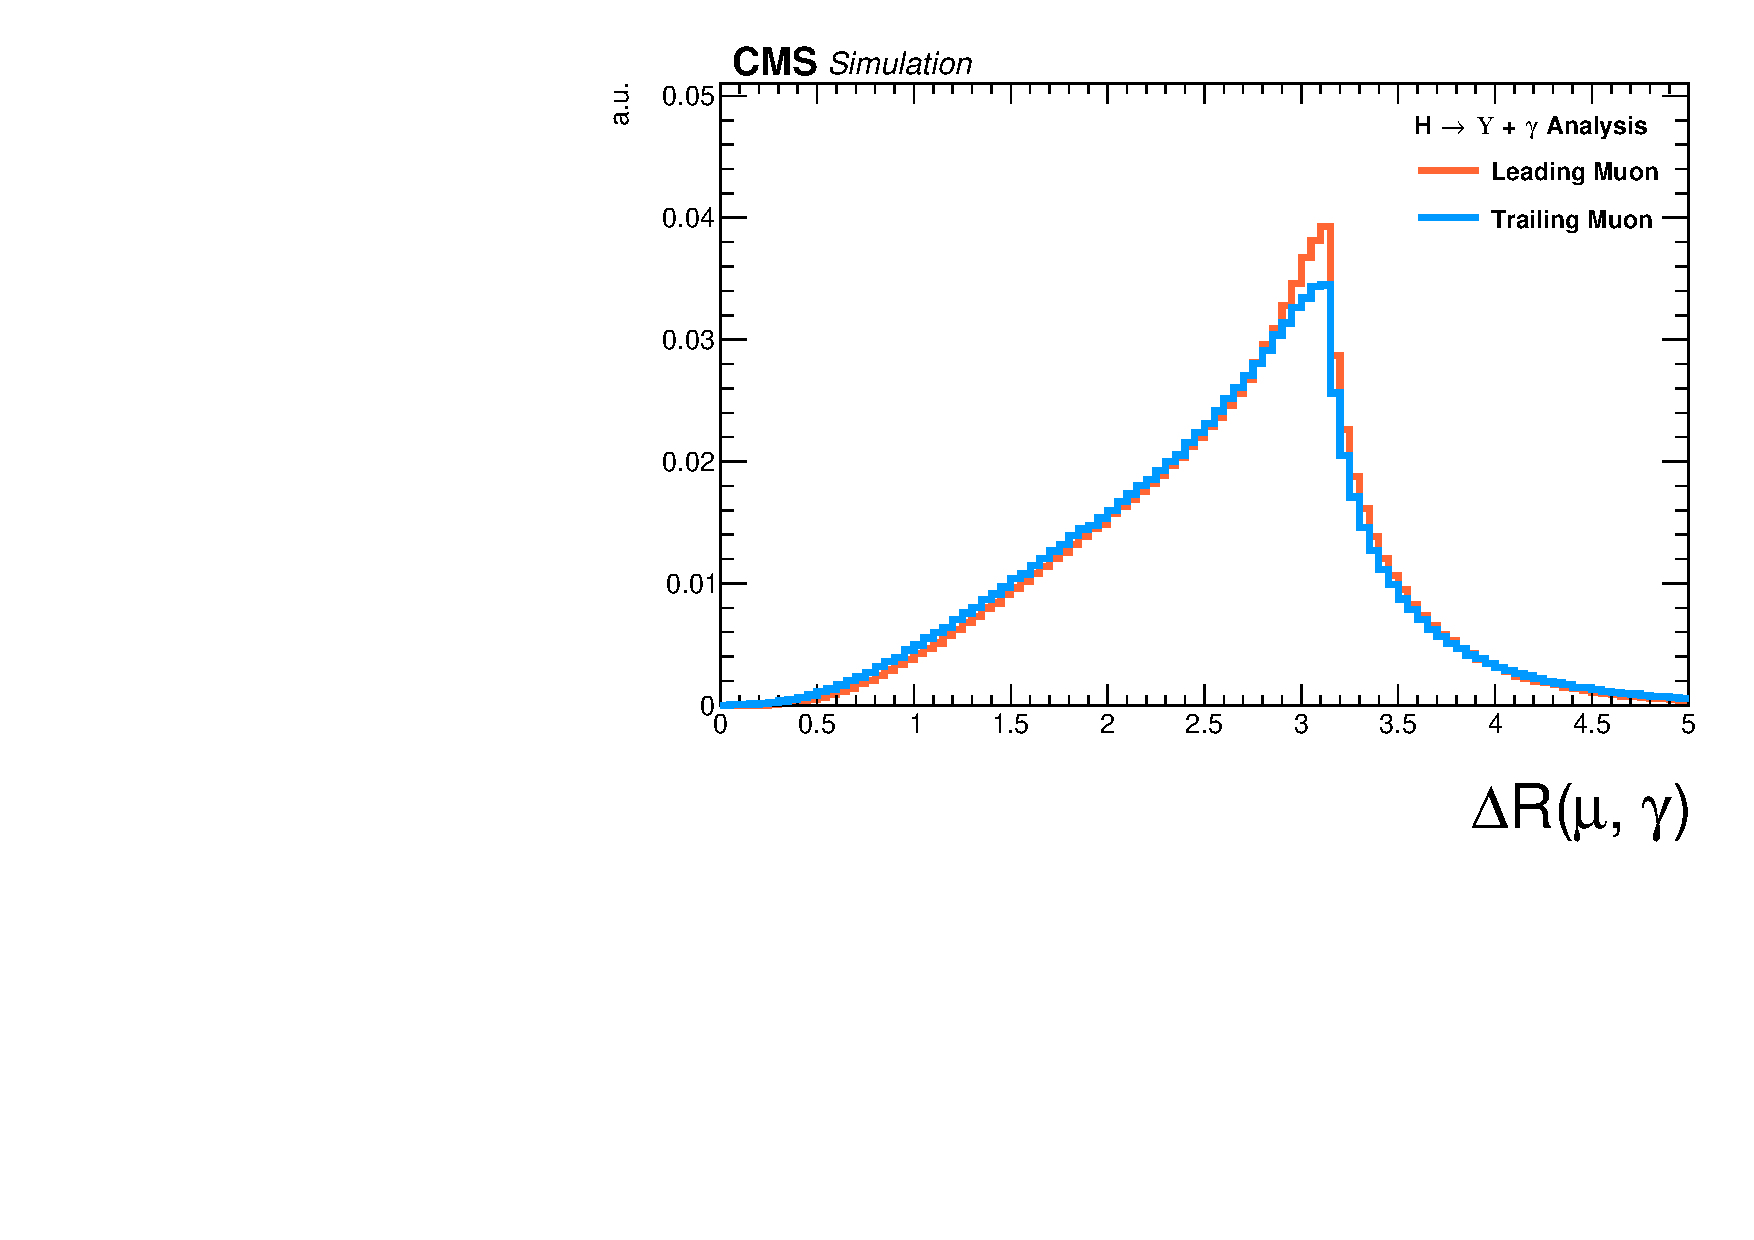
\includegraphics[width=0.45\textwidth]{figures_and_tables/outputPlots/HtoUpsilon_Cat0_ZZZZZ/mc/unpolarized/h_Gen_deltaR_Mu_Photon}
%\hspace*{1.cm}
%Upsilon
%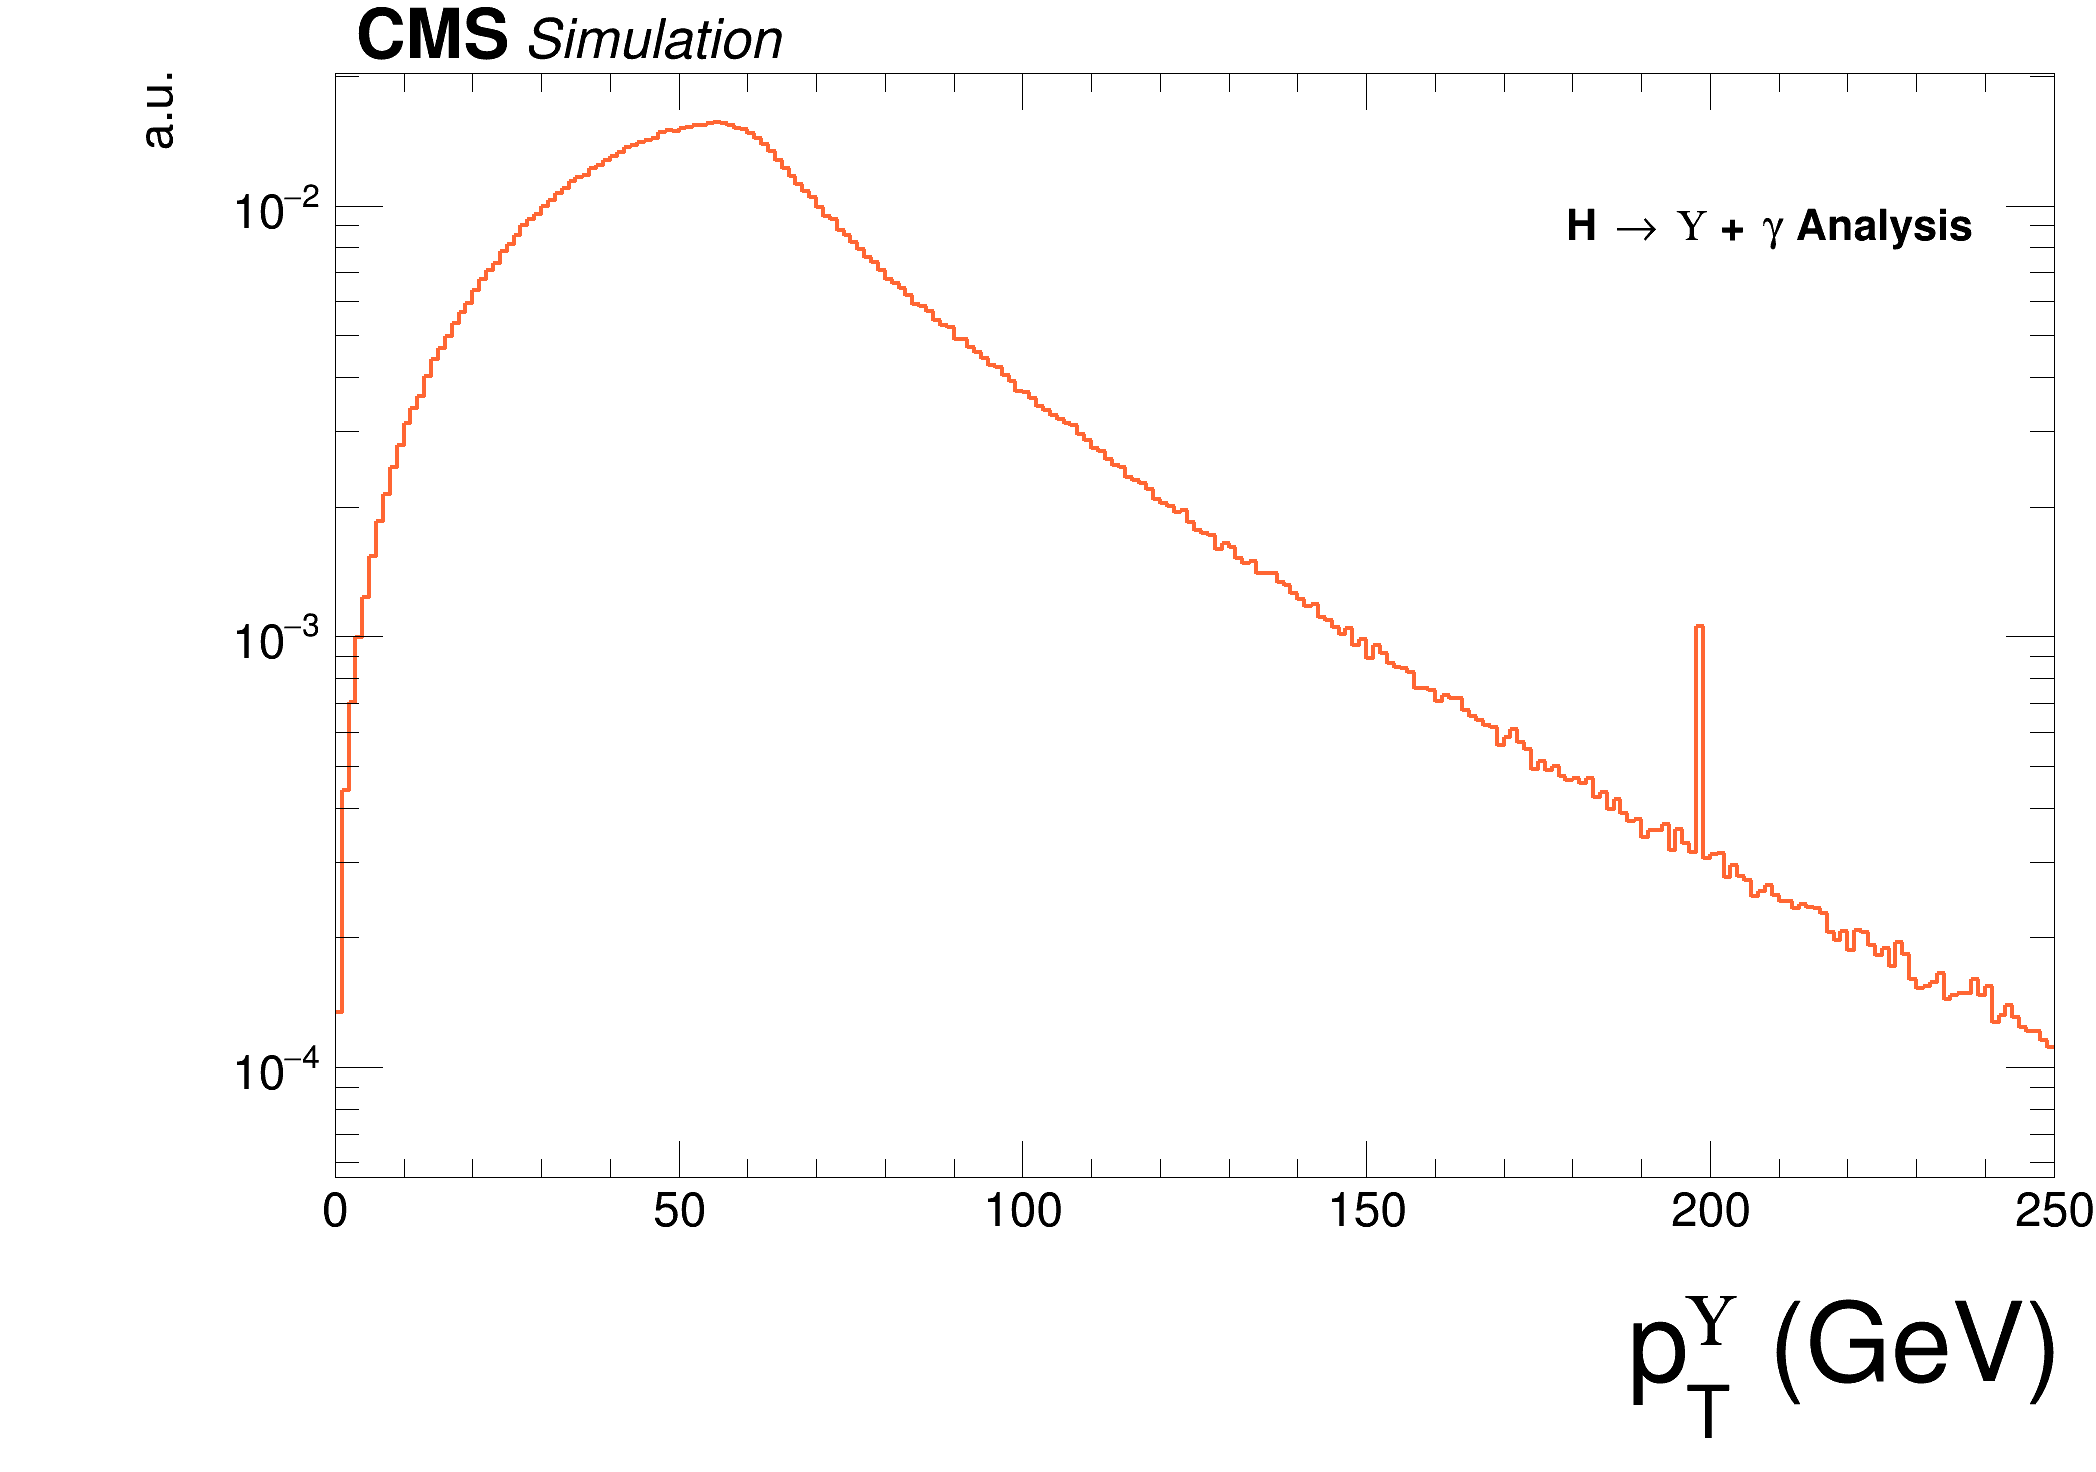
\includegraphics[width=0.25\textwidth]{figures_and_tables/outputPlots/HtoUpsilon_Cat0_ZZZZZ/mc/unpolarized/h_Gen_Upsilon_Pt}
%\hspace*{1.cm}
%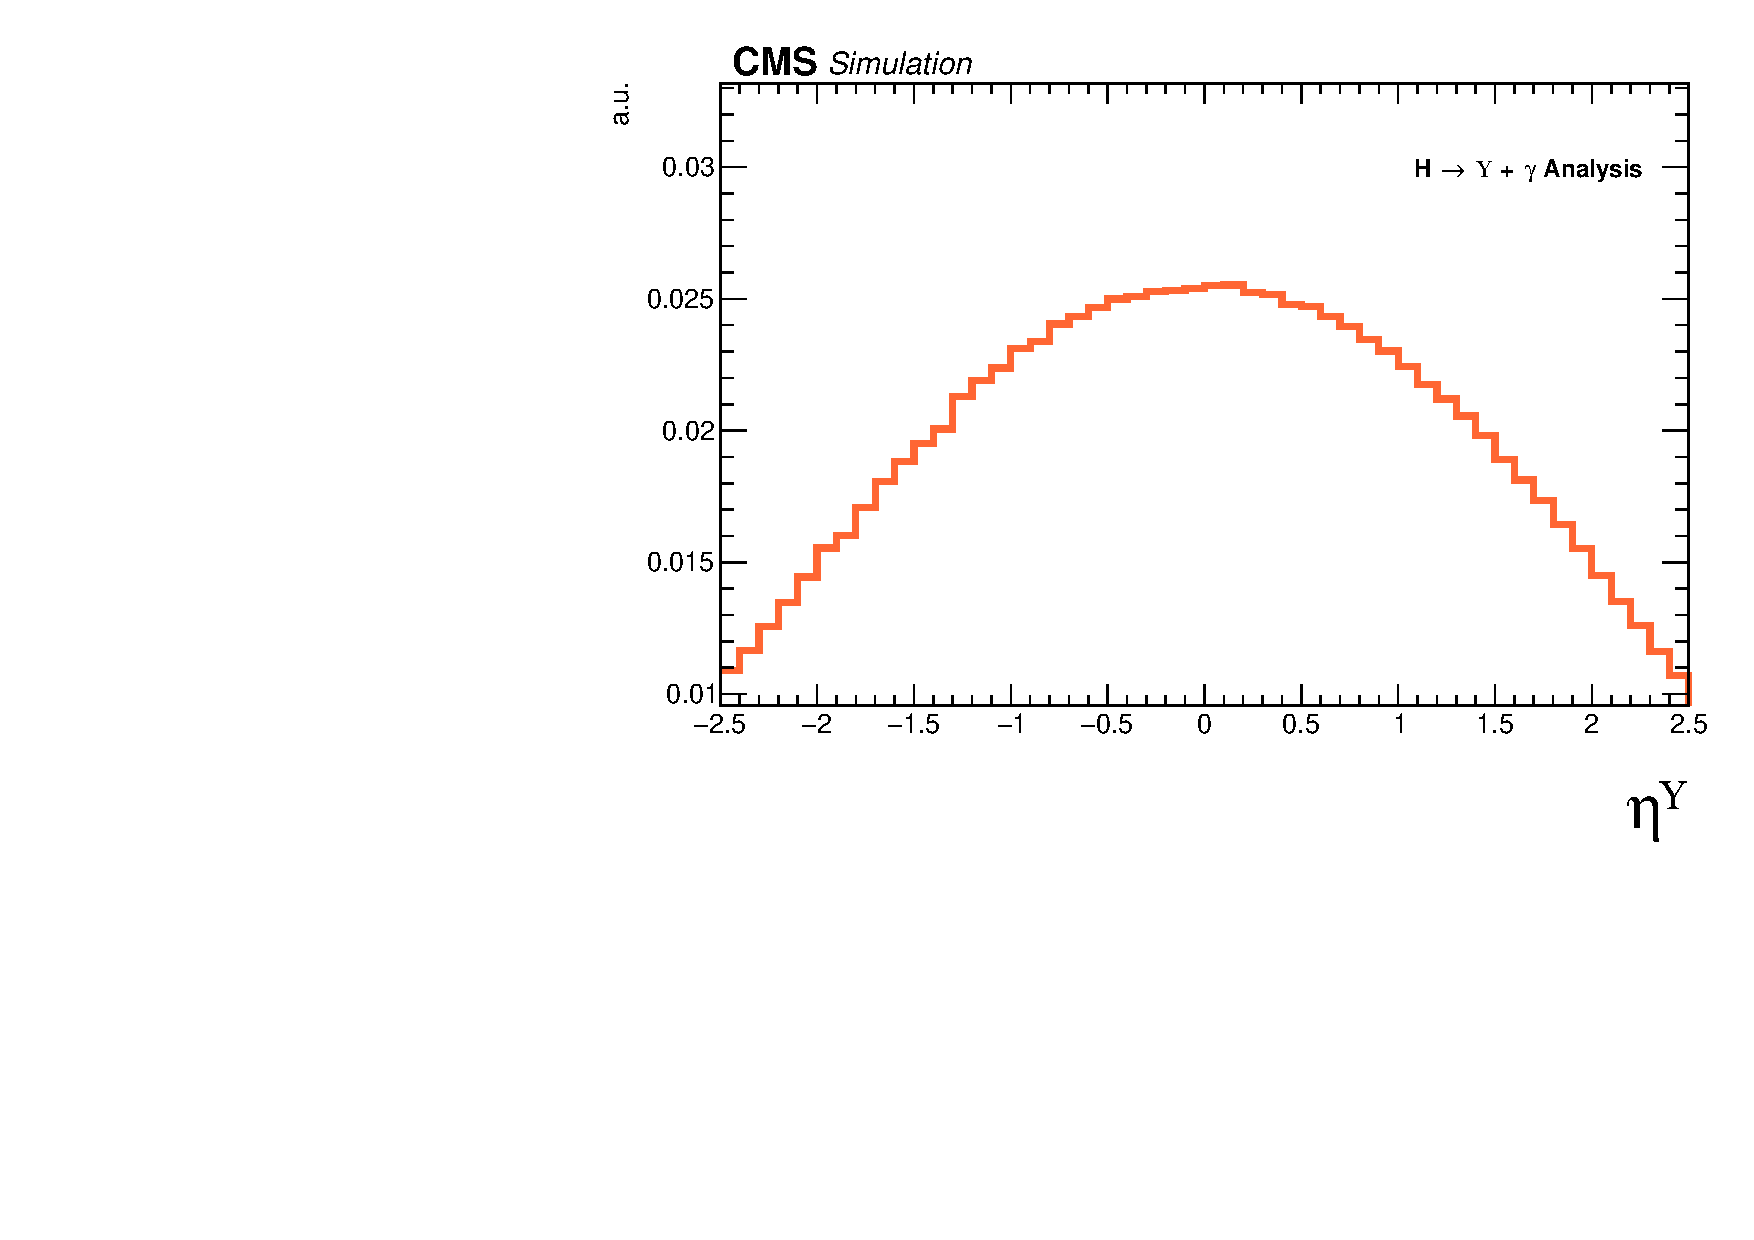
\includegraphics[width=0.25\textwidth]{figures_and_tables/outputPlots/HtoUpsilon_Cat0_ZZZZZ/mc/unpolarized/h_Gen_Upsilon_eta}
%\hspace*{1.cm}
%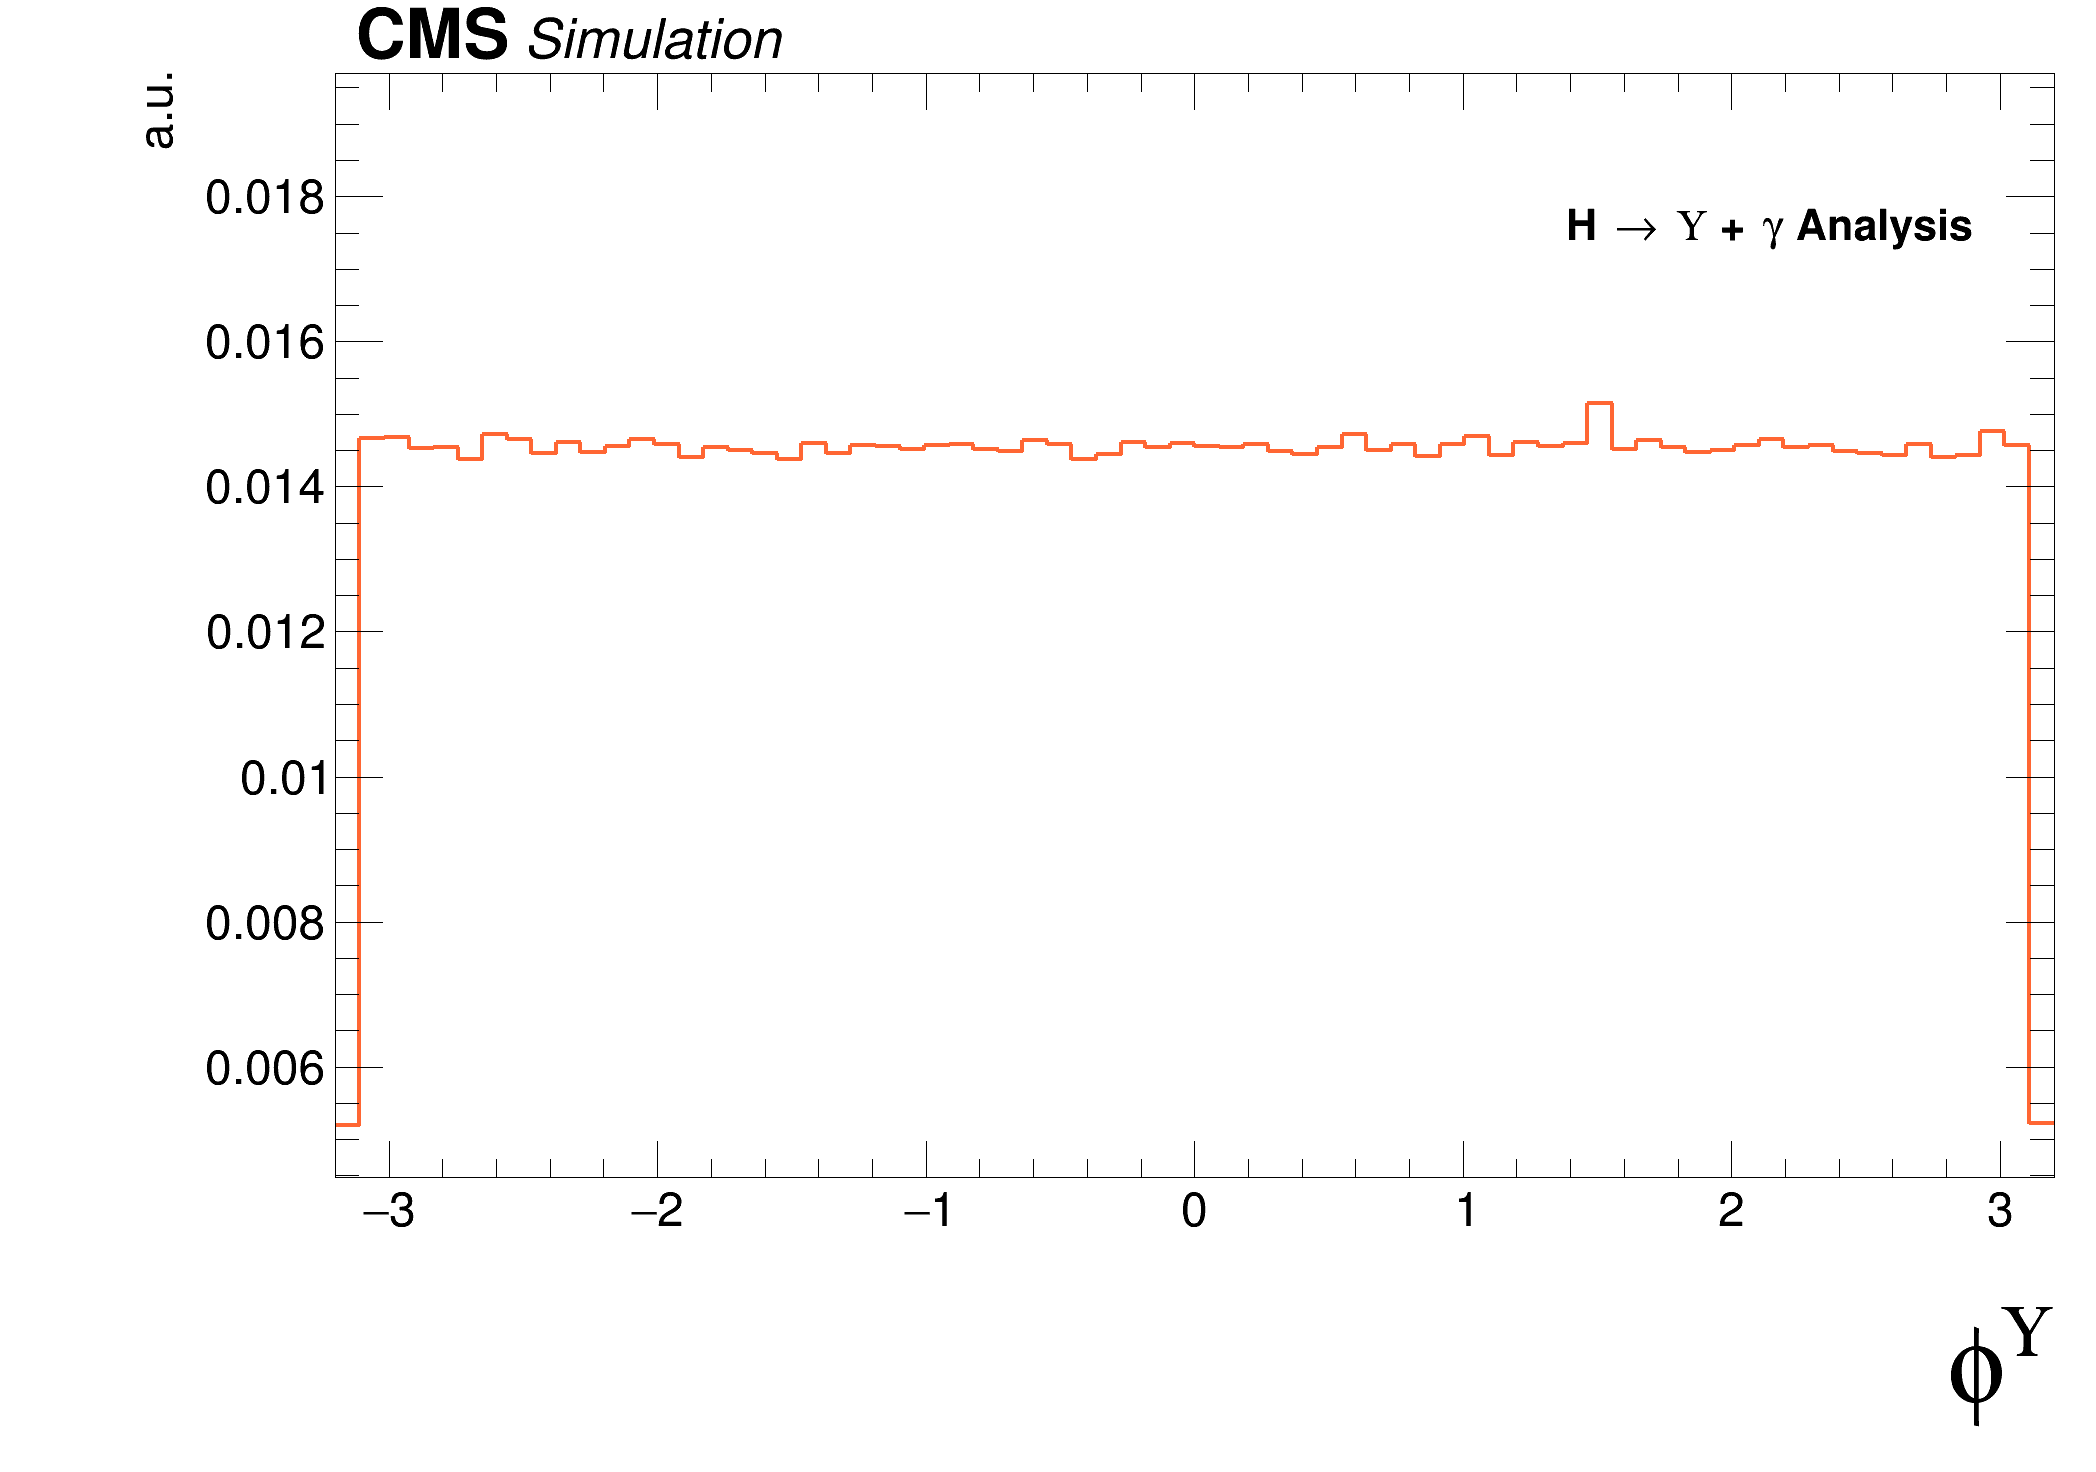
\includegraphics[width=0.25\textwidth]{figures_and_tables/outputPlots/HtoUpsilon_Cat0_ZZZZZ/mc/unpolarized/h_Gen_Upsilon_phi}
%\hspace*{1.cm}
%Z
%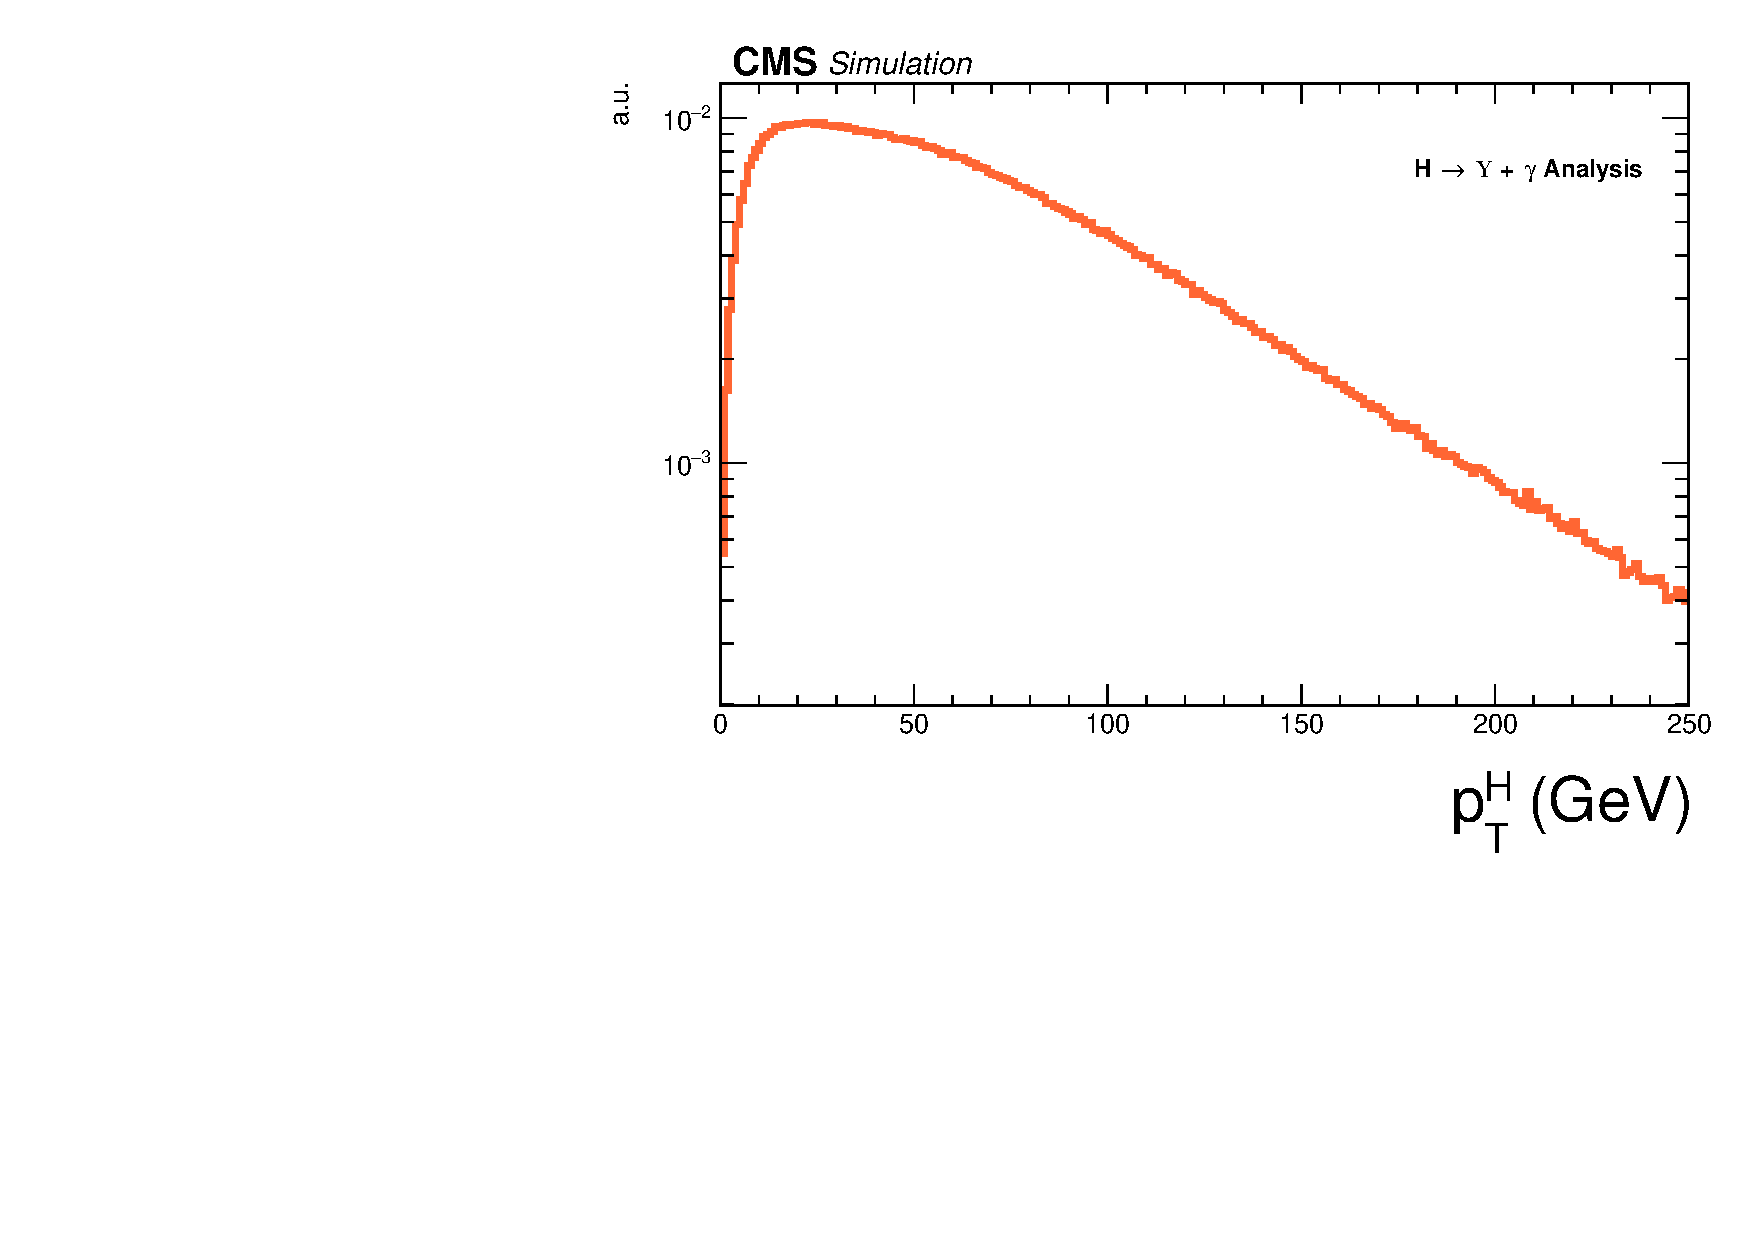
\includegraphics[width=0.25\textwidth]{figures_and_tables/outputPlots/HtoUpsilon_Cat0_ZZZZZ/mc/unpolarized/h_Gen_Z_Pt}
%\hspace*{1.cm}
%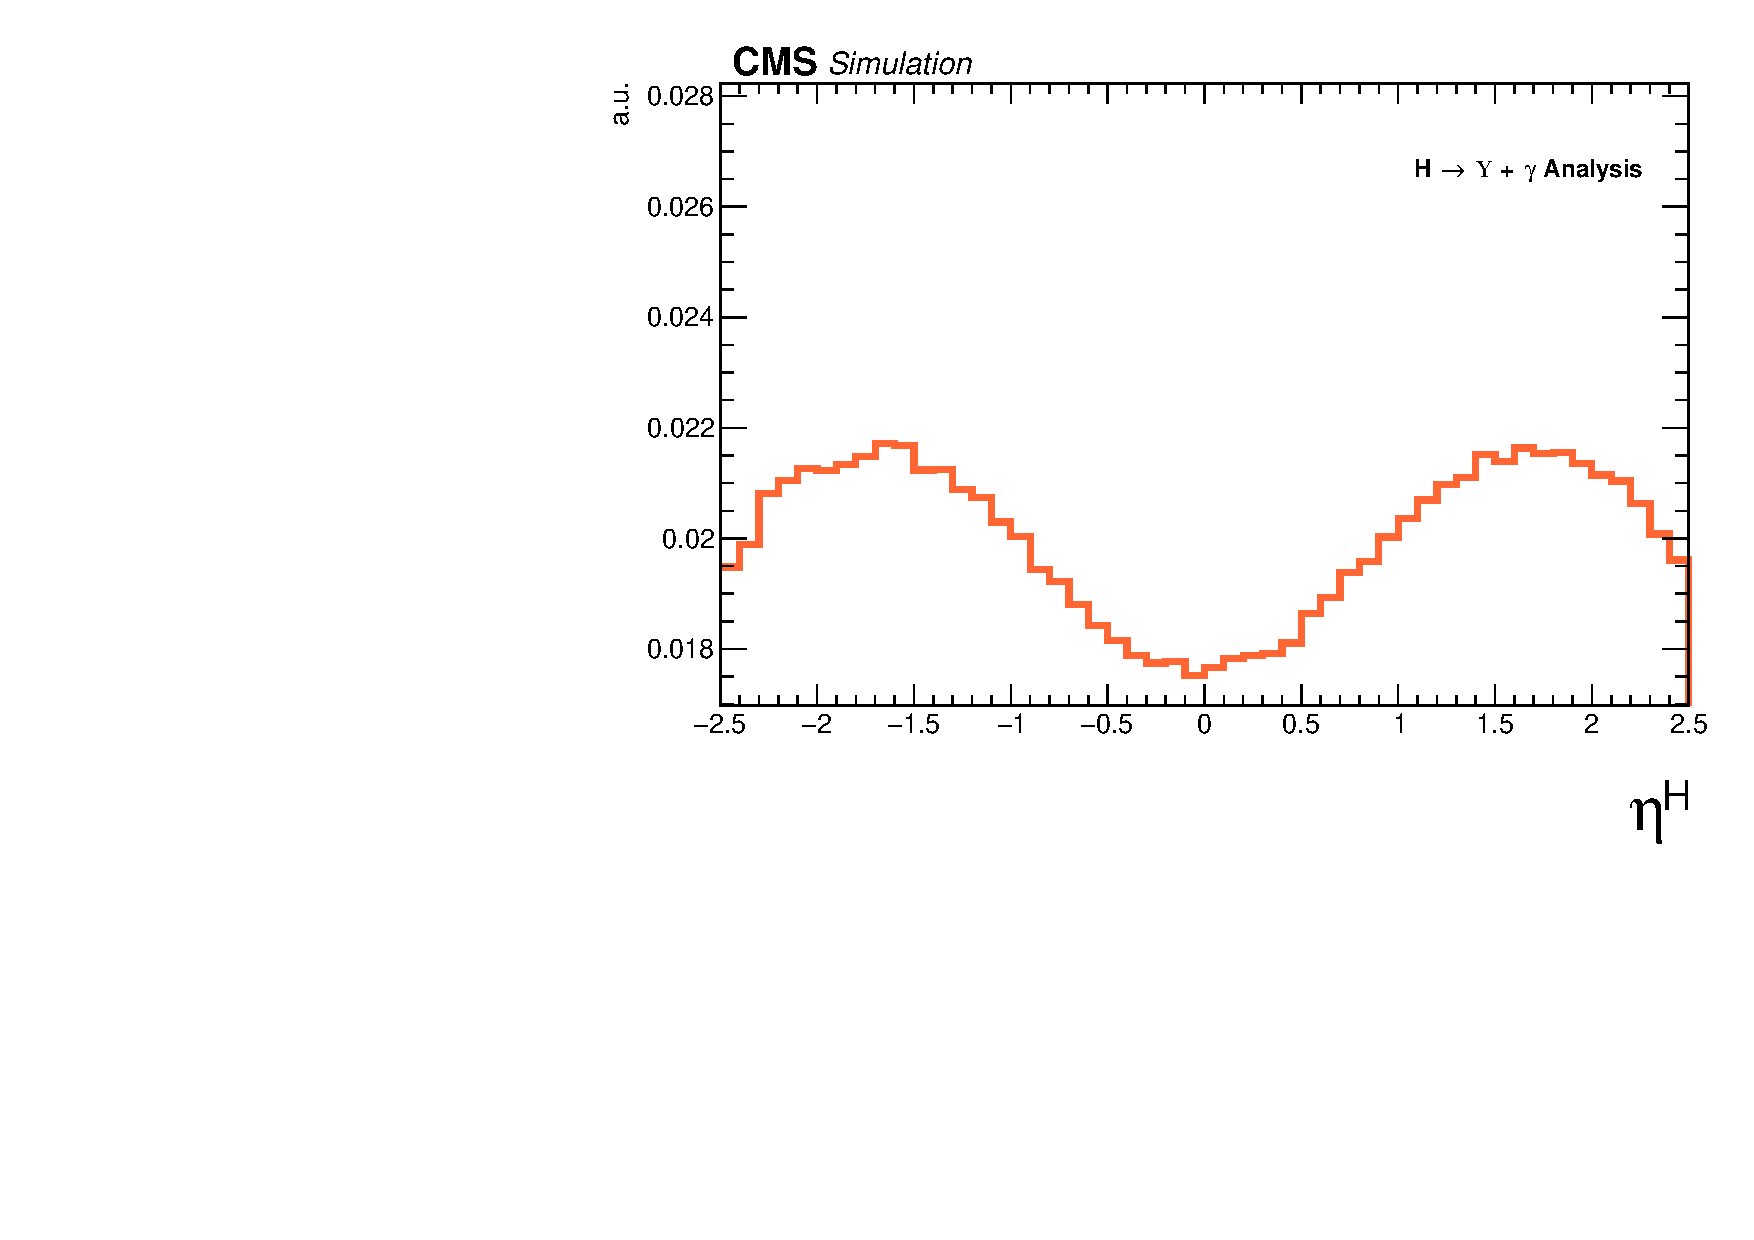
\includegraphics[width=0.25\textwidth]{figures_and_tables/outputPlots/HtoUpsilon_Cat0_ZZZZZ/mc/unpolarized/h_Gen_Z_eta}
%\hspace*{1.cm}
%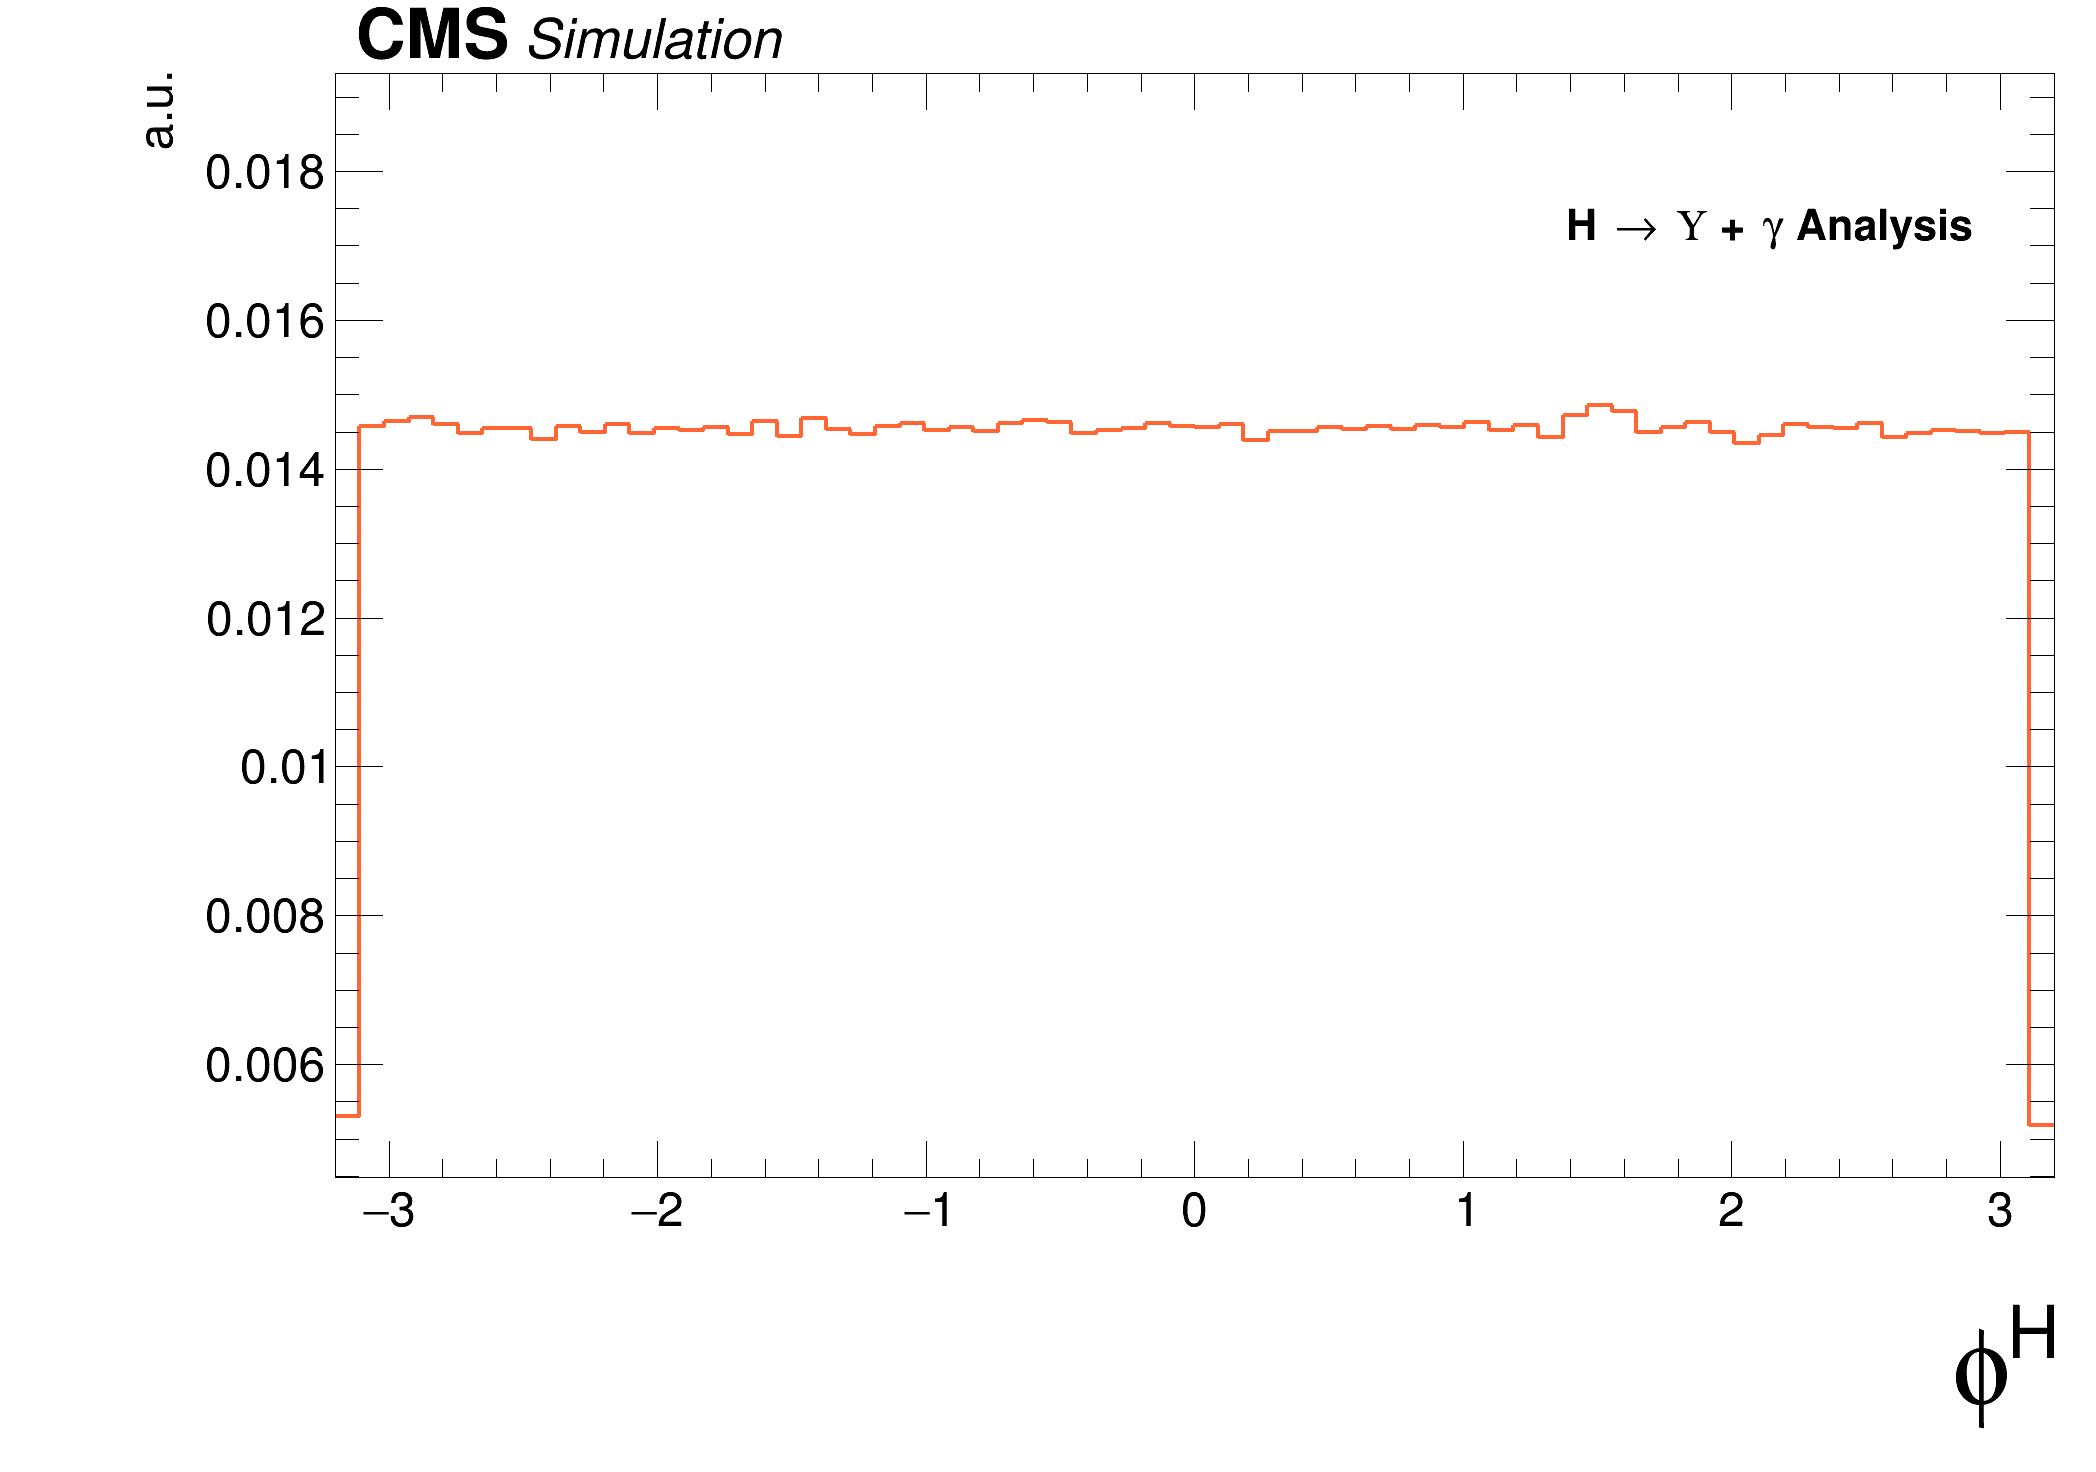
\includegraphics[width=0.25\textwidth]{figures_and_tables/outputPlots/HtoUpsilon_Cat0_ZZZZZ/mc/unpolarized/h_Gen_Z_phi}
%\hspace*{1.cm}
%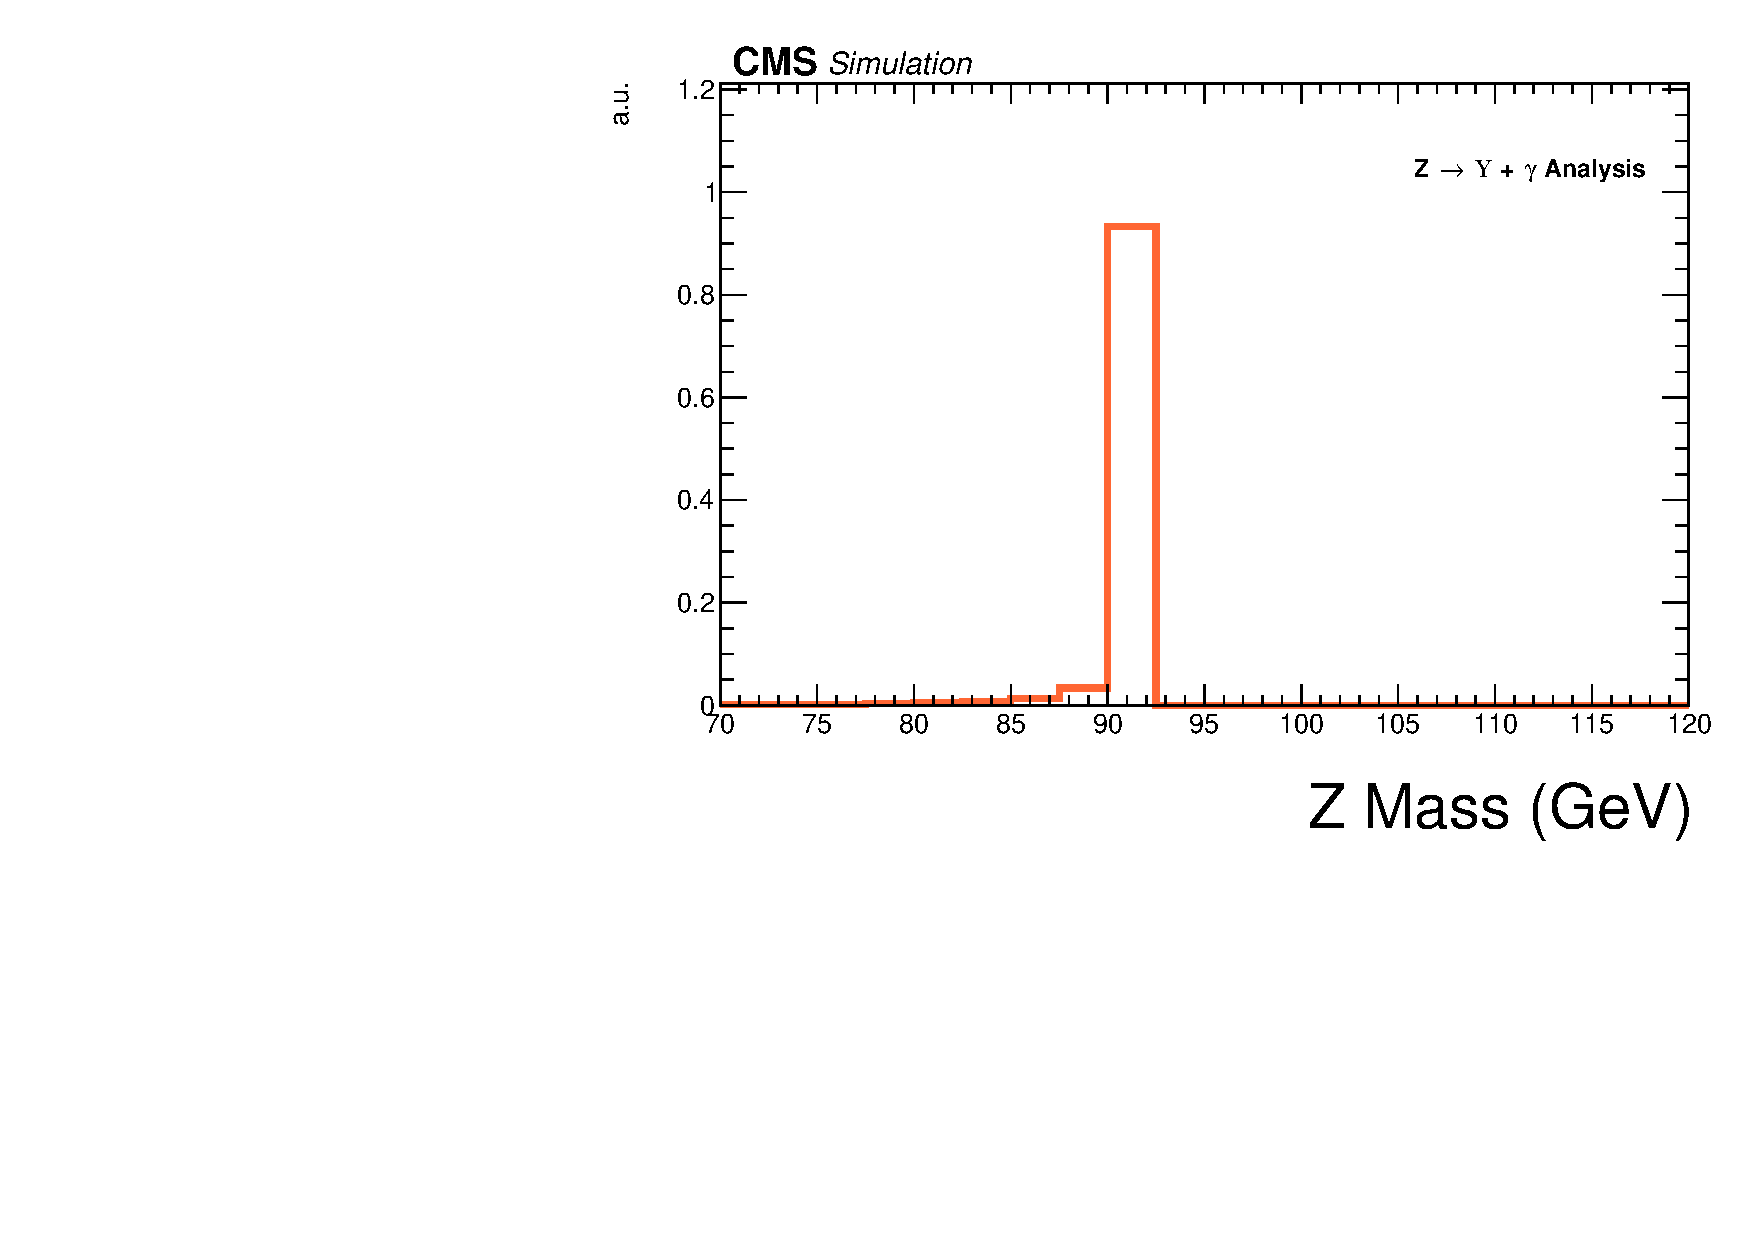
\includegraphics[width=0.25\textwidth]{figures_and_tables/outputPlots/ZtoUpsilon_Cat0_ZZZZZ/mc/unpolarized/h_Gen_Z_Mass}
%\hspace*{1.cm}
\end{center}%\vspace*{-.5cm}
\caption{Generator level distributions of main variables for $H\rightarrow  \Upsilon(1S,2S,3S) + \gamma$ : Transverse momenta of the leading/trailing $\PT$ muon and the photon, pseudorapidity ($\eta$) and $\phi$ of the muons and the photon, distances $\Delta R$ between the two muons and between the muons and the photon.All the distributions shown in the figure are normalized to the unity of area.}
\label{fig:MC_HtoUpsilon_Cat0}
\end{figure}

